% Generated fragments require trusted human review before compilation.
% This binder never requests shell escape or runs external tools.
\documentclass[11pt]{article}
% Trusted shared apparatus. Requires LuaLaTeX; never use shell escape.
\usepackage{fontspec}
\defaultfontfeatures{Ligatures=TeX}
\IfFontExistsTF{Noto Serif}{\setmainfont{Noto Serif}}{%
  \IfFontExistsTF{DejaVu Serif}{\setmainfont{DejaVu Serif}}{%
    \IfFontExistsTF{Times New Roman}{\setmainfont{Times New Roman}}{%
      \PackageError{gelfand-binder}{No configured Cyrillic serif font installed}{Install Noto Serif or DejaVu Serif, or select an installed Cyrillic font.}%
    }%
  }%
}
\IfFontExistsTF{Noto Sans}{\setsansfont{Noto Sans}}{%
  \IfFontExistsTF{DejaVu Sans}{\setsansfont{DejaVu Sans}}{\setsansfont{Arial}}%
}
\IfFontExistsTF{Noto Sans Mono}{\setmonofont{Noto Sans Mono}}{%
  \IfFontExistsTF{DejaVu Sans Mono}{\setmonofont{DejaVu Sans Mono}}{\setmonofont{Courier New}}%
}
\usepackage[a4paper,margin=22mm]{geometry}
\usepackage{amsmath,amssymb,amsthm,mathtools}
\usepackage{xcolor}
\usepackage{tikz}
\usepackage{tikz-cd}
\usetikzlibrary{arrows.meta,positioning,calc}
\usepackage{hyperref}
\hypersetup{unicode=true,colorlinks=true,linkcolor=blue,pdftitle={Gelfand transcription binder}}
\newtheorem{theorem}{Theorem}
\newtheorem{lemma}{Lemma}
\newtheorem{proposition}{Proposition}
\newtheorem{corollary}{Corollary}
\theoremstyle{definition}
\newtheorem{definition}{Definition}
\newtheorem{example}{Example}
\theoremstyle{remark}
\newtheorem{remark}{Remark}
\setlength{\parindent}{0pt}
\setlength{\parskip}{0.55em}
\setlength{\emergencystretch}{3em}
\newcommand{\SourcePage}[2]{%
  \clearpage\phantomsection\label{#1:source-page}%
  \addcontentsline{toc}{subsection}{#1}%
  {\small\sffamily\color{blue!60!black}Source scan frame: #1; visible page/leaf label: #2}\par\medskip%
}
\newcommand{\Unclear}[3]{%
  \begingroup\color{orange!70!black}%
  [Unresolved reading #1/#2: #3]\endgroup%
}
\newcommand{\Incomplete}[3]{%
  \par\begingroup\color{red!65!black}\textbf{Incomplete #1/#2:} #3\endgroup\par%
}
\newcommand{\SourceFigure}[3]{%
  \par\begingroup\color{blue!60!black}\textbf{\hyperref[#1:source-page]{Source figure #1/#2}:} #3%
  \par\textit{Consult the authoritative scan at this locator.}\endgroup\par%
}



% Reader layout only. Original diplomatic text is retained verbatim.
\setlength{\parskip}{0.35em}
\setlength{\emergencystretch}{4em}
\renewcommand{\SourcePage}[2]{%
  \par\addvspace{1em}\phantomsection\label{#1:source-page}%
  \addcontentsline{toc}{subsection}{#1}%
  {\footnotesize\sffamily\color{blue!55!black}#1%
    \def\givenlabel{#2}\def\nolabel{unlabelled}%
    \ifx\givenlabel\nolabel\else\quad[номер в источнике: #2]\fi
  }\par\nobreak\smallskip%
}
\renewcommand{\Unclear}[3]{%
  \begingroup\color{orange!65!black}%
  \ifmmode\text{[неясно: #3]}\else[неясно: #3]\fi\endgroup%
}
\renewcommand{\Incomplete}[3]{%
  \par\begingroup\color{red!60!black}\textbf{Неразобранный фрагмент:} #3%
  \endgroup\par%
}
\renewcommand{\SourceFigure}[3]{%
  \par\begingroup\color{blue!55!black}\textbf{Рисунок:} #3%
  \par{\small\textit{Исходный рисунок: \hyperref[#1:source-page]{#1}, #2.}}%
  \endgroup\par%
}
\hypersetup{pdftitle={Семинар И. М. Гельфанда. Дипломатическая транскрипция},pdfauthor={},pdfsubject={Русское рабочее издание с отмеченными сомнительными чтениями}}

\usepackage[normalem]{ulem}
\usepackage{newunicodechar}
\usepackage{adjustbox}
\newfontfamily\SourceSymbolFont{Segoe UI Symbol}
\newfontfamily\SourceCJKFont{MS Gothic}
\let\DiplomaticMathUnderline\underline
\renewcommand{\underline}[1]{\ifmmode\DiplomaticMathUnderline{#1}\else\uline{#1}\fi}
\newunicodechar{→}{\ifmmode\text{{\SourceSymbolFont\char"2192}}\else{\SourceSymbolFont\char"2192}\fi}
\newunicodechar{⇒}{\ifmmode\text{{\SourceSymbolFont\char"21D2}}\else{\SourceSymbolFont\char"21D2}\fi}
\newunicodechar{∀}{\ifmmode\text{{\SourceSymbolFont\char"2200}}\else{\SourceSymbolFont\char"2200}\fi}
\newunicodechar{∂}{\ifmmode\text{{\SourceSymbolFont\char"2202}}\else{\SourceSymbolFont\char"2202}\fi}
\newunicodechar{∈}{\ifmmode\text{{\SourceSymbolFont\char"2208}}\else{\SourceSymbolFont\char"2208}\fi}
\newunicodechar{∌}{\ifmmode\text{{\SourceSymbolFont\char"220C}}\else{\SourceSymbolFont\char"220C}\fi}
\newunicodechar{√}{\ifmmode\text{{\SourceSymbolFont\char"221A}}\else{\SourceSymbolFont\char"221A}\fi}
\newunicodechar{∞}{\ifmmode\text{{\SourceSymbolFont\char"221E}}\else{\SourceSymbolFont\char"221E}\fi}
\newunicodechar{∧}{\ifmmode\text{{\SourceSymbolFont\char"2227}}\else{\SourceSymbolFont\char"2227}\fi}
\newunicodechar{∩}{\ifmmode\text{{\SourceSymbolFont\char"2229}}\else{\SourceSymbolFont\char"2229}\fi}
\newunicodechar{∪}{\ifmmode\text{{\SourceSymbolFont\char"222A}}\else{\SourceSymbolFont\char"222A}\fi}
\newunicodechar{∫}{\ifmmode\text{{\SourceSymbolFont\char"222B}}\else{\SourceSymbolFont\char"222B}\fi}
\newunicodechar{∴}{\ifmmode\text{{\SourceSymbolFont\char"2234}}\else{\SourceSymbolFont\char"2234}\fi}
\newunicodechar{∼}{\ifmmode\text{{\SourceSymbolFont\char"223C}}\else{\SourceSymbolFont\char"223C}\fi}
\newunicodechar{≈}{\ifmmode\text{{\SourceSymbolFont\char"2248}}\else{\SourceSymbolFont\char"2248}\fi}
\newunicodechar{≠}{\ifmmode\text{{\SourceSymbolFont\char"2260}}\else{\SourceSymbolFont\char"2260}\fi}
\newunicodechar{≤}{\ifmmode\text{{\SourceSymbolFont\char"2264}}\else{\SourceSymbolFont\char"2264}\fi}
\newunicodechar{≥}{\ifmmode\text{{\SourceSymbolFont\char"2265}}\else{\SourceSymbolFont\char"2265}\fi}
\newunicodechar{⊕}{\ifmmode\text{{\SourceSymbolFont\char"2295}}\else{\SourceSymbolFont\char"2295}\fi}
\newunicodechar{⊗}{\ifmmode\text{{\SourceSymbolFont\char"2297}}\else{\SourceSymbolFont\char"2297}\fi}
\newunicodechar{①}{\ifmmode\text{{\SourceSymbolFont\char"2460}}\else{\SourceSymbolFont\char"2460}\fi}
\newunicodechar{②}{\ifmmode\text{{\SourceSymbolFont\char"2461}}\else{\SourceSymbolFont\char"2461}\fi}
\newunicodechar{③}{\ifmmode\text{{\SourceSymbolFont\char"2462}}\else{\SourceSymbolFont\char"2462}\fi}
\newunicodechar{④}{\ifmmode\text{{\SourceSymbolFont\char"2463}}\else{\SourceSymbolFont\char"2463}\fi}
\newunicodechar{Ⓗ}{\ifmmode\text{{\SourceSymbolFont\char"24BD}}\else{\SourceSymbolFont\char"24BD}\fi}
\newunicodechar{〃}{\ifmmode\text{{\SourceCJKFont\char"3003}}\else{\SourceCJKFont\char"3003}\fi}


% Reader revision 3. Annotation wording and candidates remain unchanged.
\setmainfont{NotoSerif-Regular.ttf}[Path=C:/Windows/Fonts/,ItalicFont=NotoSerif-Italic.ttf,BoldFont=NotoSerif-Bold.ttf,BoldItalicFont=NotoSerif-BoldItalic.ttf]
\usetikzlibrary{shapes.geometric,decorations.pathreplacing,decorations.markings,patterns,fit}
\newsavebox{\ReaderAnnotationBox}
\newcommand{\ReaderAnnotation}[1]{%
  \sbox{\ReaderAnnotationBox}{[неясно: #1]}%
  \ifdim\wd\ReaderAnnotationBox>.70\linewidth
    \parbox[t]{.70\linewidth}{\raggedright[неясно: #1]}%
  \else\usebox{\ReaderAnnotationBox}\fi%
}
\ExplSyntaxOn
\cs_new_protected:Npn \reader_unclear_candidate:n #1
 {
  \tl_set:Nx \l_tmpa_tl { \tl_to_str:n {#1} }
  % Text explicitly guarded inside a mathematical candidate remains math-safe.
  \regex_replace_all:nnN { \\(?:text|textrm|textnormal|textbf|operatorname)\s*\{[^{}]*\} } { } \l_tmpa_tl
  \regex_match:nVTF { [\x{0400}-\x{052F}] | \$ } \l_tmpa_tl
   { \ifmmode \text{\ReaderAnnotation{#1}} \else \ReaderAnnotation{#1} \fi }
   {
    \ifmmode
      \mathord{\underset{\text{\tiny неясно}}{#1}}
    \else
      \regex_match:nVTF { [_^] | \\ } \l_tmpa_tl
       { \ensuremath{[\text{неясно:~}#1]} }
       { \ReaderAnnotation{#1} }
    \fi
   }
 }
\RenewDocumentCommand \Unclear { m m m }
 { \begingroup\color{orange!65!black}\reader_unclear_candidate:n{#3}\endgroup }
\ExplSyntaxOff
\newsavebox{\ReaderIncompleteBox}
\newcommand{\ReaderApparatusRef}[2]{%
 \begingroup\ifnum#2=1\color{orange!65!black}\else\color{red!60!black}\fi%
 \ifmmode\text{\scriptsize[прим.\,#1]}\else{\scriptsize[прим.\,#1]}\fi\endgroup%
}
\newcommand{\ReaderNotesStart}[1]{%
 \par\addvspace{.4em}\begingroup\small%
 \textbf{Примечания к кадру #1.}\par%
}
\newcommand{\ReaderNote}[2]{\par\noindent[#1]\quad#2\par}
\newcommand{\ReaderNotesEnd}{\endgroup\par\addvspace{.4em}}
\newcommand{\ReaderIncompleteNote}[1]{%
 \sbox{\ReaderIncompleteBox}{\textbf{Неразобранный фрагмент:} #1}%
 \ifdim\wd\ReaderIncompleteBox>.70\linewidth
  \parbox[t]{.70\linewidth}{\raggedright\textbf{Неразобранный фрагмент:} #1}%
 \else\usebox{\ReaderIncompleteBox}\fi%
}
\renewcommand{\Incomplete}[3]{%
 \ifmmode\text{\color{red!60!black}\ReaderIncompleteNote{#3}}%
 \else\leavevmode\begingroup\color{red!60!black}\ReaderIncompleteNote{#3}\endgroup\fi%
}
% Ragged right avoids stretching long untranslated abbreviations into margins.
\AtBeginDocument{\raggedright}
\newunicodechar{А}{\ifmmode\text{\char"410\relax}\else\char"410\relax\fi}
\newunicodechar{Б}{\ifmmode\text{\char"411\relax}\else\char"411\relax\fi}
\newunicodechar{В}{\ifmmode\text{\char"412\relax}\else\char"412\relax\fi}
\newunicodechar{Г}{\ifmmode\text{\char"413\relax}\else\char"413\relax\fi}
\newunicodechar{Д}{\ifmmode\text{\char"414\relax}\else\char"414\relax\fi}
\newunicodechar{Е}{\ifmmode\text{\char"415\relax}\else\char"415\relax\fi}
\newunicodechar{Ж}{\ifmmode\text{\char"416\relax}\else\char"416\relax\fi}
\newunicodechar{З}{\ifmmode\text{\char"417\relax}\else\char"417\relax\fi}
\newunicodechar{И}{\ifmmode\text{\char"418\relax}\else\char"418\relax\fi}
\newunicodechar{Й}{\ifmmode\text{\char"419\relax}\else\char"419\relax\fi}
\newunicodechar{К}{\ifmmode\text{\char"41A\relax}\else\char"41A\relax\fi}
\newunicodechar{Л}{\ifmmode\text{\char"41B\relax}\else\char"41B\relax\fi}
\newunicodechar{М}{\ifmmode\text{\char"41C\relax}\else\char"41C\relax\fi}
\newunicodechar{Н}{\ifmmode\text{\char"41D\relax}\else\char"41D\relax\fi}
\newunicodechar{О}{\ifmmode\text{\char"41E\relax}\else\char"41E\relax\fi}
\newunicodechar{П}{\ifmmode\text{\char"41F\relax}\else\char"41F\relax\fi}
\newunicodechar{Р}{\ifmmode\text{\char"420\relax}\else\char"420\relax\fi}
\newunicodechar{С}{\ifmmode\text{\char"421\relax}\else\char"421\relax\fi}
\newunicodechar{Т}{\ifmmode\text{\char"422\relax}\else\char"422\relax\fi}
\newunicodechar{У}{\ifmmode\text{\char"423\relax}\else\char"423\relax\fi}
\newunicodechar{Ф}{\ifmmode\text{\char"424\relax}\else\char"424\relax\fi}
\newunicodechar{Х}{\ifmmode\text{\char"425\relax}\else\char"425\relax\fi}
\newunicodechar{Ц}{\ifmmode\text{\char"426\relax}\else\char"426\relax\fi}
\newunicodechar{Ч}{\ifmmode\text{\char"427\relax}\else\char"427\relax\fi}
\newunicodechar{Ш}{\ifmmode\text{\char"428\relax}\else\char"428\relax\fi}
\newunicodechar{Щ}{\ifmmode\text{\char"429\relax}\else\char"429\relax\fi}
\newunicodechar{Ъ}{\ifmmode\text{\char"42A\relax}\else\char"42A\relax\fi}
\newunicodechar{Ы}{\ifmmode\text{\char"42B\relax}\else\char"42B\relax\fi}
\newunicodechar{Ь}{\ifmmode\text{\char"42C\relax}\else\char"42C\relax\fi}
\newunicodechar{Э}{\ifmmode\text{\char"42D\relax}\else\char"42D\relax\fi}
\newunicodechar{Ю}{\ifmmode\text{\char"42E\relax}\else\char"42E\relax\fi}
\newunicodechar{Я}{\ifmmode\text{\char"42F\relax}\else\char"42F\relax\fi}
\newunicodechar{а}{\ifmmode\text{\char"430\relax}\else\char"430\relax\fi}
\newunicodechar{б}{\ifmmode\text{\char"431\relax}\else\char"431\relax\fi}
\newunicodechar{в}{\ifmmode\text{\char"432\relax}\else\char"432\relax\fi}
\newunicodechar{г}{\ifmmode\text{\char"433\relax}\else\char"433\relax\fi}
\newunicodechar{д}{\ifmmode\text{\char"434\relax}\else\char"434\relax\fi}
\newunicodechar{е}{\ifmmode\text{\char"435\relax}\else\char"435\relax\fi}
\newunicodechar{ж}{\ifmmode\text{\char"436\relax}\else\char"436\relax\fi}
\newunicodechar{з}{\ifmmode\text{\char"437\relax}\else\char"437\relax\fi}
\newunicodechar{и}{\ifmmode\text{\char"438\relax}\else\char"438\relax\fi}
\newunicodechar{й}{\ifmmode\text{\char"439\relax}\else\char"439\relax\fi}
\newunicodechar{к}{\ifmmode\text{\char"43A\relax}\else\char"43A\relax\fi}
\newunicodechar{л}{\ifmmode\text{\char"43B\relax}\else\char"43B\relax\fi}
\newunicodechar{м}{\ifmmode\text{\char"43C\relax}\else\char"43C\relax\fi}
\newunicodechar{н}{\ifmmode\text{\char"43D\relax}\else\char"43D\relax\fi}
\newunicodechar{о}{\ifmmode\text{\char"43E\relax}\else\char"43E\relax\fi}
\newunicodechar{п}{\ifmmode\text{\char"43F\relax}\else\char"43F\relax\fi}
\newunicodechar{р}{\ifmmode\text{\char"440\relax}\else\char"440\relax\fi}
\newunicodechar{с}{\ifmmode\text{\char"441\relax}\else\char"441\relax\fi}
\newunicodechar{т}{\ifmmode\text{\char"442\relax}\else\char"442\relax\fi}
\newunicodechar{у}{\ifmmode\text{\char"443\relax}\else\char"443\relax\fi}
\newunicodechar{ф}{\ifmmode\text{\char"444\relax}\else\char"444\relax\fi}
\newunicodechar{х}{\ifmmode\text{\char"445\relax}\else\char"445\relax\fi}
\newunicodechar{ц}{\ifmmode\text{\char"446\relax}\else\char"446\relax\fi}
\newunicodechar{ч}{\ifmmode\text{\char"447\relax}\else\char"447\relax\fi}
\newunicodechar{ш}{\ifmmode\text{\char"448\relax}\else\char"448\relax\fi}
\newunicodechar{щ}{\ifmmode\text{\char"449\relax}\else\char"449\relax\fi}
\newunicodechar{ъ}{\ifmmode\text{\char"44A\relax}\else\char"44A\relax\fi}
\newunicodechar{ы}{\ifmmode\text{\char"44B\relax}\else\char"44B\relax\fi}
\newunicodechar{ь}{\ifmmode\text{\char"44C\relax}\else\char"44C\relax\fi}
\newunicodechar{э}{\ifmmode\text{\char"44D\relax}\else\char"44D\relax\fi}
\newunicodechar{ю}{\ifmmode\text{\char"44E\relax}\else\char"44E\relax\fi}
\newunicodechar{я}{\ifmmode\text{\char"44F\relax}\else\char"44F\relax\fi}
\newunicodechar{Ё}{\ifmmode\text{\char"401\relax}\else\char"401\relax\fi}
\newunicodechar{ё}{\ifmmode\text{\char"451\relax}\else\char"451\relax\fi}

\newunicodechar{æ}{\ifmmode\text{\char"E6\relax}\else\char"E6\relax\fi}
\newunicodechar{−}{\ifmmode\mathbin{\text{\SourceSymbolFont\char"2212\relax}}\else{\SourceSymbolFont\char"2212\relax}\fi}


% Reader-only pairing support; accepted raw bodies remain unchanged.
\RequirePackage{graphicx}
\RequirePackage{adjustbox}
\newcommand{\ReaderOriginalPanel}[2]{%
  \begin{minipage}[t]{.48\linewidth}\vspace{0pt}\centering
    \includegraphics[width=\linewidth,keepaspectratio]{#1}\par\smallskip
    {\scriptsize Оригинал рукописного рисунка: #2}\par
  \end{minipage}%
}
\newcommand{\ReaderDiagramPair}[3]{%
  \par\noindent\begingroup
  \ReaderOriginalPanel{#1}{#2}\hfill
  \begin{minipage}[t]{.48\linewidth}\vspace{0pt}\centering
    {\scriptsize Типографское воссоздание}\par\smallskip
    \begin{adjustbox}{max width=\linewidth}#3\end{adjustbox}\par
  \end{minipage}%
  \endgroup\par\smallskip
}
\newcommand{\ReaderDescriptionPair}[3]{%
  \par\noindent\begingroup
  \ReaderOriginalPanel{#1}{#2}\hfill
  \begin{minipage}[t]{.48\linewidth}\vspace{0pt}\raggedright
    {\scriptsize Типографское описание}\par\smallskip
    #3\par
  \end{minipage}%
  \endgroup\par\smallskip
}


\begin{document}
\begin{center}
{\Large Семинар И. М. Гельфанда}\par\medskip
{\LARGE Дипломатическая транскрипция}\par\bigskip
{\large Рабочее русское издание}\par\medskip
{\large Том 24 из 34. Архивная глава 024}\par\bigskip
Кадры GELFAND-P001133 -- GELFAND-P001185\par
\end{center}
\medskip
Сокращения, отменённые записи и сомнительные чтения сохранены.
Неразобранные фрагменты отмечены в тексте. Математические утверждения
источника переданы без молчаливых исправлений.

В текущем комплекте приняты 165 из 165 возвратов; учтены 1527 из 1527 кадров. Кадров без принятого возврата: 0.
Статусы кадров в отчётах о полноте: транскрибированы 1168, неразборчивы 357, частично прочитаны 1, недоступны 1.
Нерешённых записей журнала чтений: 6820.
Статус «неразборчивый» может отмечать локальную утрату зачёркнутой записи;
он не означает отсутствия всего кадра.
Сверка с рукописью продолжается. Рабочие журналы чтений и происхождения
данных сохранены отдельно.

Ограничения исходного комплекта: повреждённый исходный скан GELFAND-P000722; каталожные записи 603, 694 без сканов; в архивной главе 029 не перечислена часть 25.

Границы кадров показаны небольшими синими указателями; печатный текст
продолжается без обязательного разрыва страницы после каждого кадра.
\bigskip\hrule\bigskip
\SourcePage{GELFAND-P001133}{unlabelled}
\underline{31/X-83.}\qquad \underline{Сем. Гельфанда.}

\underline{Зелевинский.}

$\Lambda_n^k$ — однор. симм. многочлены от $x_1,\ldots,x_n$ степени $k$ (над $\mathbb Z$).

При $n\geq k$ $\Lambda_n^k$ не зависит от $n$.

Рассмотрим $\Lambda^k=\underset{\leftarrow\,n}{\lim}\Lambda_n^k$ и кольцо
$\Lambda=\bigoplus_{k\geq0}\Lambda^k$ всех симм. ф-й.

Элем. теория симм. ф-й: выд. 5 базисов и уст. связи между ними.

Разбиение:
\begin{equation*}
 \lambda=(\lambda_1\geq\lambda_2\geq\ldots)
 \qquad \text{(начиная с нек. места — нули)}
\end{equation*}
(все $\lambda_j$ — неотриц. целые).

$\lambda=(4,2,1)$ пример.\qquad $\lambda_i$ — части разбиения.

$1^{\circ}$. \underline{Мономиальные ф-и.}
\begin{equation*}
m_\lambda(x)=x_1^{\lambda_1}x_2^{\lambda_2}\ldots x_N^{\lambda_N}
 +\text{всевозм. перестановки}.
\end{equation*}
Разбиение можно запис. в виде $\lambda=(1^{m_1},2^{m_2},\ldots)$
($m_1$ — число единиц, $m_2$ — число двоек и т.\,д.).

\Unclear{GELFAND-P001133}{lower-left-cancellation}{[зачёркнуто: $m_{\ldots}$, индекс неразборчив]}
\begin{equation*}
m_{(n)}=x_1^n+x_2^n+\ldots
\end{equation*}
\begin{equation*}
m_{(1^n)}=x_1x_2\ldots x_n+x_1x_2\ldots x_{n-1}x_{n+1}+\ldots
\end{equation*}
$m_\lambda(x)$ — базис.

\begin{equation*}
\begin{array}{ll}
2^{\circ}.\quad e_\lambda=e_{\lambda_1}e_{\lambda_2}\ldots
 & e_n=m_{(1^n)}\quad\text{— элементарные симм. ф-и}\\[3pt]
3^{\circ}.\quad h_\lambda=h_{\lambda_1}h_{\lambda_2}\ldots
 & h_n=\displaystyle\sum_{|\lambda|=n}m_\lambda
 \quad\text{— полная симм. ф-я}\\[3pt]
4^{\circ}.\quad p_\lambda=p_{\lambda_1}p_{\lambda_2}\ldots
 & p_n=m_{(n)}\quad\text{— степ. суммы}
\end{array}
\end{equation*}
\Unclear{GELFAND-P001133}{full-function-correction}{[над строкой зачёркнуто: $n$-я?; слово «полная» исправлено]}

[Справа от определения $h_n$:] (\Unclear{GELFAND-P001133}{degree-notation}{$|\lambda|$? — степень $m_\lambda$}).

\Unclear{GELFAND-P001133}{lower-right-cancellation}{[справа, у скобки: зачёркнутый неразборчивый фрагмент]}
\Incomplete{GELFAND-P001133}{lower-right-cancellation-loss}{Не восстановлена локальная отменённая словесная запись справа от подписи степенных сумм; соседние формулы и скобка сохранены.}

\begin{equation*}
h_2=\underbrace{x_1^2+x_2^2+\ldots}_{m_{(2)}}
 +\underbrace{x_1x_2+x_1x_3+\ldots}_{m_{(1^2)}}.
\end{equation*}
\Unclear{GELFAND-P001133}{bottom-cancellation}{[зачёркнуто: $h_2$?]}
\begin{equation*}
h_{(1^2)}=h_1^2=\left(\sum x_i\right)^2.
\end{equation*}

\SourcePage{GELFAND-P001134}{unlabelled}
\underline{Утв.}
\begin{equation*}
\Lambda=\bigoplus_\lambda\mathbb Z e_\lambda
       =\bigoplus_\lambda\mathbb Z h_\lambda,\qquad
\Lambda_{\mathbb Q}=\bigoplus_\lambda\mathbb Q p_\lambda.
\end{equation*}
[Справа, за двойной вертикальной чертой:] Или:
\begin{equation*}
\Lambda=\mathbb Z[e_1,e_2,\ldots]=\mathbb Z[h_1,h_2,\ldots],
\qquad
\Lambda_{\mathbb Q}=\mathbb Q[p_1,p_2,\ldots].
\end{equation*}

\underline{Связь этих 4-х базисов.}
\begin{equation*}
h_\lambda=\sum_\mu M_{\lambda\mu}m_\mu,\qquad
M_{\lambda\mu}=\text{число матриц}.
\end{equation*}
% Source diagram: original pixels (1540,400,2375,790).
\begin{center}
\begin{adjustbox}{max width=\linewidth}
\begin{tikzpicture}[x=1cm,y=1cm]
\draw (0,0) rectangle (2.3,1.3);
\node at (1.15,0.65) {$\mathbb Z_+$};
\node[anchor=south west] at (0,1.3) {$\mu_1,\mu_2,\ldots$};
\node[anchor=east] at (0,1.1) {$\lambda_1$};
\node[anchor=east] at (0,0.7) {$\lambda_2$};
\node[anchor=east] at (0,0.25) {$\vdots$};
\node[anchor=west] at (2.4,1.05) {— сумма по строке $=\lambda_i$};
\node[anchor=north west] at (0,-0.75) {$\sum$ по столбцу $=\mu_1\ldots$};
\draw[->] (0.15,-0.7) -- (0.15,-0.05);
\end{tikzpicture}
\end{adjustbox}
\end{center}
\begin{equation*}
e_\lambda=\sum_\mu M_{\lambda\mu}^{0}m_\mu,\qquad
M_{\lambda\mu}^{0}=\text{те же матрицы, но из 0 и 1}.
\end{equation*}

\underline{Упражнение:} выразить $p_\lambda$ через $m_\mu$ (это делается аналогично).

Свяжем $h_\lambda$, $e_\lambda$ и $p_\lambda$.
Это дел. с пом. произв. ф-и и ф-л Ньютона.
\begin{equation*}
E(t)=\sum_{n\geq0}e_nt^n,\qquad
H(t)=\sum_{n\geq0}h_nt^n,\qquad
P(t)=\sum_{n\geq1}p_nt^n.
\end{equation*}
\begin{equation*}
E(t)=\prod_i(1+x_it),\qquad
H(t)=\prod_i(1-x_it)^{-1},\qquad
P(t)=\frac{tH'(t)}{H(t)}=\sum_i\frac{tx_i}{1-tx_i}.
\end{equation*}

\underline{И.М.Г. У Рамануджана}

$p(n)$ — число разбиений $n$ в сумму
$\lambda_1\geq\lambda_2\geq\ldots\geq\lambda_n\geq0$
($|\lambda|=n$).

Есть явная (!!!) ф-ла — ответ из асимптотики, но с увелич. числом слаг.
(см. кн. Эндрюса \Unclear{GELFAND-P001134}{book-reference}{и жемч. док-ва?}).
\begin{equation*}
\sum_{n\geq0}p(n)t^n
 =\prod_{i\geq1}(1-t^i)^{-1}
 =\frac{1}{(1-t)(1-t^2)(1-t^3)}.
\end{equation*}
\Unclear{GELFAND-P001134}{partition-denominator-tail-correction}{[Правая дробь в источнике заканчивается после $(1-t^3)$; многоточие справа не написано.]}

\underline{Формулы Ньютона:}
\begin{equation*}
H(t)E(-t)=1.
\end{equation*}
Отсюда
\begin{equation*}
\sum_{r=0}^{n}(-1)^r e_r h_{n-r}=0
\qquad\text{при }n\geq1.
\end{equation*}
\begin{equation*}
P(t)H(t)=tH'(t)
\end{equation*}
\begin{equation*}
nh_n=\sum_{r=1}^{n}p_rh_{n-r},\qquad n\geq1.
\end{equation*}
\begin{equation*}
a_\alpha=\det
\begin{vmatrix}
x_1^{\alpha_1}&x_1^{\alpha_2}&\ldots&x_1^{\alpha_n}\\
x_2^{\alpha_1}&x_2^{\alpha_2}&\ldots&x_2^{\alpha_n}\\
\vdots&\vdots&&\vdots\\
x_n^{\alpha_1}&x_n^{\alpha_2}&\ldots&x_n^{\alpha_n}
\end{vmatrix}
\end{equation*}
\begin{equation*}
a_\delta=\prod_{i<j}(x_i-x_j).
\end{equation*}
[Справа:] Ф-я Шура:
\begin{equation*}
s_\lambda=a_{\lambda+\delta}/a_\delta.
\end{equation*}
\Unclear{GELFAND-P001134}{delta-cancellation}{[зачёркнутый знак: $\delta$? / $\lambda$?]}
\begin{equation*}
\delta=(n-1,n-2,\ldots).
\end{equation*}

\SourcePage{GELFAND-P001135}{4}
\underline{О раб. Виттена} (несуществование калибр. теорий с
\Unclear{GELFAND-P001135}{heading-cancellation}{[зачёркнуто неразборчивое слово; над строкой: нечётным]} числом фермионов).
\Incomplete{GELFAND-P001135}{heading-cancellation-loss}{Не восстановлено прежнее зачёркнутое слово; вписанное над ним «нечётным» и живой заголовок сохранены.}
\begin{equation*}
\mathcal L(\psi,A)
\end{equation*}
\begin{equation*}
\int d\psi\,d\bar\psi\,dA\,\exp(-\mathcal L),
\end{equation*}
\Unclear{GELFAND-P001135}{integral-cancellation}{[после запятой зачёркнута неразборчивая запись]}
\Incomplete{GELFAND-P001135}{integral-cancellation-loss}{Не восстановлена компактная отменённая математическая запись после интеграла; читаемый интеграл и запятая сохранены.}
\begin{equation*}
\mathcal L=\int\left(\bar\psi\,iD\psi+\mathrm{Tr}\,F_{\mu\nu}^{2}\right).
\end{equation*}
\Unclear{GELFAND-P001135}{trace-cancellation}{[между $+$ и $\mathrm{Tr}$ зачёркнут неразборчивый знак]}

Возникает $(\det D)^{+1/2}$, где
\begin{equation*}
D=\sum\gamma_i\left(A_i+\frac{\partial}{\partial x_i}\right).
\end{equation*}

\underline{Переломов.}\quad О раб. Witten'a про $\sigma$-модель (протона).

[Справа под заголовком:] В этой модели протон явл. солитоном.
\begin{equation*}
S=S_0+S_1+S_2
\end{equation*}
\begin{equation*}
M_4=\mathbb R^3\ast\mathbb R^1\quad\text{— пр-во/время}.
\end{equation*}
$G=SU(2)$ или $SU(3)$.
\begin{equation*}
\varphi:M^4\longrightarrow G,\qquad
g(x),\qquad
\varphi_\mu=\partial_\mu g\cdot g^{-1}.
\end{equation*}
\Unclear{GELFAND-P001135}{map-cancellation}{[после $\varphi$ перед двоеточием — зачёркнутый знак]}
\begin{equation*}
S_0=\int d^4x\,\langle\varphi_\mu,\varphi_\mu\rangle.
\end{equation*}

\Unclear{GELFAND-P001135}{general-case-cancellation}{[зачёркнуто: (Киральное поле.?]}
Более общ. случай: $\varphi:M^4\longrightarrow X$.
[Под $X$:] однор. пр-во.

2-мерн. теор., $X$ — орбита комп. группы
[вписано над «орбита»: (коприсоед. предст.)]
$\Longrightarrow$ все инстантоны найдены (Переломов).

$X=S^2$ — Белавин, Поляков (1975).

\underline{Для кир. полей} есть аналог предст. Даламбера
(лок. решения найдены — Кричевер).
Солитонные реш. выписаны.
\begin{equation*}
S_2=\int d^4x\,
 \langle[\varphi_\mu,\varphi_\nu],[\varphi_\mu,\varphi_\nu]\rangle.
\end{equation*}
\begin{equation*}
M^4\longrightarrow S^3\times S^1
\qquad\text{(компактифиц.)}
\end{equation*}
\Unclear{GELFAND-P001135}{compactification-cancellation}{[зачёркнутая запись: $\varphi$? / $M^4$?]}
\begin{equation*}
M^4=\partial Q,\qquad Q=S^3\times D^2.
\end{equation*}
\begin{equation*}
M^4\longrightarrow SU(3).
\end{equation*}
Продолжим:
\begin{equation*}
\varphi:Q\longrightarrow SU(3)
\qquad\text{(у }\pi_1(SU(3))=0\text{)}.
\end{equation*}
\Unclear{GELFAND-P001135}{extension-cancellation}{[между $\varphi:$ и $Q$ зачёркнуто: $M^4$? и штрихи]}

\Unclear{GELFAND-P001135}{extension-homotopy-index}{[индекс при $\pi$ прочитан как 1; возможное 4 не принято]}
\begin{equation*}
\widetilde\omega=\varphi^*\omega
\end{equation*}
$\omega$ — образ. гомологий в соотв. размерности.
\begin{equation*}
(1+t^3)(1+t^5)\quad\text{— полином Пуанкаре}.
\end{equation*}
\begin{equation*}
S_1=N\int_Q\varphi^*\omega.
\end{equation*}

\SourcePage{GELFAND-P001136}{unlabelled}
Весс, Зумино выписали сложное выражение; \Unclear{GELFAND-P001136}{top-line-cancellation}{[зачёркнут неразборчивый фрагмент]}
\Incomplete{GELFAND-P001136}{top-line-cancellation-loss}{Не восстановлено отменённое слово после «сложное выражение;»; три живые строки сохранены.}
в частности, раньше не было изв. целочисленности.

$S_1$ — частный случай многозначных ф-лов С.П. Новикова.

\SourcePage{GELFAND-P001137}{unlabelled}
\underline{14/XI-83 г.}\qquad \underline{Сем. Гельфанда.}

\underline{И.М.Г.}\quad \underline{модель Изинга}\qquad Phys. Rev. D17, 1978
\begin{equation*}
S=-\beta\sum_i[\sigma_3(i)\sigma_3(i+1)+h\sigma_3(i)]
\end{equation*}
(с периодич. условиями \Unclear{GELFAND-P001137}{periodic-cancellation}{[зачёркнутый знак, возможно скобка]} — на $\mathbb Z/N\mathbb Z$).
\begin{equation*}
\sigma_3(i)=\pm1
\end{equation*}
\begin{equation*}
S=\beta/2\sum\left\{[\sigma_3(i)-\sigma_3(i+1)]^2
 -h[\sigma_3(i)+\sigma_3(i+1)]\right\}
\end{equation*}
\begin{equation*}
\mathcal L(i,i+1)=\frac{\beta}{2}
 \left\{[\sigma_3(i)-\sigma_3(i+1)]^2
 -h[\sigma_3(i)+\sigma_3(i+1)]\right\}
\end{equation*}
\Unclear{GELFAND-P001137}{action-additive-constant}{[две записи $S$ сохранены без добавления константы]}
\begin{equation*}
S=\sum_i\mathcal L(i,i+1)
\end{equation*}
\begin{equation*}
Z=\sum_\sigma e^{-S[\sigma]}
 =\sum_\sigma\prod_i e^{-\mathcal L(i,i+1)}.
\end{equation*}

[На левом поле:] \underline{Чулаевский.}

Коррел. ф-я:
\begin{equation*}
\tau_N(i,j)\overset{\mathrm{def}}{=}E[\sigma(i)\sigma(j)]
\end{equation*}
\begin{equation*}
\tau_N(i,j)=\frac{1}{\beta Z}
 \frac{\delta^2 Z}{\delta\sigma(i)\delta\sigma(j)}.
\end{equation*}
\Unclear{GELFAND-P001137}{correlation-derivative}{[множитель и переменные производной — как в источнике]}

\Unclear{GELFAND-P001137}{left-margin-cancellation}{[на левом поле: зачёркнутая неразборчивая запись]}

Вероятн. пр-во
$\Omega_N=\{\sigma:\mathbb Z/N\mathbb Z\longrightarrow\pm1\}$.
\begin{equation*}
P_N\{\sigma\}=\frac{1}{Z_N}e^{-S[\sigma]}.
\end{equation*}

\SourcePage{GELFAND-P001138}{unlabelled}
\underline{Зелевинский.}

$p(n)$ = число разбиений $n$ в сумму натур. слагаемых.
\begin{center}
\begin{adjustbox}{max width=\linewidth}
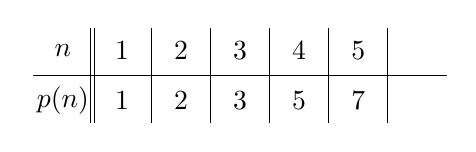
\begin{tikzpicture}[x=0.75cm,y=0.75cm]
\draw (0,0) -- (7.0,0);
\draw (0.96,-0.8) -- (0.96,0.8);
\draw (1.04,-0.8) -- (1.04,0.8);
\draw (2,-0.8) -- (2,0.8);
\draw (3,-0.8) -- (3,0.8);
\draw (4,-0.8) -- (4,0.8);
\draw (5,-0.8) -- (5,0.8);
\draw (6,-0.8) -- (6,0.8);
\node at (0.5,0.42) {$n$};
\node at (0.5,-0.42) {$p(n)$};
\node at (1.5,0.42) {$1$};
\node at (1.5,-0.42) {$1$};
\node at (2.5,0.42) {$2$};
\node at (2.5,-0.42) {$2$};
\node at (3.5,0.42) {$3$};
\node at (3.5,-0.42) {$3$};
\node at (4.5,0.42) {$4$};
\node at (4.5,-0.42) {$5$};
\node at (5.5,0.42) {$5$};
\node at (5.5,-0.42) {$7$};
\end{tikzpicture}
\end{adjustbox}
\end{center}
\begin{equation*}
\sum p(n)t^n=\frac{1}{(1-t)(1-t^2)\ldots}
\end{equation*}
$p(n)=(\text{число классов сопр. элементов }S_n)
=(\text{число непривод. представлений }S_n)$.
\begin{equation*}
p(5n+4)\equiv0\pmod5
\end{equation*}
\begin{equation*}
p(7n+5)\equiv0\pmod7
\end{equation*}

\underline{Зад. Дайсона} (нерешённая), связ. с 1-м сравнением.

$\text{Инвариант}\overset{\mathrm{def}}{=}
(\text{наибольшая часть разб.})-(\text{число частей})$.
\begin{equation*}
8=6+1+1\ \rightsquigarrow\ 3\ (=6-3)
\end{equation*}
\begin{equation*}
8=\underbrace{1+\ldots+1}\ \rightsquigarrow\ -7
\end{equation*}
Остаток [вписано: (инварианта)] от деления на 5 даёт разб. на равные части.

Доказано, но не комбинаторно.

\SourcePage{GELFAND-P001139}{unlabelled}
\underline{21/XI-83 г.}\qquad \underline{Сем. Гельфанда.}

\underline{А.М. Вершик.} (о работах с Керовым).

\Unclear{GELFAND-P001139}{sn-cancellation}{[слева зачёркнут неразборчивый фрагмент]}

$S_n$ — симм. группа.

Рассм. её предст. (неприв.) макс. размерности.

Вопрос: асимптотика
\begin{equation*}
\max_{\pi\in\widehat S_n}\dim\pi\qquad\text{при }n\longrightarrow\infty.
\tag{1}
\end{equation*}
\underline{Утв. 1}
\begin{equation*}
-\lim_n\frac{1}{\sqrt n}\ln\max_\pi\frac{\dim\pi}{\sqrt{n!}}
 =c_0\simeq1{,}2\ldots
\tag{2}
\end{equation*}
или
\begin{equation*}
\max\dim\pi\simeq\sqrt{n!}\,e^{-1{,}2\sqrt n(1+o(1))}
\tag{2'}
\end{equation*}

Реш. получ. с пом. анализа меры Планшереля
(см. ДАН, 1977, 233, $N=6(?)$).

Там асимпт. типичной диагр. Юнга.

\underline{Идея:} имеется предел диаграмм Юнга (и его можно найти!).

Mackay (1976) на ЭВМ считал до $n=81$.

Его гипотеза была о сущ. предст. с $\dfrac{\dim\pi}{\sqrt{n!}}>\dfrac1n$.

Она неверна.

\SourceFigure{GELFAND-P001139}{hook-diagram}{Слева: ступенчатый контур с рядами 5, 3, 1; в верхнем ряду горизонтальный отрезок вправо из второго столбца, из его начала вертикальный отрезок вниз. На горизонтали два утолщения; различить точки и следы пера по оригиналу.}

Размерность предст. по диагр. Юнга.

По $\forall$ точке строится крюк.
\begin{equation*}
\dim=\frac{n!}{\prod(\text{длин крюков})}.
\end{equation*}
\begin{equation*}
\sum\left(\frac{n!}{\prod\ldots}\right)^2=n!
\qquad\text{(следствие теор. теории предст.)}
\end{equation*}

Длины крюков:
\begin{center}
\begin{adjustbox}{max width=\linewidth}
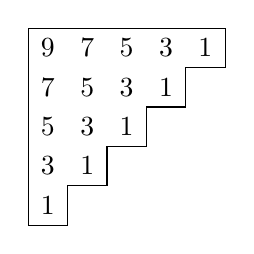
\begin{tikzpicture}[x=0.5cm,y=0.5cm]
\draw (0,0) -- (5,0) -- (5,-1) -- (4,-1) -- (4,-2) -- (3,-2) -- (3,-3) -- (2,-3) -- (2,-4) -- (1,-4) -- (1,-5) -- (0,-5) -- (0,0);
\node at (0.5,-0.5) {$9$};
\node at (1.5,-0.5) {$7$};
\node at (2.5,-0.5) {$5$};
\node at (3.5,-0.5) {$3$};
\node at (4.5,-0.5) {$1$};
\node at (0.5,-1.5) {$7$};
\node at (1.5,-1.5) {$5$};
\node at (2.5,-1.5) {$3$};
\node at (3.5,-1.5) {$1$};
\node at (0.5,-2.5) {$5$};
\node at (1.5,-2.5) {$3$};
\node at (2.5,-2.5) {$1$};
\node at (0.5,-3.5) {$3$};
\node at (1.5,-3.5) {$1$};
\node at (0.5,-4.5) {$1$};
\end{tikzpicture}
\end{adjustbox}
\end{center}
\begin{align*}
\dim&=\frac{15!}{9\cdot7^2\cdot5^3\cdot3^4}\\
&=\frac{15\cdot14\cdot13\cdot12\cdot11\cdot10\cdot9\cdot8\cdot7\cdot6\cdot5\cdot4\cdot3\cdot2}
{9\cdot7\cdot7\cdot5\cdot5\cdot5\cdot3\cdot3\cdot3\cdot3}\\
&=13\cdot11\cdot2^{11}.
\end{align*}
\Unclear{GELFAND-P001139}{factor-cancellations}{[В промежуточной дроби диагональные штрихи сокращения; над $14,12,10,6$ вписаны $2,4,2,2$; над $15$ вписано и зачёркнуто $3$?]}

Или $\dim=$ числу таблиц Юнга с данной схемой;
таблица — возраст. по строкам и столбцам.

Числа $1,2,\ldots,k$, где $k$ — число клеток таблицы.

\begin{center}
\begin{adjustbox}{max width=\linewidth}
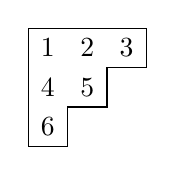
\begin{tikzpicture}[x=0.5cm,y=0.5cm]
\draw (0,0) -- (3,0) -- (3,-1) -- (2,-1) -- (2,-2) -- (1,-2) -- (1,-3) -- (0,-3) -- (0,0);
\node at (0.5,-0.5) {$1$};
\node at (1.5,-0.5) {$2$};
\node at (2.5,-0.5) {$3$};
\node at (0.5,-1.5) {$4$};
\node at (1.5,-1.5) {$5$};
\node at (0.5,-2.5) {$6$};
\end{tikzpicture}
\end{adjustbox}
\end{center}
\underline{16 вариантов} заполнения.

\SourcePage{GELFAND-P001140}{unlabelled}
\underline{Факт:} диагр. представлений [\Unclear{GELFAND-P001140}{top-cancellation}{зачёркнуто: max?}] размерности

[\Unclear{GELFAND-P001140}{left-margin-cancellation}{зачёркнуто на левом поле: $\sqrt n$?}]

\begin{center}
\begin{adjustbox}{max width=\linewidth}
\begin{tikzpicture}[x=1cm,y=1cm]
\draw (0,0) -- (0,1.3) -- (2.3,1.3);
\node[above] at (1.3,1.3) {$4\sqrt n$};
\node[left] at (0,0.65) {$\frac{1}{\sqrt n}$};
\end{tikzpicture}
\end{adjustbox}
\end{center}
нормируем: в пределе кривую.

\SourceFigure{GELFAND-P001140}{limit-curve-diagram}{Наклонные оси с подписями $x$, $\Omega(x)$, горизонтальный и вертикальный отрезки и соединяющая их дуга; тонкий повторный штрих у нижней части дуги неясен.}

$\max$ предст. тоже стремится к этой кривой и типичные тоже.
\begin{equation*}
\Omega(x)=
\begin{cases}
\dfrac{2}{\pi}\bigl(x\arcsin x+\sqrt{1-x^2}\bigr),&|x|\leq 1,\\
|x|,&|x|>1.
\end{cases}
\end{equation*}
\underline{Гистограмма:} по мере Планшереля:
$\dfrac{(\dim\Lambda)^2}{n!}$ — вероятность предст.

Почти все предст. по этой мере стремятся к этой кривой.
Типичные предст. имеют большую флуктуацию.

\underline{Утв. 2.} Макс. предст. — так близко к ней
$\Rightarrow$ счёт на ЭВМ.

Всего $p(n)$ классов сопр. элементов. Их асимптотика
\begin{equation*}
p(n)\simeq\frac{1}{c\sqrt n}\,e^{\frac{2\pi}{\sqrt6}\sqrt n}.
\tag{3}
\end{equation*}
\Unclear{GELFAND-P001140}{partition-prefactor}{в источнике множитель $\frac{1}{c\sqrt n}$}

Это получается из
\begin{equation*}
\sum_n p(n)x^n=\frac{1}{\prod_k(1-x^k)}.
\end{equation*}
([\Unclear{GELFAND-P001140}{integral-cancellation}{зачёркнуто: асимпт.?}] оценивая интегр.)
\Incomplete{GELFAND-P001140}{integral-cancellation-loss}{Не восстановлена отменённая часть слова с а-подобным началом; кандидат «асимпт.?» сохранён, живое «оценивая интегр.» читается отдельно.}
\Unclear{GELFAND-P001140}{integral-live-word-correction}{[Живые слова после зачёркивания: оценивая интегр. Прежнее описание контекста в U028 сохранено как история первой версии; отменённое слово остаётся неопределённым.]}

Радемахер (кн. по аналит. теории чисел) — асимпт. $p(n)$ (полная) —
$\simeq40$ стр.

$p(n)$ — число кривых данной площади.
\begin{center}
\begin{adjustbox}{max width=\linewidth}
\begin{tikzpicture}[x=0.5cm,y=0.5cm]
\draw[->] (0,0) -- (0,4.9);
\draw[->] (0,0) -- (6.3,0);
\draw (0,4) -- (1,4) -- (1,3) -- (3,3) -- (3,2) -- (4,2) -- (4,1) -- (5,1) -- (5,0);
\end{tikzpicture}
\end{adjustbox}
\end{center}

Рассм. таблицы с $n$ клетками и пусть каждая имеет вер. $\dfrac{1}{p(n)}$
(все равновероятны).

Типичная диаграмма? (опять сжимаем в $\sqrt n$ раз)

\underline{Утв. 3.} Получ. кривая (в тех же осях).
\begin{equation*}
e^{-\frac{\pi}{\sqrt6}x}+e^{-\frac{\pi}{\sqrt6}y}=1.
\tag{4}
\end{equation*}
Идея: закон больших чисел (\Unclear{GELFAND-P001140}{random-curve-abbreviation}{теор. случ. кривой / теор. сум. кривой}).

Участки кривой (4) независимы (в слабом смысле).

\SourcePage{GELFAND-P001141}{21}
\underline{Асимпт. Хаара:}
\begin{equation*}
n=n_1+\cdots+n_k.
\end{equation*}
Вероятность пропорц. числу элем. класса. (другая статистика).

Здесь нет предела!

\underline{Статистика Белла.}

$n$ индивид. предметов, разб. на подгруппы

[\Unclear{GELFAND-P001141}{bell-cancellation}{зачёркнуто: разб.?}] Число разбиений.
\Incomplete{GELFAND-P001141}{bell-cancellation-loss}{Не восстановлено окончание отменённой словесной записи с разб-подобным остатком; исходные разб.?/разби… и живое «Число разбиений» сохранены.}

\underline{Характеры.}

$S_\infty$ — финитные подстановки натур. ряда.

$U(\infty)$

Э. Тома (ФРГ) — описал представления $S_\infty$.
1964; Вершик и др. 1981, \Unclear{GELFAND-P001141}{dan-reference}{ФА, 15:4}
\Unclear{GELFAND-P001141}{reference-reading-correction}{[Уточнение записи: ФА, 15:4. Исходная U032 с прежними вариантами сохранена как история первого чтения; отсутствие нового чтения относится к этапу подготовки проекта; ограниченная сверка владельца зафиксирована отдельно.]}

$U(\infty)$ Войкулеску 1976 и Вершик и К$^\circ$ 1982 г. (ДАН)

50-е годы раньше на др. языке (М. Г. Крейн, Гантмахер,
Шёнберг, Карлин — вполне полож. ф-и)

Аналит. зад. — опис. вполне полож. ядр

(\Unclear{GELFAND-P001141}{edrein-name}{Эдрейн / Эдрей} — методами теор. целых ф-й)

\begin{equation*}
\begin{gathered}
U(\infty)\\
\downarrow\\
g
\end{gathered}
\qquad
\chi(g)\text{ — неразложимый характер.}
\end{equation*}
Ф-я:
\begin{enumerate}
\item нормир. $\chi(e)=1$
\item положит. опред.
\item непрерывная.
\end{enumerate}
[Справа, за вертикальной чертой:] $\chi|_{U(n)}$.

$\Rightarrow\chi$ — ф-я на спектре, т. е.
\begin{equation*}
\chi(g)=\prod_{\lambda_i\in\operatorname{Spec}g}\varphi(\lambda_i),
\qquad\varphi(1)=1.
\end{equation*}
Условие на $\varphi$: вполне полож. определённость по Крейну и др.
\begin{equation*}
\varphi(\lambda)=\sum_{n\in\mathbb Z}c_n\lambda^n.
\end{equation*}
\underline{Ответ:} параметры $\gamma^\pm,\alpha_n^\pm,\beta_n^\pm$.
\begin{equation*}
\varphi(z)=
e^{\gamma^+(z-1)+\gamma^-(\bar z-1)}
\prod_k\frac{(1-\beta_k^++\beta_k^+z)}{(1+\alpha_k^+)-\alpha_k^+z}
\cdot
\prod_k\frac{(1-\beta_k^-+\beta_k^-\bar z)}{(1+\alpha_n^-)-\alpha_k^-\bar z}.
\end{equation*}
\Unclear{GELFAND-P001141}{negative-product-index}{[В первом месте знаменателя отрицательного произведения оставлено $\alpha_n^-$; возможное $k$ не подставлено по согласованию индексов. Следующее $\alpha_k^-$ сохранено.]}
\begin{equation*}
\alpha_1^\pm\geq\cdots\geq\alpha_n^\pm\geq\cdots\geq0,
\qquad\gamma^\pm\geq0,
\end{equation*}
\begin{equation*}
\beta_1^\pm\geq\cdots\geq\beta_n^\pm\geq\cdots\geq0,
\end{equation*}
\begin{equation*}
\sum\alpha_k^++\alpha_k^-+\beta_k^++\beta_k^-<\infty,
\end{equation*}
\begin{equation*}
\beta_1^++\beta_1^-\leq1.
\end{equation*}

\SourcePage{GELFAND-P001142}{unlabelled}
$S_\infty$ — разница небольшая, но аналит. ф-и (без отриц. степеней).
\Unclear{GELFAND-P001142}{small-mark-under-bez}{[Под «без» виден небольшой переправленный/зачёркнутый штрих; прежнее содержание не установлено. Читаемое «без» сохранено; отдельная потеря слова не утверждается.]}

$\alpha_j,\beta_j$ — предельные параметры диаграмм Юнга.

Якоби \Unclear{GELFAND-P001142}{jacobi-caption}{симв. / смысл}:
\begin{equation*}
\frac{
\begin{vmatrix}
x_1^{\lambda_1}&x_2^{\lambda_1}&\cdots&x_n^{\lambda_n}\\
x_1^{\lambda_2+1}&x_2^{\lambda_2+1}&\cdots&x_n^{\lambda_2+1}\\
\vdots&\vdots&&\vdots
\end{vmatrix}
}{
\begin{vmatrix}
1&\cdots&\cdots&1\\
x_1&x_2&\cdots&x_n\\
x_1^2&x_2^2&\cdots&x_n^2\\
\vdots&\vdots&&\vdots\\
x_1^{n-1}&\cdots&\cdots&x_n^{n-1}
\end{vmatrix}
},
\qquad
\lambda_1\leq\lambda_2\leq\cdots\leq\lambda_n.
\tag{5}
\end{equation*}
\Unclear{GELFAND-P001142}{numerator-indices}{справа в первой строке написано $x_n^{\lambda_n}$; возможная описка источника}

Пусть сущ. $\displaystyle\lim_{n\to\infty}\frac{\lambda_k^{(n)}}{n}=\alpha_k$
$\Rightarrow$ сущ. предел $\det$ (5) и он есть
производ. ф-я характеров.

\underline{Утв.} Пусть $|x_i|=1$ и начиная с нек-рого они $=1$.

Мива, Джимбо: по каждой диагр. — дифф. оператор.

\underline{$K$-функтор:}

\underline{Зап. сем. ЛОМИ,} [\Unclear{GELFAND-P001142}{lomi-reference-cancellation}{зачёркнуто: № / число}] \underline{т. 123}

[Короткая разделительная черта.]

$K^0(S_\infty)$ строятся по проект. модулям над $\mathbb C(S_\infty)$

(конечно порожд. модули явл. прямыми слагаемыми).

$K^0(S_n)$ — аддитивная группа характеров.
\Unclear{GELFAND-P001142}{additive-group-word-correction}{[Написано: аддитивная группа характеров; слово не заменяется математически эквивалентным «абелевая».]}

\underline{Теор.:}
\begin{equation*}
\underset{n\to\infty}{\underrightarrow{\lim}}K^0(S_n)
=K^0(S_\infty)=A/\{s_1-1\}.
\end{equation*}
\Unclear{GELFAND-P001142}{ideal-subscript}{нижний знак у $s$: $1$ / $i$}

[Под $A$:] $\sigma_1\oplus\sigma_2\oplus\cdots$.

[Под $K^0(S_\infty)$, соединено короткой вертикальной чертой:]
это уже не группа характеров.

(вложение — с пом. индуцированных представлений).

[Справа:]
\begin{equation*}
\sigma_n\times\sigma_m\subset\sigma_{n+m}.
\end{equation*}

Описание полож. элементов? В терминах дифф. опер даётся.

Положительность — полож. комбинации характеров.

Конус полож. эл. устроен нетривиально.
\SourcePage{GELFAND-P001143}{unlabelled}

\underline{28/$\overline{\underline{\mathrm{XI}}}$-83 г.}
\qquad
\underline{\underline{Сем. Гельфанда.}}

\underline{И.М.Г.}\qquad Неясно, что такое $\infty$-мерное пр-во.

Повт. Вершика

\begin{center}
\begin{adjustbox}{max width=\linewidth}
\begin{tikzpicture}
\draw (0,0) -- (0.6,0);
\draw (0.85,-0.04) -- (0.88,0.09);
\draw (1.15,0) -- (2.1,0);
\end{tikzpicture}
\end{adjustbox}
\end{center}

\underline{А. Мигдал.}\quad
[Зачёркнуто: \Unclear{GELFAND-P001143}{cancelled-intro-word}{неразборчивое слово}.]
Интересен случай откл. от ЦПТ (гаусс. пред. теор.)

\begin{equation*}
\int d\vec{\tau}\,\delta(1-\vec{\tau}^{\,2})\,
e^{i\bar{k}\bar{\tau}}\sim J_n(k)
\tag{1}
\end{equation*}

Отсюда получ. асимптотика Бесселевых ф-й

Пусть Большое число измерений!

Если не менять $k$, то будет
$\begin{gathered}[t]
\text{ЦПТ}\\
\downarrow\\
\text{стремится к гаусс. распред.}
\end{gathered}
\qquad
\begin{gathered}[t]
(n\to\infty)\\
k\text{ фиксир.}
\end{gathered}$

\underline{Д-во:}\qquad $\delta$ заменяем на $\int$ Фурье; интегр. по $\tau$

\begin{equation*}
\int d\alpha\int d\vec{\tau}\,
e^{\alpha(1-\tau^2)+ik\tau}
\end{equation*}

[После первого знака $\int$ перед $d\alpha$ зачёркнуто:
\Unclear{GELFAND-P001143}{cancelled-fourier-factor}{неразборчивый фрагмент формулы}.]

$\alpha\in i\mathbb{R}\qquad\Vert$\quad
интегр. по $\tau$ считаем $\Rightarrow$ гаусс. распред.

\SourcePage{GELFAND-P001144}{unlabelled}

Получим
\begin{equation*}
\int\frac{d\alpha}{2\pi i}\,
\alpha^{-n/2}e^{\alpha-\frac{k^2}{4\alpha}}
\end{equation*}

Берем $\underline{k\sim n}$ !!
\qquad заменяем $\alpha$ на $n\alpha$ в интеграле

[Зачёркнуто: $\alpha\sim n$,
\Unclear{GELFAND-P001144}{cancelled-scaling-line}{неразборчивые знаки и слово}.]

\begin{equation*}
\int\frac{d\alpha}{2\pi i}\,
\alpha^{-\frac n2}e^{n\alpha-\frac{k^2}{4\alpha n}}
\end{equation*}

$\alpha$ слабо флуктуирует $\Rightarrow$ заменяем его на const при малом $k$

$n$ велико, $k\sim n$ $\Rightarrow$ получ. какой-то $\arcsin$.

\underline{Аналог. задача возник. для}

\underline{Интеграла Фурье по унит. группе}

\begin{equation*}
\int du\,\exp\bigl(\beta\operatorname{tr}(\bar n u+u^+n)\bigr),
\qquad u^+u=I
\tag{2}
\end{equation*}

($n,\bar n$ — пост. матрицы)

[$\bar n$ вписано над строкой со стрелкой к месту после $n$.]

\Unclear{GELFAND-P001144}{matrix-parameter}{В (2), пояснении и двух матричных интегралах ниже: $n$ или $\eta$.}

Нетрив. асимптотика больших групп (асимптотики нет)

Снова.

\begin{equation*}
\int d\vec{\tau}\,\delta(1-\vec{\tau}^{\,2})e^{i\vec{k}\vec{\tau}}
\qquad
2\pi i\,\delta(x)=\int_{-i\infty}^{i\infty}e^{\alpha x}\,d\alpha
\end{equation*}

$\Vert$

[Перед $\frac1{2\pi i}$ зачёркнуто:
\Unclear{GELFAND-P001144}{cancelled-integral-prefix}{$\int d\alpha$?}.]

\begin{equation*}
\begin{aligned}
&\frac1{2\pi i}\,n\int d\alpha\int d\vec{\tau}\,
e^{n\alpha(1-\vec{\tau}^{\,2})+i\vec{k}\vec{\tau}}={}\\
&=\int d\alpha\,
\exp\left(-\frac n2\ln\alpha+n\alpha-\frac{k^2}{4\pi\alpha}\right)
\end{aligned}
\end{equation*}

\Unclear{GELFAND-P001144}{gaussian-denominator}{В последнем знаменателе: $4\pi\alpha$ или $4n\alpha$.}

$k\sim n\Rightarrow$ применим метод перевала

Энтропия: $n$-кратный интеграл с экспонентой, сод. $n$, равен $e^{n(\ldots)}$

$\Rightarrow\ln$ числа сост. $=\ln$ интеграла $\sim n$.

Попробуем для (2) — заменяем его на
\qquad $u\in U(N)$

\begin{equation*}
\int
\underbrace{du\,du^+\,
\delta\bigl(\overbrace{I-u^+u}^{\text{матрица}}\bigr)}
_{\text{инв. мера}\ \Rightarrow\ \substack{\text{мера}\\\text{Хаара}}}
\exp\bigl(N\beta\operatorname{tr}(\bar n u+u^+n)\bigr).
\end{equation*}

[После знака $\int$ перед $du$ зачёркнуто:
\Unclear{GELFAND-P001144}{cancelled-haar-prefix}{неразборчивый знак}.]

[После $du^+$ перед $\delta$ зачёркнуто:
\Unclear{GELFAND-P001144}{cancelled-haar-dalpha}{$d\alpha$?}.]

[$N$ вписано над $\beta$; две пунктирные стрелки направлены к месту перед $\beta$.]

\begin{equation*}
\int du\,du^+\,d\alpha\,
\exp\bigl(N\operatorname{tr}(\alpha-u^+u\alpha)
+N\beta\operatorname{tr}(\bar n u+u^+n)\bigr)
\end{equation*}

\SourcePage{GELFAND-P001145}{28}

$\int d\alpha$ не удаётся взять методом перевала.

Энтропия, связ. с $\alpha$, того же порядка:

$N^2$ членов и $N^2$ интегралов $\Rightarrow$ каждый интеграл $\sim1$ и нет асимптотики

(у 1-мерн. интеграла)

(\underline{Правило} \underline{стат.} \underline{физ.}:

Многок. интеграл $\sim e^k$, где $k$ — число измерений)

\begin{center}
\begin{adjustbox}{max width=\linewidth}
\begin{tikzpicture}
\draw (0,0) -- (1,0);
\fill (1.35,0) circle (0.025);
\draw (1.65,0) -- (2.7,0);
\end{tikzpicture}
\end{adjustbox}
\end{center}

\underline{Амбула.}

Рассм. задача

\begin{equation*}
\int dA\,\exp\bigl(+N\beta\operatorname{Sp}(V(A))\bigr)\,
\operatorname{Sp}(e^{At})
\tag{3}
\end{equation*}

$A$ — эрмитовы матрицы (ал. группы $SU(N)$)
\qquad $A^+=-A$.

[Над строкой перед «эрмитовы» вписано «косо» со знаком вставки.]

\begin{equation*}
\underset{\text{— полином}}{V(A)}
=v_1A+\ldots+v_nA^n,\qquad v_j\text{ — числа}
\end{equation*}

\Unclear{GELFAND-P001145}{polynomial-coefficients}{Знак коэффициентов: $v$ или $\nu$.}

\begin{equation*}
\Psi(t)=
\frac{(3)}
{\int dA\,\exp\bigl(-N\beta\operatorname{Sp}(V(A))\bigr)}
\tag{4}
\end{equation*}

(производ. ф-я для моментов)

[В знаменателе после $N\beta$ перед $\operatorname{Sp}$ зачёркнуто:
\Unclear{GELFAND-P001145}{cancelled-normalizing-factor}{неразборчивый знак}.]

\Unclear{GELFAND-P001145}{exponential-signs}{В (3) виден $+N\beta$, в (4) виден $-N\beta$; несогласование знаков не разрешено.}

Более сложный объект: среднее Вильсона

\begin{equation*}
\operatorname{Sp}\,T\exp\left(\int_C A_\alpha\,dx_\alpha\right).
\qquad (T\text{ — матрица})
\end{equation*}

[Зачёркнуто:
\Unclear{GELFAND-P001145}{cancelled-wilson-word}{неразборчивое слово}.]

Рассм.

\begin{equation*}
0=\int dA\,\frac{\partial}{\partial A_{ij}}
\left[e^{At}\exp\bigl(N\beta\operatorname{Sp}V(A)\bigr)\right]
\tag{5}
\end{equation*}

\begin{equation*}
\sum_{i,j}\frac{\partial}{\partial A_{ij}}\,
\underset{\substack{\Vert\\\prod(1+A\,dt)}}{(e^{At})_{ij}}
=\int_0^t d\tau\,\operatorname{Sp}(e^{A\tau})
\operatorname{Sp}(e^{A(t-\tau)})
\end{equation*}

и диффер. $t$ сомножитель

(то, что впереди — собир. в exp;

то, что позади — тоже собир. в exp).

Более общ.:

[В начале (6) перед $\frac{\partial}{\partial A_{ij}}$ зачёркнуто:
\Unclear{GELFAND-P001145}{cancelled-eq6-sum}{$\sum_{i,j}$?}.]

\begin{equation*}
\frac{\partial}{\partial A_{ij}}(e^{At})_{k\ell}
=\int_0^t d\tau\,(e^{A\tau})_{ki}\cdot(e^{A(t-\tau)})_{j\ell}
\tag{6}
\end{equation*}

[В показателе первого правого экспоненциального множителя последний знак записан поверх другого:
\Unclear{GELFAND-P001145}{eq6-exponent-overwrite}{неразборчивый первоначальный знак под $\tau$}.]

\begin{equation*}
\frac{\partial}{\partial A_{ij}}\operatorname{Sp}V(A)
=(V'(A))_{ji}
\tag{7}
\end{equation*}

($V$ — полином)

Пользуясь (6), (7), дифференцируем в (5).

\SourcePage{GELFAND-P001146}{unlabelled}
Вычисляется
\begin{equation}
\frac{\int dA\,\exp(N\beta\operatorname{Sp}V(A))\operatorname{Sp}(e^{At})/N}
{\int dA\,\exp(N\beta\operatorname{Sp}V(A))}
\overset{\Unclear{GELFAND-P001146}{definition-abbreviation}{\mathrm{df}}}{=}
\left\langle\frac{\operatorname{Sp}e^{At}}{N}\right\rangle
\tag{8}
\end{equation}
Из (5)–(7) находим
\begin{equation}
0=\left\langle\left(\int_0^t d\tau\,\operatorname{Sp}e^{A\tau}
\operatorname{Sp}e^{A(t-\tau)}\right)
+N\beta\operatorname{Sp}(V'(A)e^{At})\right\rangle
\tag{9}
\end{equation}
\begin{equation*}
N\beta\quad\text{[зачёркнуто: }\Unclear{GELFAND-P001146}{cancelled-trace}{\operatorname{Sp}\text{?}}\text{]}\quad
V'\left(\frac{\partial}{\partial t}\right)\operatorname{Sp}(e^{At})
\end{equation*}
\begin{equation*}
\operatorname{Sp}\mapsto\frac{\operatorname{Sp}}{N}
\qquad\text{(среднее соб. значений)}
\end{equation*}
[Зачёркнуто: $\operatorname{Sp}(AB)$.]
\begin{equation*}
\langle\operatorname{Sp}A\cdot\operatorname{Sp}B\rangle
\sim\Unclear{GELFAND-P001146}{factorization-expression}{\langle\operatorname{Sp}(A\cdot B)\rangle}
\end{equation*}
(статист. факт.)

Получаем
\begin{equation}
0=\beta V'\left(\frac{\partial}{\partial t}\right)\Psi(t)
+\int_0^t d\tau\,\Psi(\tau)\Psi(t-\tau)
\tag{10}
\end{equation}
Решается \Unclear{GELFAND-P001146}{fourier-abbreviation}{пробр.} Фурье (Лапласа)
\begin{equation}
\beta V'(\omega)\Psi(\omega)+\Psi^2(\omega)=K(\omega)
\tag{11}
\end{equation}
[Под $K(\omega)$ скобка со штрихом к подписи: из интегр. по частям.]

Отсюда
\begin{equation}
\Psi=-\frac{\beta}{2}V'+\sqrt{\frac{\beta^2}{4}V'^{2}\Unclear{GELFAND-P001146}{quadratic-sign}{-K(\omega)}}
\tag{12}
\end{equation}
$K(\omega)$ выбир. так, чтобы корень почти извлекался.

Для $\int$ по группе — аналогично. Ур-е выглядит так:
\begin{equation}
\int du\,[F(u)-F(u(1+\delta))]=0
\qquad\text{(усл. правоинвар. меры Хаара)}
\tag{13}
\end{equation}
\begin{equation*}
\int du\,\left(\frac{\partial F}{\partial u_{ij}}u_{jk}\right)=0
\end{equation*}
и т. д.

Можно при произвольном $N$ и т. д. $\Rightarrow$ отсюда алгоритм для нахожд.
ряда по степеням $1/N$.

Теор. поля — аналог. ур-я, но функциональные.

[Внизу отдельный знак: \Unclear{GELFAND-P001146}{bottom-isolated-mark}{$\int$ [перечёркнуто?]}.]

\SourcePage{GELFAND-P001147}{29}
\begin{equation}
\frac{\int e^{N\beta\operatorname{Sp}V(A)}\frac1N\operatorname{Sp}e^{At}\,dA}
{\int e^{N\beta\operatorname{Sp}V(A)}\,dA}
=\Psi_N(t)=\Psi(t)+\frac1{N^2}\Psi_1(t)+\cdots
\tag{14}
\end{equation}
(асимпт. разл. по $1/N$)

Рассм. ещё
\begin{equation}
\left\langle\frac{\operatorname{Sp}e^{At}}N\right\rangle
=\frac{\int dA\,\exp(N\beta\operatorname{Sp}V(A)+\Unclear{GELFAND-P001147}{source-coupling-numerator}{\int J(t)\,dt})\operatorname{Sp}e^{At}\text{[зачёркнуто: }\Unclear{GELFAND-P001147}{cancelled-numerator-symbol}{\text{неразборчиво}}\text{]}/N}
{\int dA\,\exp(N\beta\operatorname{Sp}V(A)+\Unclear{GELFAND-P001147}{source-coupling-denominator}{\int dt\,J(t)\operatorname{Sp}(e^{At})}}
\tag{15}
\end{equation}
Получается уравнение: (вроде ур. Фурье)
\begin{equation}
\begin{aligned}
\beta V'\left(\frac{\partial}{\partial t}\right)\Psi(t,J)
&=\Unclear{GELFAND-P001147}{loop-equation-sign}{\int_0^t d\tau\,\Psi(\tau)\Psi(t-\tau)}+{}\\
&\quad+\Unclear{GELFAND-P001147}{loop-equation-coefficient}{\frac1N}
\left\{\int_0^t d\tau\,\frac{\delta\Psi(t-\tau)}{\delta J(\tau)}
+\int_0^\infty d\tau\,J(\tau)\Psi(t+\tau)\right\}
\end{aligned}
\tag{16}
\end{equation}
\underline{Теор. поля.}
\begin{equation*}
V(A)=F_{\mu\nu}^2,\qquad V'(A)\equiv\nabla_\mu F_{\mu\nu}
\end{equation*}
\begin{equation*}
V'\left(\frac{\partial}{\partial t}\right)\mapsto
\int_0^1 ds_1\int_{s_1-0}^{s_1+0}ds_2\,
\frac{\delta^2}{\delta x_\mu(s_1)\delta x_\nu(s_2)}.
\end{equation*}

\underline{Вигман П.}

\underline{Точное реш. главного кирального поля в 2-мерн. пр-ве}

(совм. с Поляковым по его программе, предложенной 10 лет назад)
\begin{equation}
\int e^{-\frac1{\Unclear{GELFAND-P001147}{chiral-coupling-denominator}{T}}\int d^2x\,\operatorname{tr}(V^{-1}\partial_\mu V)^2}\,
\Unclear{GELFAND-P001147}{chiral-field-letter}{\mathcal D U}
\tag{1}
\end{equation}
$V=V(x),\quad x=(x^1,x^2)$

[Под $x^1,x^2$ зачёркнуты нижние знаки: \Unclear{GELFAND-P001147}{cancelled-coordinate-indices}{неразборчиво}.]

(от $n=2$ к $n=4$ есть идеи А. Б. Замолодчикова, пока не приведшие к успеху)

[Под «А. Б.» вписано: Александр.]

Что описывает? $\pi$ и $K$-мезоны (если в $R^4$)
\Unclear{GELFAND-P001147}{mark-after-mesons}{[знак, похожий на перечёркнутое $\int$]}

$(1+1)$ КТП или эквив. 2-мерные стат. задачи

[Под $(1+1)$: и; ниже: $(2+0)$.]

В посл. время решено много 2-мерных квантовых моделей. Это одна из них.

Глоссарий необходимых терминов из теории поля
\begin{enumerate}
\item Группа перенормировок
\item Асимптотическая свобода
\item Квантовая аномалия аксиального тока.
\item Анзац Бете (Bethe) $\cong$ метод квантовой обратной задачи рассеяния
\item $\operatorname{Det}(i\partial_\mu\gamma^\mu+A_\mu^{(x)}\gamma^\mu)=W\{A\},\qquad A_\mu=\sum_a A_\mu^aX^a$
\end{enumerate}

\SourcePage{GELFAND-P001148}{unlabelled}
\begin{equation*}
A_+=a^{-1}\partial_+a,\qquad A_-=b^{-1}\partial_-b.
\end{equation*}
\begin{equation*}
g=ab^{-1}
\end{equation*}
\begin{equation*}
\mathcal A_\mu=g^{-1}\partial_\mu g
\end{equation*}
\begin{equation*}
W\{A\}=\frac12\int\operatorname{tr}\mathcal A_\mu^2\,d^2x
+\Unclear{GELFAND-P001148}{cubic-term-coefficient}{\frac{i}{8\pi}}\int_Qd^3\xi\,\varepsilon^{ABC}\mathcal A_A\mathcal A_B\mathcal A_C
\end{equation*}
\begin{equation*}
\partial Q=S^2,
\end{equation*}

\SourcePage{GELFAND-P001149}{unlabelled}
\noindent\underline{5/XII--83 г.}\quad\underline{Сем. Гельфанда.}

\noindent\underline{\underline{П. Вигман.}}

Что нужно знать?

1. \underline{Анзац Бете.} — осн. \Unclear{GELFAND-P001149}{upper-list-one}{иде. / идея / идеи}. Остальные вопр.

[Зачёркнуто: 2. \Unclear{GELFAND-P001149}{upper-list-cancelled}{Перенормируемость.}]

2. Перенормируемость.

3. Критические явления.

4. Асимптотическая свобода.

5. Калибровочные теории: аксиальная аномалия,

[В начале следующей строки зачёркнуто: \Unclear{GELFAND-P001149}{middle-list-cancelled-number}{неразборчивое обозначение}.]
Инстантоны и топология, $\theta$-вакуум.

6. Теория струн, которая пока не существует, петля Вильсона, минимальные поверхности, статистика случайных поверхностей.

7. Алгебра Вирасоро.

8. \underline{Ф. Тв. Тела}: есть \underline{локализация Андерсона}
(пока не \Unclear{GELFAND-P001149}{middle-localization-ending}{понятная / понятая}).

[Под словом «локализация»: (явление).]

Главное киральное поле в 2-х измерениях.
\begin{equation*}
(1)\qquad S=\frac{1}{2\lambda}\int d^2x\,\operatorname{tr}(g^{-1}\partial_\mu g)^2,
\qquad g\in G,\quad
\begin{gathered}g=g(x),\\\mu=0,1.\end{gathered}
\end{equation*}
[Справа: Интегрир. в [зачёркнуто: \Unclear{GELFAND-P001149}{middle-right-cancelled}{неразборчивое обозначение}] класс. области. \underline{Оказ., что и в квант. тоже.}]

Квант. интегрируемость: возможность вычислить интеграл
\begin{equation*}
(2)\qquad Z=\int e^{-S}\,Dg.
\end{equation*}
или диагонализация соотв. гамильтониана

Будут станд. вычисления по поводу этого $\longrightarrow$ анзац Бете.

Надо знать соб. состояние (пусть не основное). Для бозонного поля такое неизвестно. Нужно сделать след. шаг:

(3) \underline{Утв.}\quad\underline{Теория экв. фермионной теории с лагранжианом}
\begin{equation*}
(4)\qquad \mathcal L=\bar\psi i\hat\partial\psi+\lambda j_\mu^a j_a^\mu,
\qquad S=\int\mathcal L\,d^2x
\end{equation*}
\begin{equation*}
\psi=\begin{pmatrix}\psi_R\\\psi_L\end{pmatrix}
\quad\text{(дираковский спинор)},\qquad
\text{преобр. согл. }O(2)
\quad\text{(гр. Лоренца в 2-мер. случае)}
\end{equation*}
\begin{equation*}
\hat\partial=\gamma_\mu\partial^\mu,
\qquad \{\gamma_\mu,\gamma_\nu\}=2\delta_{\mu\nu}
\end{equation*}
[Под $\hat\partial$: — опер. Дирака $(\mu=0,1)$.]
\begin{equation*}
\gamma_0,\gamma_1
\end{equation*}

\SourcePage{GELFAND-P001150}{36}
Изотопич. значки
\begin{equation*}
\begin{gathered}
\alpha=1,\ldots,N\quad\text{— цвет.}\\
f\quad\text{— запах = аромат (flavour)}\\
f=1,\ldots,N_f
\end{gathered}
\qquad (g\in SU(N))
\end{equation*}
\begin{equation*}
(5)\qquad j_\mu^a=\sum_f\bar\psi_f^\alpha\gamma_\mu X_{\alpha\beta}^a\psi_f^\beta,
\qquad X^a\text{ — генераторы группы }SU(N)
\end{equation*}
Через токи строится взаимодействие.

(6) \underline{Утв.} При $N_f\longrightarrow\infty$ эти теории эквивалентны.

(теория (4) переходит в теорию (1))

Цветные гр. должны совпасть.

Имеется левая и правая инвариантность.
\begin{equation*}
g\longrightarrow gG\quad\text{и т. д.; группа }G\times G
\end{equation*}
У теории (4):\quad $\underline{G\times F}$

Правая инвар. отсутствует и восстанавл. при $\infty$ числе flavour'ов.

У (4) есть соб. вектор — \underline{вакуум $|0\rangle$}: $\Psi|0\rangle=0$

[К $\Psi$ проведена линия с подписью: опер. [зачёркнуто: \Unclear{GELFAND-P001150}{middle-vacuum-cancelled}{рожд.}] уничтож.]

(1) описывает 2-мерные \Unclear{GELFAND-P001150}{middle-magnetic-correction}{магнит… [окончание зачёркнуто; ниже вписано: ные]} [вписано ниже: теор.], но
такие зад. похожи на 4-мерные калибр. теории (есть соображения, но пока словесные).

\underline{Д-во эквивалентности.}

[Слева под заголовком зачёркнуто: \Unclear{GELFAND-P001150}{middle-proof-cancelled-number}{неразборчивое обозначение}.]
\begin{equation*}
(7)\qquad (4)\Longrightarrow\bar\psi(i\partial_\mu\gamma^\mu+A_\mu)\psi+\frac{A_\mu^2}{2\lambda}
\end{equation*}
\Unclear{GELFAND-P001150}{lower-equation-seven}{При $A_\mu$ множитель $\gamma^\mu$ в этой строке не записан.}
[Справа: $A_\mu\bar\psi\gamma_\mu\psi=A_\mu j^\mu$.]

из равенства
\begin{equation*}
(8)\qquad e^{\lambda j_\mu j_\mu}
=\left(\int e^{A_\mu j_\mu+\frac{A_\mu^2}{2\lambda}}\,DA_\mu\right)
\Big/\left(\int e^{\frac{1}{2\lambda}A^2}\,DA\right)
\end{equation*}
\Unclear{GELFAND-P001150}{lower-gaussian-signs}{Знаки и коэффициенты равенства воспроизведены как написаны.}

(гауссов. интеграл с промеж. полем)
\begin{equation*}
(9)\qquad \int e^{S(\psi)}\,D\psi=\int e^{S(\psi,A)}\,DA\,D\psi
\end{equation*}
\Unclear{GELFAND-P001150}{lower-exponential-signs}{В обоих показателях (9) перед $S$ нет минуса.}

Индекс $f$ опускается для простоты.

(Иногда наз. ф-лой Стратоновича--Хаббарда)

[Перед следующей строкой зачёркнуто: \Unclear{GELFAND-P001150}{bottom-cancelled-number}{неразборчивое обозначение}.]
\begin{equation*}
\int_{D\psi}=\frac{A_\mu^2}{2\lambda}+\overset{N_f}{\ln}\operatorname{Det}(i\partial_\mu\gamma^\mu+A_\mu\gamma^\mu)
\end{equation*}
[Под интегралом: в (9). Над $\ln\operatorname{Det}$ вписано $N_f$ с обводящей линией.]
\Unclear{GELFAND-P001150}{bottom-determinant-shorthand}{Левая часть сокращённой записи и положение вставки $N_f$ сохранены; их точное математическое значение не восстановлено.}
\begin{equation*}
(10)\qquad S(\psi,A)=\int d^2x\left\{\sum_{f=1}^{N_f}\bar\psi_f(i\partial_\mu\gamma^\mu+\gamma^\mu A_\mu)\psi_f+\frac{A^2}{2\lambda}\,\mu\right\}
\end{equation*}
\Unclear{GELFAND-P001150}{bottom-equation-ten-index}{Буква $\mu$ написана справа от дроби; возможно, это вынесенный индекс при $A^2$.}

\SourcePage{GELFAND-P001151}{unlabelled}
Получается
\begin{equation*}
(11)\qquad S\{A\}=\int\left[\frac{A_\mu^2}{2\lambda}+N_f\ln\operatorname{Det}(i\partial_\mu\gamma^\mu+A_\mu\gamma^\mu)\right]d^2x
\end{equation*}
Надо вычислить \Unclear{GELFAND-P001151}{upper-looped-mark}{петлеобразный знак; возможно, зачёркнутый интеграл}
\begin{equation*}
(12)\qquad \int e^{-S(A)}\,DA_\mu
\end{equation*}
[Справа: $A_\mu$ уже бозонное поле.]

и затем\quad $\underline{N_f\longrightarrow\infty}$.

$\Longrightarrow$ в пределе будут влиять траект., где $\min\ln\operatorname{Det}$

Возникает связь на поля $A_\mu$: а именно, $\min$ на полях
\begin{equation*}
(13)\qquad \underline{A_\mu=g^{-1}\partial_\mu g}
\end{equation*}
(чисто калибр. поле); это в точности те, на к-рых $F_{\mu\nu}=0$
\begin{equation*}
(14)\qquad \lim_{N_f\to\infty}\int e^{-S(A)}\,DA_\mu
=\int e^{-S(A_\mu)}\delta(F_{\mu\nu})\,DA_\mu
\end{equation*}
\begin{equation*}
F_{\mu\nu}=\partial_\nu A_\mu-\partial_\mu A_\nu+[A_\mu,A_\nu]
\end{equation*}
\Unclear{GELFAND-P001151}{middle-curvature-signs}{Порядок индексов и знак коммутатора сохранены; согласование с (13) требует проверки.}

Зад. с конечн. числом ароматов тоже интегрируема. Она и интегрируется,
а затем пред. переход.

Задача о классич. интегр. $\sim$ [зачёркнуто: \Unclear{GELFAND-P001151}{middle-classical-cancelled}{экв.}]
[вписано сверху: интегр.] кир. поля с доб. члена Весса--Зумино.

\underline{Калиб. преобр.:}
\begin{equation*}
(15)\qquad A_\mu\longrightarrow U^{-1}A_\mu U+U^{-1}\partial_\mu U
\end{equation*}
$(13)\sim0$ при этом, или $F_{\mu\nu}=0$ на (13).

$\det$ — калибр. инвариантен; все соб. знач. опер. Дирака калибр. инвар.
\begin{equation*}
(i\partial_\mu\gamma^\mu+A_\mu\gamma^\mu)\Psi=\lambda\Psi
\end{equation*}
Калиб. преобр. надо сверш. над $A_\mu$ и одновр. над $\Psi$

(16)\quad\underline{$\min$ — на полях, калибр. экв. $0$.}

Пусть для простоты абелево:
\begin{equation*}
(17)\qquad A_\mu=\partial_\mu\varphi+\epsilon_{\mu\nu}\partial_\nu\Phi
\end{equation*}
Преобр.\quad $A_\mu\longmapsto\partial_\mu\varphi+A_\mu$

В этом случае:
\begin{equation*}
(18)\qquad \ln\operatorname{Det}(i\partial_\mu\gamma^\mu+A_\mu\gamma^\mu)
=\int d^2x\,(\partial_\mu\Phi)^2\qquad\text{(Швингер, 1961)}
\end{equation*}
Отсюда вариация $\det>0$, если есть $\Phi$.

Мораль: $A_\mu=\partial_\mu\varphi$ и т. д.

\begin{center}
\rule{1.5cm}{0.3pt}\quad$\bullet$\quad\rule{1.5cm}{0.3pt}
\end{center}

\SourcePage{GELFAND-P001152}{37}
\underline{Метод анзаца Бете.}

Упростим, выкинув ароматы (оставим 1), а цвета $SU(2)$.
[Над «оставим 1» вписано: $N_f=1$.]
Будет \underline{нерелятивистская} задача. (для простоты)

О диагонализации след. фермионного гамильтониана.

\Unclear{GELFAND-P001152}{eq19-cancelled}{[Перед формулой (19) зачёркнут знак: $\mathcal{H}$?]}
\begin{equation}
\mathcal{L}=\bar{\psi}\,i\hat{\partial}\psi
+\lambda\bar{\psi}\gamma_\mu\bar{\sigma}\psi
\bar{\psi}\gamma_\mu\bar{\sigma}\psi
\tag{19}
\end{equation}

$\bar{\sigma}$ — матр. Паули (гр. $SU(2)$), действ. на цветов. индекс.

Плотность гамильтониана: (нерелятив.):
\begin{equation}
\mathcal{H}=\sum_{\sigma=\pm}\psi_\sigma^+
\frac{d^2}{dx^2}\psi_\sigma
+\lambda(\psi_\sigma^+\psi_\sigma)
(\psi_{\sigma'}^+\psi_{\sigma'})
\tag{20}
\end{equation}
\Unclear{GELFAND-P001152}{eq20-kinetic-sign}{[Знак кинетического члена сохранён по рукописи.]}
[Справа от (20):] (гам. в предст. вторичного квантования)

$\sigma$ — спин.

Спектр $\mathcal{H}$ уже ограничен снизу (в отличие от (19)) — это фактич.
регуляризация (19) и с точн. до неё задачи эквивалентны.

$\psi_\sigma=\psi_\sigma(x)$.

Гамильтониан:
\begin{equation}
H=\int\mathcal{H}\,dx
\qquad
\psi_\sigma=\begin{pmatrix}\psi_+\\\psi_-\end{pmatrix}.
\tag{21}
\end{equation}

$\psi$ — фермионное поле, т.е.
\begin{equation}
\{\psi_\sigma^+(x),\psi_{\sigma'}(y)\}
=\delta(x-y)\delta_{\sigma\sigma'}
\tag{22}
\end{equation}

\underline{Задача:} найти все соб. числа и соб. ф-и гамильтониана $H$.
\begin{equation}
H\Phi=\lambda\Phi.
\tag{23}
\end{equation}
\begin{equation}
N=\int\psi^+\psi\,dx
\tag{24}
\end{equation}
— число частиц. (коммутирует с $H$)

Сист. опис. волн. ф-й
\begin{equation*}
\Phi(x_1,\ldots,x_N,\sigma_1,\ldots,\sigma_N)
\end{equation*}
\begin{equation}
S^z=\sum_\sigma\int\sigma\psi_\sigma^+\psi_\sigma\,dx
\tag{25}
\end{equation}

Рассм. предст. гр. перестановок (пар $(x_j,\sigma_j)$)

Фермионы — антисимметр.

% Young diagram: original pixels x=1182..1486, y=2837..3022.
% The small gaps in the first inner horizontal and lower right strokes are retained.
\begin{center}
\begin{adjustbox}{max width=\linewidth}
\begin{tikzpicture}[x=0.35cm,y=0.35cm]
\draw (0,0)--(5,0)--(5,-1)--(3,-1)--(3,-2)--(2,-2);
\draw (2,-2)--(2,-2.9);
\draw (2,-3)--(0,-3)--(0,0);
\draw (1,0)--(1,-3);
\draw (2,0)--(2,-2);
\draw (3,0)--(3,-1);
\draw (4,0)--(4,-1);
\draw (0,-1)--(2.78,-0.92);
\draw (0,-2)--(3,-2);
\node[anchor=west] at (5.7,-1) {\underline{Диагр. Юнга.}};
\end{tikzpicture}
\end{adjustbox}
\end{center}

$\Rightarrow$ на $n$-част. подпр-ве
\begin{equation}
\left[\sum_{i=1}^{n}-\frac{\partial^2}{\partial x_i^2}
+\lambda\sum_{i<j}\delta(x_i-x_j)\right]\Phi=E\Phi
\tag{26}
\end{equation}
(в предст. первичного квантования)
% Diplomatic Russian transcription; original scans remain authoritative.
% Editorial descriptions of insertions and cancellations use square brackets.
\SourcePage{GELFAND-P001153}{unlabelled}
% Review coordinates: original pixels, upper-left origin;
% rectangles are (x0,y0,x1,y1). Enlargements add no source pixels.
% 1153-top-phi: original pixel box (240,70,1400,620); 3x.
% 1153-potential: original pixel box (200,610,1740,1160); 3x.
% 1153-bethe: original pixel box (260,1100,2170,1550); 3x.
% 1153-permutation: original pixel box (245,1535,2230,1815); 3x.
% 1153-sewing: original pixel box (170,1780,2260,2200); 3x.
% 1153-scattering: original pixel box (260,2160,2260,2540); 3x.
% 1153-bottom: original pixel box (170,2510,2160,2960); 3x.
% 1153-commutes-word: original pixel box (205,860,515,960); 5x.
% 1153-energy-word: original pixel box (1780,1370,2280,1515); 4x.
% 1153-finepoint: original pixel box (1860,1830,2310,1950); 4x.
% 1153-deletion: original pixel box (185,2050,335,2145); 8x.
% Original frame: 2432 x 3480 pixels. Read at original resolution; enlarged
% regional checks are recorded by original-pixel coordinates in the ledger.
\begin{equation}
|\Phi\rangle=\int\Phi(x_1,\ldots,x_N)\prod_{i=1}^{N}\psi^+(x_i)|0\rangle
\tag{27}
\end{equation}

$|0\rangle$ — вакуум, $\psi|0\rangle=0$.

$\Phi$ — та самая волн. ф-я, к-рая в (26).

$\Phi$ удовл. (26) $\Rightarrow$ $|\Phi\rangle$ — вектор сост.

$\delta$ из-за того, что такой вид потенциала: в общ. случае
\begin{equation*}
\lambda\psi_\sigma^+(x)\psi_\sigma(x)V(x-y)
\Unclear{GELFAND-P001153}{potential-third-field}{\psi^+(y)}
\psi_\sigma(y)
\end{equation*}

\Unclear{GELFAND-P001153}{commutes-word}{Перестан.}
с числом частиц $\Rightarrow$ всегда ур-е Шредингера.

Интегрируемость; \underline{анзац Бете — вид волновой ф-и}.

1931 — Бете выписал вид волн. ф-и нашей задачи.

\begin{equation}
\Phi\underset{\sigma_1,\ldots,\sigma_N}{(x_1,\ldots,x_N)}
=\sum_P A_{\sigma_{q_1}\ldots\sigma_{q_N}}(Q\cdot P)
(-1)^P e^{i\sum_{j=1}^{N}x_j k_{P_j}}
\tag{28}
\end{equation}

$k_{P_j}$ — произвольные (характеризуют вектор сост.),
$\sum k_j^2=E$ —
единств. \Unclear{GELFAND-P001153}{energy-relation-word}{соотн.}

$Q,P$ — перестановки чисел $\{1,\ldots,N\}$,
$(-1)^P$ — чётность перестановки, отраж. фермионность.

(28) — в области $X_Q=\{x_{q_1}<x_{q_2}<\ldots<x_{q_N}\}$.

При переходе [вставлено над строкой, обведено и отнесено к этому месту:
из одной обл. $X_Q$ в другую] происх. соударение,
частицы меняются местами. Тонкое место:

упорядочим частицы, там просто волна; переходим в другую область,
[зачёркнуто:
\Unclear{GELFAND-P001153}{sewing-cancelled-word}{сшив}]
сшивая реш., \underline{будут ли там те же импульсы??}

% Six plain strokes meet a small round outline; the source shows no arrowheads.
% Figure review box (original pixels): [300,2160,820,2505], checked at 3x.
\begin{center}
\begin{adjustbox}{max width=\linewidth}
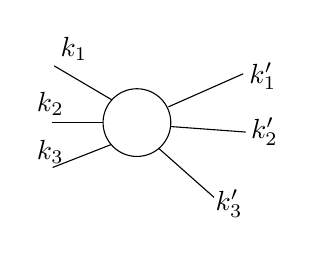
\begin{tikzpicture}[x=1cm,y=1cm]
\draw (0,0) circle (0.43);
\draw (-1.05,0.72) -- (-0.32,0.29);
\draw (-1.08,0) -- (-0.43,0);
\draw (-1.07,-0.57) -- (-0.33,-0.28);
\draw (0.40,0.20) -- (1.35,0.62);
\draw (0.43,-0.05) -- (1.38,-0.12);
\draw (0.28,-0.33) -- (0.98,-0.95);
\node at (-0.80,0.94) {$k_1$};
\node at (-1.10,0.24) {$k_2$};
\node at (-1.10,-0.37) {$k_3$};
\node at (1.60,0.59) {$k_1'$};
\node at (1.62,-0.11) {$k_2'$};
\node at (1.17,-1.03) {$k_3'$};
\end{tikzpicture}
\end{adjustbox}
\end{center}

[Справа от рисунка:] \underline{Зак. сохр. имп. и энергии}
всё опр. лишь для двух.

\underline{Интегрируемость:} есть ещё ряд законов сохр.

Усл. сшивки — ум. на матрицу!

Есть аналогичный анзац Бете для любой интегр. системы.

Неинтегрируемый случай: $O(N)$ даже с $\delta$-обр. потенциалом.

\SourcePage{GELFAND-P001154}{unlabelled}
% Review coordinates: original pixels, upper-left origin;
% rectangles are (x0,y0,x1,y1). Enlargements add no source pixels.
% 1154-heading: original pixel box (130,175,2260,425); 3x.
% 1154-top-math: original pixel box (50,420,2200,1040); 3x.
% 1154-laplace: original pixel box (45,1040,1535,1790); 3x.
% 1154-mass: original pixel box (220,1785,2290,2070); 3x.
% 1154-block: original pixel box (60,2080,1950,2520); 3x.
% 1154-vigman: original pixel box (65,2520,2290,2970); 3x.
% 1154-bottom: original pixel box (180,2945,2290,3445); 3x.
% 1154-radius: original pixel box (820,865,980,1015); 8x.
% 1154-mass-deletion: original pixel box (1570,1770,1820,1930); 6x.
% 1154-doodle: original pixel box (2210,1870,2310,1990); 8x.
% 1154-heading-part: original pixel box (185,2515,495,2640); 5x.
% 1154-coupling: original pixel box (970,2760,1115,2930); 8x.
% 1154-kinetic-sign: original pixel box (690,2760,865,2920); 8x.
% 1154-title-end: original pixel box (1870,2580,2265,2790); 4x.
% 1154-complex: original pixel box (1060,3230,1450,3340); 5x.
% 1154-title-peer-review: original page P001154; crop (x0,y0,x1,y1)=(1270, 2580, 1740, 2720); displayed at 6x.
% Original frame: 2432 x 3480 pixels. A new visible date and two speakers occur
% within this frame; no boundary was supplied from the catalogue.
\underline{12/XII-83 г.}\qquad Сем. Гельфанда

\underline{\underline{В. Гинзбург.}}

\underline{Об одной раб. Witten'a, содержащей попытку}
\newline
\underline{объединить гравитацию и эл.-магн. поле.}

I. $M=\mathbb{R}^4\times S^1$, и $S^1$ — маленькая окружность.

\begin{equation}
R_{ij}-\frac{1}{2}g_{ij}R=0
\qquad\text{(ур-е Эйнштейна)}
\tag{1}
\end{equation}
(пишем его на $M$)

$g_{ij}$ — $5\times5$-матрица
\begin{adjustbox}{max width=\linewidth}
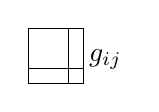
\begin{tikzpicture}[x=1cm,y=1cm,baseline=0.18cm]
\draw (0,0) rectangle (0.70,0.70);
\draw (0.51,0) -- (0.51,0.70);
\draw (0,0.19) -- (0.70,0.19);
\node at (0.98,0.30) {$g_{ij}$};
\end{tikzpicture}
\end{adjustbox}
(блочная).

Разложим $g$ на $S^1$ в ряд Фурье по $\varphi\in S^1$.
\begin{equation}
g=\sum g_k(x)e^{ik\varphi/r}
\tag{2}
\end{equation}
($r$ — радиус маленькой окружности)

Грав. поле мало $\rightsquigarrow$ ур-е Лапласа.

Пишем ур-е Лапласа:
\begin{equation}
0=\left(\Box_4+\frac{\partial^2}{\partial\varphi^2}\right)g
\tag{3}
\end{equation}

отсюда и из (2):
\begin{equation}
\Box_4g_k=\frac{k^2}{r^2}g_k
\tag{4}
\end{equation}

$\Rightarrow$ $k$-е слагаемое — частица с массой
$\Unclear{GELFAND-P001154}{mass-versus-mass-square}{k^2/r^2}$.

$k\ne0$ $\Rightarrow$ при $r\sim$ рад. эл-на получается
$m\sim10^{37}$ [зачёркнуто:
\Unclear{GELFAND-P001154}{mass-cancelled-unit}{неразборчиво}]
эв, чего не бывает
\SourceFigure{GELFAND-P001154}{mass-margin-mark}{Справа после «не бывает»:
маленький наклонный овальный контур над двумя пересекающимися штрихами;
нижний знак похож на $x$ или $\chi$.}

Поэтому $g=g(x)$ (но это тоже не спасает).

% The rectangle and its partitions are drawn conservatively from the manuscript.
% Review box (original pixels): [60,2080,1950,2360], checked at 3x.
\begin{equation}
g_{ij}=
\begin{adjustbox}{max width=\linewidth}
\begin{tikzpicture}[x=1cm,y=1cm,baseline=0.7cm]
\draw (0,0) rectangle (2.15,1.72);
\draw (1.65,0) -- (1.65,1.72);
\draw (0,0.35) -- (2.15,0.35);
\node at (0.84,1.23) {обычн.};
\node at (0.84,0.85) {гравит.};
\draw (2.03,0.35) -- (2.15,0.43);
\draw (1.78,0.35) -- (2.15,0.68);
\draw (1.65,0.48) -- (2.15,0.93);
\draw (1.65,0.73) -- (2.15,1.18);
\draw (1.65,0.98) -- (2.15,1.43);
\draw (1.65,1.23) -- (2.15,1.68);
\draw (1.65,1.48) -- (1.90,1.72);
\draw[<-] (1.93,1.02) -- (2.78,1.02);
\node[align=left,anchor=west] at (2.83,1.02)
{4-мерн. вектор =\\потенц. эл.-магн. поля};
\end{tikzpicture}
\end{adjustbox}
\tag{5}
\end{equation}

(теор. Калуцы — Клейна)

Заряд тоже большой (слишком) получается.

II \Unclear{GELFAND-P001154}{second-part-abbreviation}{час.}
Положительность энергии гравитационного поля.

\underline{\underline{П. Вигман.}}\qquad (продолжение).

\underline{Квант. интегрир. системы на примере или}
\newline
\underline{Об одномерном ферми-газе с $\delta$-обр. притяжением.}
% A yellow digital comment icon is visible at original pixels
% [2140,2590,2270,2725]. No comment text is visible. The handwritten title
% remains readable and no content is inferred from the icon.

\begin{equation}
\mathcal{H}=-\sum_\sigma\psi_\sigma^+(x)
\frac{d^2}{dx^2}\psi_\sigma+
c\left(\sum_\sigma\psi_\sigma^+\psi_\sigma\right)
\left(\sum_{\sigma'}\psi_{\sigma'}^+\psi_{\sigma'}\right)
\tag{1}
\end{equation}
$\sigma=\pm1$.

Классич. аналог — НУШ (нелин. ур-е Шред.), вполне интегр.
(Зах.-Шабат).

Квант. задача решена на 40 лет раньше Бете.

C. N. Yang решил эту задачу.

\begin{equation*}
\psi_\sigma=
\begin{pmatrix}\psi_+\\\psi_-\end{pmatrix}
=
\begin{pmatrix}\psi_\uparrow\\\psi_\downarrow\end{pmatrix}
\qquad\text{Компл. поле — есть ещё }\psi^+.
\end{equation*}

\SourcePage{GELFAND-P001155}{42}
% Review coordinates: original pixels, upper-left origin;
% rectangles are (x0,y0,x1,y1). Enlargements add no source pixels.
% 1155-top-a: GELFAND-P001155; (135, 35, 1250, 685); 3x
% 1155-top-b: GELFAND-P001155; (1265, 35, 2380, 660); 3x
% 1155-mid: GELFAND-P001155; (255, 1300, 2190, 1725); 3x
% 1155-formula10: GELFAND-P001155; (330, 2500, 2200, 2770); 4x
% 1155-bottom: GELFAND-P001155; (280, 2890, 2350, 3420); 3x
% 1155-small-eq2: GELFAND-P001155; (1670, 35, 1930, 200); 10x
% 1155-cancel: GELFAND-P001155; (1680, 1540, 2040, 1678); 8x
% 1155-cancel52: GELFAND-P001155; (320, 1350, 575, 1475); 6x
% 1155-eq3-6: GELFAND-P001155; (130, 800, 2100, 1360); 3x
% 1155-young: GELFAND-P001155; (500, 1660, 930, 1940); 5x
% 1155-eq8-9: GELFAND-P001155; (135, 2025, 2220, 2490); 3x
% 1155-insertion: original bbox (1735, 1555, 2165, 1675); enlargement 6x.

\begin{equation}
\begin{aligned}
\{\psi^+(x),\psi(y)\}&=\delta(x-y)\qquad\text{(фермионы)}\\
\{\psi_\sigma^+\text{\Unclear{GELFAND-P001155}{eq2-argument}{(x)?}},\psi_{\sigma'}(y)\}&=\delta(x-y)\delta_{\sigma\sigma'}
\end{aligned}
\tag{2}
\end{equation}

$\psi^+$ — опер. рождения, $\psi$ — опер. уничтожения

\underline{оглавление.}

\begin{enumerate}
\item Подстановка Бете и законы сохр.
\item Условия интегрируемости (ур-я треугольника)
\item Диагонализация трансфер-матрицы (громоздкие вычисления)

— наиболее простой способ — Фаддеев и др.
\end{enumerate}

Надо решить ур-е Шредингера:
\begin{equation}
\mathcal H|\phi\rangle=E|\phi\rangle
\tag{3}
\end{equation}
\begin{equation}
N=\int dx\sum_\sigma\psi_\sigma^+(x)\psi_\sigma(x)
\qquad\text{(оператор числа частиц)}
\tag{4}
\end{equation}
\begin{equation}
[N,\mathcal H]=0,\quad[\mathcal H,S]=0,\quad\text{где}
\tag{5}
\end{equation}
\begin{equation}
\text{$S$ — \underline{опер. спина}:}\qquad
S=\int dx\sum_\sigma\sigma\psi_\sigma^+(x)\psi_\sigma(x)
\tag{6}
\end{equation}

[Зачёркнуто: \Unclear{GELFAND-P001155}{cancelled-reference}{неразборчивый знак}.]
$(5_2)$ — сохр. спина (у $SU(2)$-симметрии)

Будем искать $|\phi\rangle$ с фиксир. числом частиц и спином.

Предст. группы подст. будем классиф. с пом.
[зачёркнуто: \Unclear{GELFAND-P001155}{young-cancellation}{неразборчивое слово}; над зачёркнутым словом вписано: «(диаграммы)»] Юнга

\begin{center}
(7)\quad
\begin{adjustbox}{max width=\linewidth}
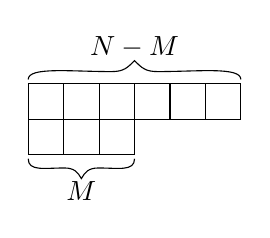
\begin{tikzpicture}[x=0.45cm,y=0.45cm,baseline=(current bounding box.center)]
\draw (0,1) rectangle (6,2);
\draw (0,0) rectangle (3,1);
\draw (1,0)--(1,2);
\draw (2,0)--(2,2);
\draw (3,1)--(3,2);
\draw (4,1)--(4,2);
\draw (5,1)--(5,2);
\draw (0,2.12) .. controls (0,2.48) and (1.2,2.34) .. (2.35,2.34)
 .. controls (2.7,2.34) and (2.8,2.45) .. (3,2.65)
 .. controls (3.2,2.45) and (3.3,2.34) .. (3.65,2.34)
 .. controls (4.8,2.34) and (6,2.48) .. (6,2.12);
\node at (3,3.02) {$N-M$};
\draw (0,-0.12) .. controls (0,-0.48) and (0.45,-0.38) .. (1.02,-0.38)
 .. controls (1.3,-0.38) and (1.4,-0.5) .. (1.5,-0.68)
 .. controls (1.6,-0.5) and (1.7,-0.38) .. (1.98,-0.38)
 .. controls (2.55,-0.38) and (3,-0.48) .. (3,-0.12);
\node at (1.5,-1.03) {$M$};
\end{tikzpicture}
\end{adjustbox}
\end{center}

Здесь полный спин
\begin{equation}
S=N-M-M=N-2M
\tag{8}
\end{equation}
($M$ — число частиц со знаком \Unclear{GELFAND-P001155}{spin-sign-convention}{$\uparrow$}, остальные $\downarrow$)

(9) [Слева две вертикальные черты.]
Волн. ф-я симметр. по частицам, соотв. верхней строке и антисимм. по част. \Unclear{GELFAND-P001155}{lower-row-antisymmetry}{нижней строки}.

\begin{equation}
\begin{aligned}
|\phi\rangle={}&\int
\text{\ReaderApparatusRef{1}{1}}
\psi_{\sigma_1}^+(x_1)\ldots\psi_{\sigma_N}^+(x_N)\\
&\qquad dx_1\ldots dx_N\,|0\rangle
\end{aligned}
\tag{10}
\end{equation}

\begin{equation}
|0\rangle\text{ — вакуум};\qquad\psi|0\rangle=0
\tag{11}
\end{equation}

(12) $\phi_{\sigma_1\ldots\sigma_N}(x_1,\ldots,x_N)$ \underline{наз. волновой функцией}.

[На правом поле, отделено двумя вертикальными чертами:]
антисимм. при перем. $(x_i,\sigma_i)$ с $(x_j,\sigma_j)$

Она должна принадл. предст. (7) симметр. группы.

Запись (1) — предст. вторичного квантования.

Первичное — ур-е на $\phi_{\sigma_1\ldots\sigma_N}(x_1,\ldots,x_N)$


\ReaderNotesStart{GELFAND-P001155}
\ReaderNote{1}{\Unclear{GELFAND-P001155}{eq10-spin-summation}{$\phi_{\sigma_1\ldots\sigma_N}(x_1,\ldots,x_N)$}}
\ReaderNotesEnd
\SourcePage{GELFAND-P001156}{unlabelled}
% Review coordinates: original pixels, upper-left origin;
% rectangles are (x0,y0,x1,y1). Enlargements add no source pixels.
% 1156-top: GELFAND-P001156; (80, 35, 2350, 380); 3x
% 1156-eq14: GELFAND-P001156; (65, 410, 1550, 650); 4x
% 1156-middle: GELFAND-P001156; (240, 1170, 2240, 1940); 3x
% 1156-formula16: GELFAND-P001156; (270, 2250, 1570, 2550); 5x
% 1156-scatter: GELFAND-P001156; (430, 2910, 1310, 3420); 4x
% 1156-uppertext: GELFAND-P001156; (210, 675, 2260, 1275); 3x
% 1156-antisym-line: GELFAND-P001156; (715, 1560, 2350, 1780); 4x
% 1156-eq15: GELFAND-P001156; (200, 1900, 2340, 2240); 3x
% 1156-subp: GELFAND-P001156; (1340, 2320, 1470, 2450); 10x
% 1156-heading: original pixel bbox (270, 2770, 1970, 2950); enlargement 3x.
% 1156-headingword: original bbox (215, 2820, 705, 2945); enlargement 6x.
% 1156-biblio: original bbox (960, 1835, 1795, 1935); enlargement 4x.
% 1156-biblioending: original bbox (1470, 1840, 1650, 1925); enlargement 8x.
% 1156-na-phi: original bbox (410, 300, 490, 385); enlargement 10x.

(13) \SourceFigure{GELFAND-P001156}{young-pair}{Слева две горизонтальные строки, верхняя длиннее нижней; у левого конца разделяющей их линии имеется короткий штрих, похожий на наконечник влево. Справа две вертикальные колонки, левая длиннее правой, с общей верхней границей. Неясно, является ли короткий штрих слева стрелкой.}

[Подпись к левой фигуре:] д. Юнга коорд.

[Подпись к правой фигуре:] д. Юнга для спинов

(ширина 2 т.к. 2 знач. спина $\pm1$)

На $\phi$ получ.:
\begin{equation}
\left\{-\sum_{i=1}^N\frac{\partial^2}{\partial x_i^2}
+c\sum_{i>j}\delta(x_i-x_j)\right\}\Phi=E\Phi
\tag{14}
\end{equation}
[Последняя цифра номера (14) исправлена: \Unclear{GELFAND-P001156}{eq14-number-correction}{прежняя цифра неразборчива}.]

\underline{Пояснение:}

$\Phi_{\sigma_1\ldots\sigma_N}(x_1,\ldots,x_N)$ — антисимм. при перест. пар $(x_i,\sigma_i),(x_j,\sigma_j)$.

Что при перест. только коорд. при зад. наборе $\sigma_i$?
\begin{equation*}
\phi=\sum f(x_1,\ldots,x_N)\chi(\sigma_1,\ldots,\sigma_N)
\end{equation*}
(сумма тензоров; всегда так можно сделать; тогда вводим только пары $f,\chi$ с опр. симметриями)
\begin{equation*}
\Phi(x,\sigma)=\sum_{\tau_1,\tau_2}f_{\tau_1}(x)g_{\tau_2}(\sigma)
\end{equation*}
$\tau_1,\tau_2$ — предст. симм. группы.

$\Phi$ антисимм. $\Rightarrow$ прис. лишь \Unclear{GELFAND-P001156}{antisymmetry-abbreviation}{слн. / слм. / слаг.?}, соотв. представлениям, дополн. друг друга

\begin{center}
\begin{adjustbox}{max width=\linewidth}
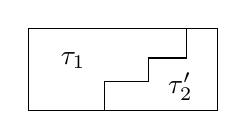
\begin{tikzpicture}[x=0.6cm,y=0.6cm]
\draw (0,0) rectangle (4,1.75);
\draw (3.35,1.75)--(3.35,1.12)--(2.55,1.12)--(2.55,0.63)--(1.62,0.63)--(1.62,0);
\node at (0.95,1.07) {$\tau_1$};
\node at (3.22,0.52) {$\tau_2'$};
\end{tikzpicture}
\end{adjustbox}
\end{center}

(см. § в главе «Спин» \underline{кн.} Ландау и Лифшица, т. 3)

Рассм. область
\begin{equation}
X_Q=\{x_{q_1}<\ldots<x_{q_N}\}
\qquad\text{($Q$ — перестановка $(1,2,\ldots,N)$)}
\tag{15}
\end{equation}
Ответ в $X_Q$ — подстановка Бете:
\begin{equation}
\Phi=\sum A_{\sigma_{q_1}\ldots\sigma_{q_N}}(Q\cdot P)(-1)^P
\exp i\sum_{j=1}^N k_{\text{\ReaderApparatusRef{1}{1}}}x_j
\tag{16}
\end{equation}

$(k_1,\ldots,k_N)$ — импульсы, задающие волн. функцию.
\begin{equation*}
E=\sum_j k_j^2.
\end{equation*}

\Unclear{GELFAND-P001156}{heading-formula16}{Непривычность / Непрерывность?} формулы (16):

\begin{center}
(17)\quad
\begin{adjustbox}{max width=\linewidth}
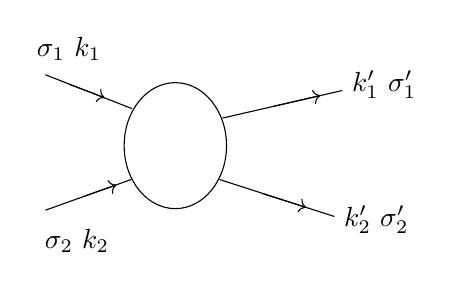
\begin{tikzpicture}[x=1cm,y=1cm,baseline=(current bounding box.center)]
\draw (0,0) ellipse (0.65 and 0.8);
\draw (-1.65,0.9)--(-0.55,0.47);
\draw[->] (-1.35,0.78)--(-0.9,0.61);
\draw (-1.65,-0.82)--(-0.56,-0.43);
\draw[->] (-1.15,-0.64)--(-0.75,-0.50);
\draw (0.6,0.35)--(2.12,0.7);
\draw[->] (1.25,0.50)--(1.84,0.635);
\draw (0.56,-0.43)--(2.02,-0.9);
\draw[->] (1.11,-0.61)--(1.66,-0.785);
\node[above] at (-1.35,0.96) {$\sigma_1\ k_1$};
\node[below] at (-1.25,-0.94) {$\sigma_2\ k_2$};
\node[right] at (2.12,0.77) {$k_1'\ \sigma_1'$};
\node[right] at (2.02,-0.94) {$k_2'\ \sigma_2'$};
\end{tikzpicture}
\end{adjustbox}

\underline{Рассеяние}
\end{center}


\ReaderNotesStart{GELFAND-P001156}
\ReaderNote{1}{\Unclear{GELFAND-P001156}{eq16-momentum-index}{$P_j$ / $p_j$?}}
\ReaderNotesEnd
\SourcePage{GELFAND-P001157}{43}
% Review coordinates: original pixels, upper-left origin;
% rectangles are (x0,y0,x1,y1). Enlargements add no source pixels.
% 1157-top: GELFAND-P001157; (250, 35, 2340, 880); 3x
% 1157-middle: GELFAND-P001157; (250, 1380, 2380, 1920); 3x
% 1157-eq23-25: GELFAND-P001157; (320, 1910, 1700, 2640); 3x
% 1157-bottom: GELFAND-P001157; (350, 2720, 2350, 3410); 3x
% 1157-abbrev: original pixel bbox (1020, 480, 1510, 580); enlargement 6x.
% 1157-permutationword: original pixel bbox (1790, 585, 2140, 705); enlargement 6x.
% 1157-eq25-indices: original pixel bbox (470, 2440, 625, 2530); enlargement 10x.
% 1157-eq20-indices: original pixel bbox (410, 532, 537, 593); enlargement 10x.
% 1157-3scatter: original pixel bbox (315, 945, 1035, 1345); enlargement 4x.
% 1157-correctedword: original pixel bbox (1310, 3000, 1760, 3110); enlargement 6x.

\begin{equation}
\begin{aligned}
k_1+k_2&=k_1'+k_2'&\quad&\text{(сохр. имп.)}\\
k_1^2+k_2^2&=k_1'^2+k_2'^2&&\text{(сохр. энергии)}
\end{aligned}
\tag{18}
\end{equation}

(19) Этого достаточно (в 1-мер. случае) для фиксации $(k_1,k_2)$ (с точн. до перестановки).
\underline{Может произойти лишь смена спина.}

$S$-матрица (потом будет \Unclear{GELFAND-P001157}{s-matrix-abbreviation}{сущ. / сл.?} следующее)
\begin{equation}
S_{\sigma_1\sigma_2}^{\sigma_1'\sigma_2'}(k_1,k_2)=bI+cP
\qquad\text{($P$ — опер. перестройки)}
\tag{20}
\end{equation}

$(\sigma_1,\sigma_2)$ — нач. спины, $(\sigma_1',\sigma_2')$ — конечные

Рассм. 3-част. рассеяние:

\SourceFigure{GELFAND-P001157}{three-particle-scattering}{Овал с тремя отрезками слева и тремя справа. Слева сверху вниз подписи $k_1,k_2,k_3$; справа сверху вниз $k_1',k_2',k_3'$. Левые верхний и нижний отрезки наклонены к овалу, средний почти горизонтален; справа верхний идёт вверх, средний горизонтально, нижний вниз. У внешнего конца левого верхнего отрезка короткий угловой штрих: его роль как возможного наконечника неясна.}

\begin{equation}
\sum k_j=\mathrm{const},\qquad\sum k_j^2=\mathrm{const}
\qquad\text{— недостаточно}
\tag{21}
\end{equation}

Но: из-за интегрируемости здесь
\begin{equation}
\sum k_j^n=\mathrm{const},\qquad n=1,2,3,\ldots
\tag{22}
\end{equation}

(отсутствие множественного рождения; единств. событие — перемешивание спинов частиц)

\begin{equation}
\begin{array}{cc}
\sigma_1&k_1\\
\vdots&\vdots\\
\sigma_n&k_n
\end{array}
\longmapsto
\begin{array}{cc}
\sigma_{q_1}&k_1\\
\vdots&\vdots\\
\sigma_{q_n}&k_n
\end{array}
\tag{23}
\end{equation}

\underline{Опр. матрицы рассеяния:}
\begin{equation}
A(Q)=\widehat S A(Q')
\tag{24}
\end{equation}

Пусть 2 меняются местами:
\begin{equation}
S_{\sigma_1\sigma_2}^{\sigma_1'\sigma_2'}(k_1,k_2)=
\begin{adjustbox}{max width=\linewidth}
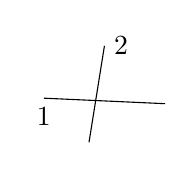
\begin{tikzpicture}[x=0.7cm,y=0.7cm,baseline=(current bounding box.center)]
\draw (0,0)--(2.2,-0.1);
\draw (0.82,-0.8)--(1.1,0.95);
\node[below] at (0,0) {$1$};
\node[right] at (1.1,0.95) {$2$};
\end{tikzpicture}
\end{adjustbox}
\qquad\text{(обозначение)}
\tag{25}
\end{equation}

$n$-частичная:
\begin{equation}
S_{\sigma_1\ldots\sigma_n}^{\sigma_1'\ldots\sigma_n'}(k_1,\ldots,k_n)=
\begin{adjustbox}{max width=\linewidth}
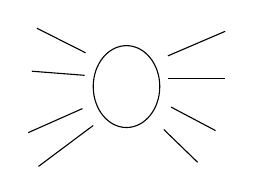
\begin{tikzpicture}[x=0.65cm,y=0.65cm,baseline=(current bounding box.center)]
\draw (0,0) ellipse (0.65 and 0.8);
\draw (-1.75,1.14)--(-0.8,0.66);
\draw (-1.85,0.3)--(-0.82,0.22);
\draw (-1.92,-0.9)--(-0.86,-0.43);
\draw (-1.72,-1.56)--(-0.65,-0.76);
\draw (0.81,0.6)--(1.93,1.08);
\draw (0.82,0.15)--(1.92,0.15);
\draw (0.87,-0.40)--(1.74,-0.86);
\draw (0.73,-0.84)--(1.39,-1.48);
\end{tikzpicture}
\end{adjustbox}
\tag{26}
\end{equation}

(27) \underline{Утв.:} (26) = произведение 2-частичных
[в слове «2-частичных» исправлены буквы: \Unclear{GELFAND-P001157}{eq27-corrected-letters}{прежние буквы неразборчивы}] матриц рассеяния.

\begin{equation}
\begin{adjustbox}{max width=\linewidth}
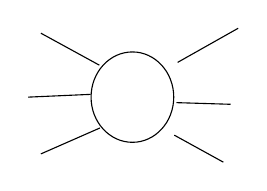
\begin{tikzpicture}[x=0.7cm,y=0.7cm,baseline=(current bounding box.center)]
\draw (0,0) ellipse (0.75 and 0.82);
\draw (-1.66,1.16)--(-0.60,0.58);
\draw (-1.89,0)--(-0.76,0.05);
\draw (-1.66,-1.03)--(-0.59,-0.56);
\draw (0.82,0.63)--(1.92,1.25);
\draw (0.80,-0.1)--(1.78,-0.13);
\draw (0.76,-0.69)--(1.65,-1.18);
\end{tikzpicture}
\end{adjustbox}
\quad=\quad
\begin{adjustbox}{max width=\linewidth}
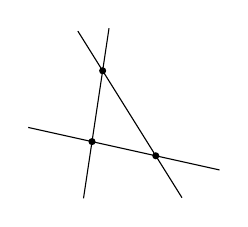
\begin{tikzpicture}[x=0.9cm,y=0.9cm,baseline=(current bounding box.center)]
\draw (0.83,-1.0)--(1.19,1.4);
\draw (0.75,1.36)--(2.22,-0.992);
\draw (0.05,0)--(2.75,-0.6);
\fill (1.1,0.8) circle (0.05);
\fill (0.95,-0.2) circle (0.05);
\fill (1.85,-0.4) circle (0.05);
\end{tikzpicture}
\end{adjustbox}
\tag{28}
\end{equation}

\SourcePage{GELFAND-P001158}{unlabelled}
% Review coordinates: original pixels, upper-left origin;
% rectangles are (x0,y0,x1,y1). Enlargements add no source pixels.
% 1158-phase: source GELFAND-P001158.png; original bbox (1110, 2615, 1230, 2725); enlargement 10x.
% 1158-automatic: source GELFAND-P001158.png; original bbox (1470, 2650, 2240, 2760); enlargement 3x.
% 1158-eq31-middle: source GELFAND-P001158.png; original bbox (1010, 1490, 1160, 1610); enlargement 8x.
% 1158-eq32-lowerline: source GELFAND-P001158.png; original bbox (610, 1935, 720, 2085); enlargement 8x.
% 1158-bottomparenthesis: source GELFAND-P001158.png; original bbox (1210, 3110, 1585, 3235); enlargement 5x.
% 1158-diag29: original pixel crop (75, 0, 740, 390), enlargement 3x
% 1158-eq30: original pixel crop (250, 400, 1750, 675), enlargement 3x
% 1158-text1: original pixel crop (265, 690, 2280, 1300), enlargement 2x
% 1158-mid: original pixel crop (65, 1330, 2200, 2100), enlargement 2x
% 1158-text2: original pixel crop (230, 2080, 2300, 2460), enlargement 2x
% 1158-bottom: original pixel crop (230, 2650, 2320, 3330), enlargement 2x
% 1158-eq30-indices: original pixel crop (1160, 410, 1725, 615), enlargement 6x
% 1158-first-text: original pixel crop (280, 700, 1300, 1080), enlargement 3x
% 1158-first-text-right: original pixel crop (1200, 690, 2250, 870), enlargement 3x
% 1158-conditions: original pixel crop (270, 1090, 1600, 1300), enlargement 3x
% 1158-insertion: original pixel crop (300, 800, 520, 891), enlargement 6x
% 1158-hardballs: original pixel crop (270, 995, 1650, 1100), enlargement 3x
% 1158-collision-note: original pixel crop (1580, 1460, 2070, 1590), enlargement 3x
% 1158-finaltext: original pixel crop (295, 3000, 2310, 3300), enlargement 3x
% 1158-eq34-rhs: original pixel crop (1420, 2870, 2335, 3030), enlargement 5x
% 1158-diag33: original pixel crop (540, 2440, 1180, 2660), enlargement 4x
% 1158-last-parenthesis: original pixel crop (1235, 3110, 1570, 3225), enlargement 6x
% 1158-diag32-left: original pixel crop (332, 1632, 730, 2100), enlargement 4x
% 1158-diag32-arrow: original pixel crop (610, 1950, 725, 2085), enlargement 9x
% 1158-phase: original pixel crop (1085, 2648, 1210, 2745), enlargement 8x
% 1158-diag31-middle-label: GELFAND-P001158; original box=(1010, 1480, 1170, 1638); enlargement=8x; direct crop for final recheck.
% 1158-netriv-comparison: GELFAND-P001158; original box=(1010, 2750, 1390, 2860); enlargement=5x; direct crop for final recheck.
% 1158-netriv-word: GELFAND-P001158; original box=(735, 2750, 1010, 2860); enlargement=5x; final literal peer recheck.
% 1158-automatic: GELFAND-P001158; original box=(1470, 2650, 2240, 2760); enlargement=3x; final literal peer recheck.
(29)
\begin{center}
\begin{adjustbox}{max width=\linewidth}
\begin{tikzpicture}[x=1cm,y=1cm]
\draw (0,0.65) -- (2.75,3.05);
\draw (0.95,3.05) -- (2.8,0.45);
\draw (-0.25,1.55) .. controls (0.4,1.35) and (2.6,1.35) .. (3.8,1.3);
\node at (-0.05,0.12) {$\sigma_1$};
\node at (3.25,3.2) {$\sigma_1'$};
\node at (0.48,3.15) {$\sigma_3$};
\node at (3.2,0.12) {$\sigma_3'$};
\node at (-0.65,1.45) {$\sigma_2$};
\node at (4.25,1.25) {$\sigma_2'$};
\node at (1.05,1.95) {$\tau_1$};
\node at (1.58,1.02) {$\tau_2$};
\end{tikzpicture}
\end{adjustbox}
\end{center}
\begin{equation*}
S_{\sigma_1\sigma_2\sigma_3}^{\sigma_1'\sigma_2'\sigma_3'}(k_1,k_2,k_3)
=\sum_{\tau}
S_{\tau_2\tau_3}^{\sigma_2'\sigma_3'}(k_2,k_3)
S_{\Unclear{GELFAND-P001158}{eq30-middle-lower-index}{\tau_2\sigma_3}}^{\sigma_1'\tau_3}(k_1,k_3)
S_{\sigma_1\sigma_2}^{\tau_1\tau_2}(k_1,k_2)
\tag{30}
\end{equation*}

Не каждый объект так предст. (через 2-частичные акты рассеяния)
[Под строкой, обведено и присоединено к слову «объект»: (или $S$).]

Но в интегр. системах это так!!

Всё как в сист. сталкив. твёрдых шариков и т. д.

\underline{Условие сущ. предст. (30)} — уравнение $\triangle$-ка

(необх. и дост.)

(31)
\begin{center}
\begin{adjustbox}{max width=\linewidth}
\begin{tikzcd}
x_1<x_2<x_3 \arrow[rr,mapsto] \arrow[dr,"S_{23}"'] && x_3<x_2<x_1 \\
& x_1<x_3<x_2 \arrow[r,"S_{13}"] & x_3<x_1<x_2 \arrow[u,"S_{12}"']
\end{tikzcd}
\end{adjustbox}
\end{center}
(через попарные)

(32)
\SourceFigure{GELFAND-P001158}{diagram32}{Два рисунка по три пересекающиеся линии. Слева линия $1$ почти вертикальна, линия $2$ спускается вправо, линия $3$ идёт слева направо с небольшим наклоном вниз; подпись $1$ стоит у верхнего конца вертикальной линии, $2$ у верхнего конца нисходящей, $3$ слева. У верхнего конца линии $1$ короткий боковой штрих, а ниже пересечения $1$ и $2$ линия $2$ утолщена; неясно, обозначают ли эти детали стрелки. Рядом с левым рисунком отдельная стрелка направлена вверх-вправо. Справа линии $1$ и $2$ пересекаются выше почти горизонтальной линии $3$; $1$ поднимается вправо, $2$ спускается вправо, на её нижнем конце видна стрелка. Подписи $1$ и $2$ стоят сверху, $3$ слева. Большая изогнутая стрелка от текста «Есть другой процесс:» направлена вверх-вправо к правому рисунку.}

Есть другой процесс:

тогда

$S_{12}\ S_{13}\ S_{23}$ — порядок столкновений

(33) \underline{Условие}: результат рассеяния должен быть тот же при всех
способах: символич. это пишется так
\begin{center}
\begin{adjustbox}{max width=\linewidth}
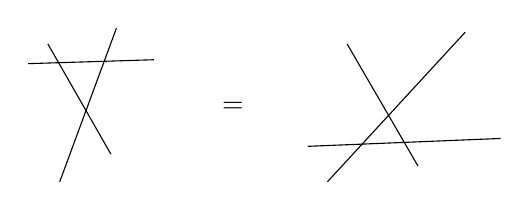
\begin{tikzpicture}[x=1cm,y=1cm]
\draw (0.25,1.75) -- (1.05,0.35);
\draw (0.4,0) -- (1.12,1.95);
\draw (0,1.5) -- (1.6,1.55);
\node at (2.6,0.95) {$=$};
\draw (4.05,1.75) -- (4.95,0.2);
\draw (3.8,0) -- (5.55,1.9);
\draw (3.55,0.45) -- (6,0.55);
\end{tikzpicture}
\end{adjustbox}
\end{center}
Без изотопич. индексов: $S=e^{i\Unclear{GELFAND-P001158}{phase-symbol}{\varphi}}$ и всё автоматич. выполняется.

С индексами — нетрив. соотношение:
\begin{equation*}
S_{23}(k_2,k_3)S_{13}(k_1,k_3)S_{12}(k_1,k_2)
=S_{12}(k_1,k_2)\Unclear{GELFAND-P001158}{eq34-rhs-middle}{S_{23}(k_1,k_3)}S_{23}(k_2,k_3)
\tag{34}
\end{equation*}

Это необх. и дост. условие интегрируемости квант. систем. Так
описываются все квант. интегр. сист.

Интересно, что они существуют!! (\Unclear{GELFAND-P001158}{bottom-parenthesis}{нетрив. [?]})

До конца не классифицированы.

\SourcePage{GELFAND-P001159}{44}
% Review coordinates: original pixels, upper-left origin;
% rectangles are (x0,y0,x1,y1). Enlargements add no source pixels.
% 1159-eq36-abbrev: source GELFAND-P001159.png; original bbox (1260, 520, 1530, 635); enlargement 5x.
% 1159-tetraedra: source GELFAND-P001159.png; original bbox (530, 795, 785, 905); enlargement 5x.
% 1159-eq38-first: source GELFAND-P001159.png; original bbox (520, 1810, 845, 1960); enlargement 6x.
% 1159-top: original pixel crop (250, 0, 1220, 170), enlargement 3x
% 1159-eq35: original pixel crop (250, 160, 2370, 475), enlargement 3x
% 1159-eq36: original pixel crop (245, 515, 2220, 723), enlargement 3x
% 1159-tetrahedron: original pixel crop (240, 720, 2380, 890), enlargement 3x
% 1159-textmiddle: original pixel crop (260, 880, 2280, 1370), enlargement 3x
% 1159-crossedhead: original pixel crop (285, 1380, 2375, 1560), enlargement 4x
% 1159-eq37: original pixel crop (350, 1510, 2240, 1820), enlargement 3x
% 1159-eq38: original pixel crop (360, 1835, 2230, 1995), enlargement 4x
% 1159-bottom: original pixel crop (280, 2030, 2325, 3370), enlargement 2x
% 1159-tetra-line: original pixel crop (285, 814, 1125, 895), enlargement 5x
% 1159-yang: original pixel crop (670, 8, 830, 100), enlargement 7x
% 1159-head-crossout: original pixel crop (290, 1387, 1005, 1515), enlargement 6x
% 1159-coefficient: original pixel crop (767, 1540, 1110, 1660), enlargement 8x
% 1159-diagram: original pixel crop (735, 1663, 1115, 1830), enlargement 6x
% 1159-cancelled-note: original pixel crop (1735, 1795, 2190, 1908), enlargement 6x
% 1159-eq39indices: original pixel crop (725, 2225, 933, 2420), enlargement 6x
% 1159-multiple-scattering: original pixel crop (975, 1280, 1825, 1380), enlargement 4x
% 1159-cancelled-note-low: original pixel crop (1725, 1780, 2220, 1915), enlargement 3x
% 1159-final-dimension: original pixel crop (287, 1092, 893, 1200), enlargement 4x
% 1159-urya: GELFAND-P001159; original box=(1260, 520, 1530, 635); enlargement=5x; final literal peer recheck.
1-е реш. нашёл Янг.

$2\times2$ все реш. нашёл Бакстер

(35) \underline{Утв.} $\exists$ параметризация $k(\theta)$, такая что
$S(k,k')=S(\theta-\theta')$

\begin{equation*}
\left(\begin{array}{ll}
\underline{\text{соотв.}}&k=m\,\mathrm{sh}\,\theta\\
&\varepsilon=m\,\mathrm{ch}\,\theta
\end{array}\right)
\end{equation*}

[Справа, отделено двумя наклонными чертами:]
$\theta-\theta'$ соотв. гр. Галилея
и гр. Лоренца

(36) \underline{Белавин, Дринфельд} изуч. квазиклассич. ур-я $\triangle$-ка:
$S=1+\hbar r$

(решали соотв. квадр. ур-е)

\underline{Тетраэдр:} в многомерных зад. надо изучать струны, поверхности и т. д.

Тетраэдры посланы друг к другу

Пока нетрив. решений не найдено (и есть подозрение, что нетрив.
решений нет; если бы были, то получились бы интегр. системы в
высокой размерности)

Реш., найденные Замолодчиковым, описывают своб. частицу.

Их сущ. привело бы к множеств. рассеянию (нетрив.)

\underline{Решение:}
\Unclear{GELFAND-P001159}{heading-cancelled-formula}{[Зачёркнуто: $S(k_1,k_2)$ (?)]}
\underline{ур-й (34) для $2\times2$-матриц с усл. $SU(2)$-инв.}\newline
\underline{по верхн. и нижней парам индексов}

\Unclear{GELFAND-P001159}{heading-cancelled-note}{[Под словом «Решение» зачёркнуто: «ур-я (34)» (?)]}

\begin{equation*}
S_{\sigma_1\sigma_2}^{\sigma_1'\sigma_2'}(k)=I\cdot k+
\Unclear{GELFAND-P001159}{eq37-cancelled-coefficient}{\text{[зачёркнутый коэффициент]}}\hat P,
\qquad \hat P\text{ — опер. перестановки}
\tag{37}
\end{equation*}
\SourceFigure{GELFAND-P001159}{eq37-diagram}{Под формулой слева две дуги: верхняя вогнута вверх, с подписями $\sigma_1$ слева и $\sigma_1'$ справа; нижняя вогнута вниз, с подписями $\sigma_2$ слева и $\sigma_2'$ справа. Далее знак $+$ и две перекрещивающиеся линии без подписей. В области пересечения восходящая линия имеет изгиб; точное устройство пересечения неясно.}

(здесь $k=k_1-k_2$)

\Unclear{GELFAND-P001159}{cancelled-parenthesis}{[Зачёркнуто: $(\lambda$ — параметр.) (?); первый знак также допускает чтение $k$.]}

\begin{equation*}
I=\delta_{\sigma_1\sigma_1'}\delta_{\sigma_2\sigma_2'},
\qquad
\hat P=\delta_{\sigma_1\sigma_2'}\delta_{\sigma_1'\sigma_2}
\tag{38}
\end{equation*}
Это $SU(2)$-инв. решение ур-й $\triangle$-ка.

Сравним с реш. 2-част. задачи.

\begin{equation*}
\left[-\frac{\partial^2}{\partial x_1^2}
-\frac{\partial^2}{\partial x_2^2}
+V_{\sigma_1\sigma_2}^{\sigma_1'\sigma_2'}\delta(x_1-x_2)\right]\Phi=E\Phi
\tag{39}
\end{equation*}
$V$ — матрица, перев. $\sigma_1\sigma_2$ в $\sigma_1'\sigma_2'$

\begin{equation*}
S=\frac{k+i\hat V\cdot\hat P}{k+i\hat V}
\tag{40}
\end{equation*}
(это из реш. ур-я (39))

(преобр. Кэли потенциала $\hat V$).

\underline{Вопрос:} при каких $\hat V$ будет интегрируемость?

(41) \underline{Решения для $SU(2)$:} $\hat V=I$ или $\hat V=\hat P$

(но после переобозначения совпадают)

Для других групп — другие решения и другие потенциалы.

Поэтому $\hat V=I$ и система

\SourcePage{GELFAND-P001160}{unlabelled}
% Review coordinates: original pixels, upper-left origin;
% rectangles are (x0,y0,x1,y1). Enlargements add no source pixels.
% 1160-phase-first: source GELFAND-P001160.png; original bbox (755, 2770, 920, 2875); enlargement 10x.
% 1160-phase-second: source GELFAND-P001160.png; original bbox (1310, 2780, 1480, 2910); enlargement 10x.
% 1160-eq45-phi-left: source GELFAND-P001160.png; original bbox (375, 1160, 470, 1290); enlargement 8x.
% 1160-eq45-phi-right: source GELFAND-P001160.png; original bbox (1250, 1160, 1350, 1265); enlargement 8x.
% 1160-top42-44: original pixel crop (280, 60, 2080, 819), enlargement 3x
% 1160-realparticles: original pixel crop (300, 836, 2140, 1194), enlargement 3x
% 1160-eq45: original pixel crop (355, 1173, 2215, 1325), enlargement 4x
% 1160-conditions: original pixel crop (277, 1312, 2335, 1467), enlargement 3x
% 1160-eq46diagram: original pixel crop (1280, 1425, 2105, 1619), enlargement 5x
% 1160-eq46left: original pixel crop (475, 1415, 892, 1610), enlargement 5x
% 1160-graphicnote: original pixel crop (1510, 1582, 2365, 1745), enlargement 4x
% 1160-eq47: original pixel crop (385, 1613, 1390, 1809), enlargement 4x
% 1160-note47: original pixel crop (1090, 1740, 2379, 1904), enlargement 4x
% 1160-vector-amplitude: original pixel crop (295, 1835, 2390, 2015), enlargement 3x
% 1160-spectrum: original pixel crop (332, 2010, 1655, 2228), enlargement 3x
% 1160-eq48: original pixel crop (330, 2243, 1595, 2440), enlargement 4x
% 1160-transfertext: original pixel crop (332, 2461, 1960, 2703), enlargement 3x
% 1160-eq49-50: original pixel crop (275, 2690, 2110, 2938), enlargement 3x
% 1160-bottom: original pixel crop (305, 2935, 1955, 3438), enlargement 3x
% 1160-cancelled-particle: original pixel crop (1235, 939, 1320, 1045), enlargement 10x
% 1160-cancelled-transfer: original pixel crop (780, 2494, 897, 2589), enlargement 10x
% 1160-cancelled-vector: original pixel crop (442, 3039, 824, 3192), enlargement 7x
% 1160-cancelled-hat: original pixel crop (639, 3200, 760, 3296), enlargement 10x
% 1160-label50: original pixel crop (106, 2791, 243, 2917), enlargement 7x
% 1160-phi50: original pixel crop (1200, 2814, 1465, 2924), enlargement 6x
% 1160-index49: original pixel crop (1722, 2690, 2080, 2825), enlargement 6x
% 1160-diagram-full: original pixel crop (1300, 1400, 2095, 1620), enlargement 4x
% 1160-phase-first: original pixel crop (774, 2774, 934, 2858), enlargement 8x
% 1160-phase-full: GELFAND-P001160; original box=(750, 2760, 995, 2900); enlargement=7x; direct crop for final recheck.
% 1160-Phi-left: GELFAND-P001160; original box=(375, 1160, 470, 1290); enlargement=8x; final literal peer recheck.
% 1160-phi-right: GELFAND-P001160; original box=(1250, 1160, 1350, 1265); enlargement=8x; final literal peer recheck.
% 1160-top-right-mark: GELFAND-P001160; original box=(2340, 0, 2432, 110); enlargement=8x; small mark at paper edge.
\begin{equation*}
\left[-\frac{\partial^2}{\partial x_1^2}
-\frac{\partial^2}{\partial x_2^2}
+\Unclear{GELFAND-P001160}{eq42-43-coupling}{\delta(x_1-x_2)}\right]
\tag{42}
\end{equation*}
интегрируема. Её 2-частичная $S$-матрица имеет вид
\begin{equation*}
S(k)=\frac{k+ic\hat P}{k+ic}
\tag{43}
\end{equation*}

(44) При $\hat V\ne I,\hat P$ система неинтегрируема!!

[\underline{Вопрос:} какая тогда полная сист. соб. ф-й?].

(43) — $S$-матр. голых частиц.

Нас интерес. \underline{реальные} частицы
\Unclear{GELFAND-P001160}{cancelled-particle-symbol}{[Зачёркнутый неразборчивый знак]}.

Спектр — ?. Рассм. периодические гран. условия (период $2L$)
\begin{equation*}
\left.\Phi(x_1,\ldots,x_i,\ldots,x_N)\right|_{x_i=-L}
=\left.\varphi(x_1,\ldots,x_i,\ldots,x_N)\right|_{x_i=L},
\qquad i=1,\ldots,N
\tag{45}
\end{equation*}
Условия надо сформулир. в терминах $S$-матрицы $\{$ возврат к исх. фазе на
отр. $2L$):
\begin{equation*}
\prod_i\hat S(k-k_i)
\tag{46}
\end{equation*}
\SourceFigure{GELFAND-P001160}{eq46-diagram}{Справа от произведения горизонтальная линия со стрелкой влево пересекает шесть наклонных линий, восходящих вправо. Над первыми двумя стоят $\sigma_1$, $\sigma_2$, над последней $\sigma_N$; снизу соответственно $\sigma_1'$, $\sigma_2'$, $\sigma_N'$. Между верхними подписями видны отдельные точки. В пересечениях толстые точки и петли: второе и последнее выглядят незакрашенными, остальные закрашенными, но точное различие неясно. Справа от рисунка написано $=e^{2ikL}$.}

[Под рисунком, со стрелкой вверх к нему:]
графич. запись опер. $\displaystyle\prod_{j\ne i}\hat S_{ji}(k_j-k_i)$

\begin{equation*}
\Unclear{GELFAND-P001160}{eq47-indices-phase}{e^{ik_jL}A=\prod_{j\ne i}\hat S_{ji}(k_j-k_i)A}
\tag{47}
\end{equation*}

(на самом деле $2^N\times2^N$-матр., начальные амплитуды
перех. в конечные)

[От правой части скобочной пометы стрелка направлена вниз-влево к следующей строке.]

$A$ — коэфф. (векторный) в волн. ф-и Бете, стоящий перед экспо-
нентой.

\underline{Спектр:} квантование импульсов в ящике.

Теперь надо решить зад. на соб. знач. (47)
\begin{equation*}
\prod_{j\ne i}\hat S_{ji}(k_j-k_i)\overset{df}{=}\text{трансфер-матрица}
\tag{48}
\end{equation*}
Она переносит
\Unclear{GELFAND-P001160}{cancelled-transfer-symbol}{[зачёркнуто: $\Phi$ (?)]}
от одной стенки ящика к другой.

Надо одноврем. диагонализовать $N$ операторов.

(49) $A$ — вектор в $2^N$-мерном пр-ве (соб. вектор);
$A=A_{\sigma_1\ldots\sigma_N}$

\underline{Обычный случай:}
\begin{equation*}
e^{ikL}=e^{i\Unclear{GELFAND-P001160}{eq50-phase-symbol}{\varphi(k)}}\quad\Rightarrow\quad ikL=i\Unclear{GELFAND-P001160}{eq50-phase-symbol}{\varphi(k)}+i2\pi N
\tag{50}
\end{equation*}
\Unclear{GELFAND-P001160}{eq50-overwritten-number}{[Первая цифра номера залита чернилами, возможно переправлена; читается (50), возможно (40).]}

Здесь надо диагонализовать оператор.

[Зачёркнуто: $A=A_{\sigma_1\ldots\sigma_N}$.]

\begin{equation*}
\left\{
\begin{aligned}
e^{ik_jL}&=T_j(k_j,k_1,\ldots,k_N),\\
j&=1,\ldots,N.
\end{aligned}
\right.
\qquad
\Unclear{GELFAND-P001160}{eq51-product-index}{\hat T_j=\prod_{j\ne i}\hat S_{ji}(k_j-k_i)}
\tag{51}
\end{equation*}
\Unclear{GELFAND-P001160}{eq51-cancelled-accent}{[Над $T_j$ в левой части зачёркнут надстрочный знак, возможно шляпка.]}

[Над формулой, с наклонной чертой к $T_j$ слева:]
соб. значение опер. $\hat T_j$

\SourcePage{GELFAND-P001161}{45}
% Review coordinates: original pixels, upper-left origin;
% rectangles are (x0,y0,x1,y1). Enlargements add no source pixels.
% 1161-topdiagram: original page P001161; crop (x0,y0,x1,y1)=(35, 55, 1030, 350); displayed at 3x.
% 1161-topwords: original page P001161; crop (x0,y0,x1,y1)=(250, 380, 2240, 905); displayed at 3x.
% 1161-lax: original page P001161; crop (x0,y0,x1,y1)=(285, 900, 2185, 1110); displayed at 3x.
% 1161-smatrix: original page P001161; crop (x0,y0,x1,y1)=(40, 1080, 2230, 1365); displayed at 3x.
% 1161-pauli: original page P001161; crop (x0,y0,x1,y1)=(285, 1360, 1750, 1745); displayed at 3x.
% 1161-indices: original page P001161; crop (x0,y0,x1,y1)=(285, 1740, 2200, 1880); displayed at 3x.
% 1161-prod: original page P001161; crop (x0,y0,x1,y1)=(45, 1900, 2240, 2395); displayed at 3x.
% 1161-lower: original page P001161; crop (x0,y0,x1,y1)=(35, 2400, 2270, 3105); displayed at 3x.
% 1161-bottom: original page P001161; crop (x0,y0,x1,y1)=(30, 3100, 1980, 3470); displayed at 3x.
% 1161-ref47: original page P001161; crop (x0,y0,x1,y1)=(1515, 455, 1675, 570); displayed at 8x.
% 1161-lax-cancel: original page P001161; crop (x0,y0,x1,y1)=(1240, 925, 1370, 1020); displayed at 8x.
% 1161-pauli-cancel: original page P001161; crop (x0,y0,x1,y1)=(1400, 1430, 1580, 1585); displayed at 8x.
% 1161-index-cancel: original page P001161; crop (x0,y0,x1,y1)=(830, 1600, 1245, 1745); displayed at 6x.
% 1161-passing-text: original page P001161; crop (x0,y0,x1,y1)=(1110, 2680, 2240, 2850); displayed at 4x.
% 1161-spectral-text: original page P001161; crop (x0,y0,x1,y1)=(1280, 2225, 2290, 2400); displayed at 4x.
% 1161-s-indices: original page P001161; crop (x0,y0,x1,y1)=(327, 1080, 505, 1295); displayed at 8x.

\begin{equation}
\hat T_j=
\begin{adjustbox}{max width=\linewidth}
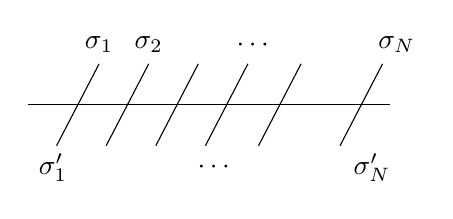
\begin{tikzpicture}[baseline=-0.5ex,x=0.9cm,y=0.8cm]
\draw (0,0)--(5.1,0);
\draw (0.4,-0.65)--(1.0,0.65);
\draw (1.1,-0.65)--(1.7,0.65);
\draw (1.8,-0.65)--(2.4,0.65);
\draw (2.5,-0.65)--(3.1,0.65);
\draw (3.25,-0.65)--(3.85,0.65);
\draw (4.4,-0.65)--(5.0,0.65);
\node at (1.0,0.95) {$\sigma_1$};
\node at (1.7,0.95) {$\sigma_2$};
\node at (3.2,0.95) {$\cdots$};
\node at (5.2,0.95) {$\sigma_N$};
\node at (0.35,-1.0) {$\sigma_1'$};
\node at (2.65,-1.0) {$\cdots$};
\node at (4.85,-1.0) {$\sigma_N'$};
\end{tikzpicture}
\end{adjustbox}
\tag{52}
\end{equation}

\begin{equation}
[\hat T_j,\hat T_{j'}]=0
\tag{53}
\end{equation}
(следствие ур-й $\triangle$-ков)
$\Rightarrow$ непротиворечивость (47)

\underline{Диагонализация $\hat T$}
(ленинградцы придумали наиболее адекватный метод)

Первый решил Янг в 1967 г.
Фаддеев и др. в 1978 г. начали заниматься.
Они проще Янга, но всё равно громоздко.

$\hat T$ \underline{соотв. опер. Лакса} $L$
([Зачёркнуто: \Unclear{GELFAND-P001161}{lax-cancelled-word}{неразборчиво}.]
это квантовое обобщение опер. Лакса $L$)

\begin{equation}
S_{\sigma_1\sigma_2}^{\sigma_1'\sigma_2'}(k)
=b(k)I+c(k)\hat P
=\begin{pmatrix}
b+\frac12c+\frac12c\sigma^z & c\sigma^- \\
c\sigma^+ & b+\frac12c-\frac12c\sigma^z
\end{pmatrix}.
\tag{54}
\end{equation}
где
\begin{equation*}
\sigma_z=\begin{pmatrix}1&0\\0&-1\end{pmatrix},
\qquad
\sigma^+=\begin{pmatrix}0&1\\0&0\end{pmatrix}
\end{equation*}
([Зачёркнуто: \Unclear{GELFAND-P001161}{pauli-cancelled-abbreviation}{м.?};
над строкой вставлено: матр.] Паули)

Табличка в пр-ве
[Зачёркнуто: \Unclear{GELFAND-P001161}{cancelled-upper-indices}{верхн.?};
над строкой вставлено: нижних.]
индексов

Матрицы $\sigma^{\pm},\sigma_z$ [Зачёркнуто: (Паули).]
действ. в пр-ве верхних индексов.

\begin{equation}
\begin{adjustbox}{max width=\linewidth}
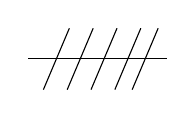
\begin{tikzpicture}[baseline=-0.5ex,x=0.55cm,y=0.6cm]
\draw (0,0)--(3.2,0);
\draw (0.35,-0.65)--(0.95,0.65);
\draw (0.9,-0.65)--(1.5,0.65);
\draw (1.45,-0.65)--(2.05,0.65);
\draw (2.0,-0.65)--(2.6,0.65);
\draw (2.4,-0.65)--(3.0,0.65);
\end{tikzpicture}
\end{adjustbox}
=\prod_i S_{ji}(k_j-k_i)
=\begin{pmatrix}A&B\\C&D\end{pmatrix}
\tag{55}
\end{equation}
(запись, учит. открытые хвосты)

$\underline{k_j=k}$ выделен.
(аналог спектр. пар. в предст. Лакса)

\begin{equation}
\begin{pmatrix}A(k)&B(k)\\C(k)&D(k)\end{pmatrix}
=\prod_i S_{*i}(k-k_i)
\qquad
\begin{adjustbox}{max width=\linewidth}
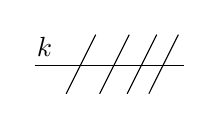
\begin{tikzpicture}[baseline=-0.5ex,x=0.5cm,y=0.6cm]
\draw (0,0)--(3.8,0);
\draw (0.8,-0.6)--(1.55,0.65);
\draw (1.65,-0.6)--(2.4,0.65);
\draw (2.35,-0.6)--(3.1,0.65);
\draw (2.9,-0.6)--(3.65,0.65);
\node at (0.25,0.4) {$k$};
\end{tikzpicture}
\end{adjustbox}
\tag{56}
\end{equation}

$T(k)\otimes T(k')$

Все шпалы можно переносить через точку пересеч. линий (ур-е $\triangle$-ков)

\begin{center}
\begin{adjustbox}{max width=\linewidth}
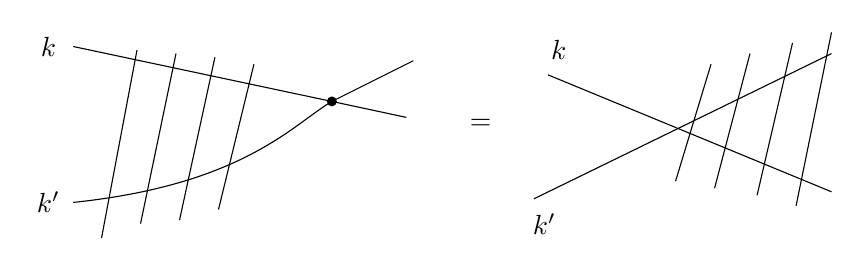
\begin{tikzpicture}[x=0.9cm,y=0.9cm]
\draw (0,1.1)--(3.65,0.325)--(4.7,0.1);
\draw (0,-1.1).. controls (2.4,-0.85) and (3.1,0) .. (3.65,0.325)--(4.8,0.9);
\draw (0.4,-1.6)--(0.9,1.05);
\draw (0.95,-1.4)--(1.45,1.0);
\draw (1.5,-1.35)--(2.0,0.95);
\draw (2.05,-1.2)--(2.55,0.85);
\fill (3.65,0.325) circle (0.07);
\node at (-0.35,1.1) {$k$};
\node at (-0.35,-1.1) {$k'$};
\node at (5.75,0) {$=$};
\draw (6.7,0.7)--(10.7,-0.95);
\draw (6.5,-1.05)--(10.7,1.0);
\draw (8.5,-0.8)--(9.0,0.85);
\draw (9.05,-0.9)--(9.55,1.0);
\draw (9.65,-1.0)--(10.15,1.15);
\draw (10.2,-1.15)--(10.7,1.3);
\node at (6.85,1.05) {$k$};
\node at (6.65,-1.4) {$k'$};
\end{tikzpicture}
\end{adjustbox}
\end{center}

\begin{equation}
T(k)\otimes T(k')\cdot S(k-k')
=S(k-k')T(k')\otimes T(k)
\tag{57}
\end{equation}

Получ. коммутац. соотн. между элементами $A,B,C,D$.
Они имеют вид:

\SourcePage{GELFAND-P001162}{unlabelled}
% Review coordinates: original pixels, upper-left origin;
% rectangles are (x0,y0,x1,y1). Enlargements add no source pixels.
% 1162-top: original page P001162; crop (x0,y0,x1,y1)=(125, 75, 1870, 660); displayed at 3x.
% 1162-vector: original page P001162; crop (x0,y0,x1,y1)=(135, 660, 1830, 1185); displayed at 3x.
% 1162-middle: original page P001162; crop (x0,y0,x1,y1)=(130, 1180, 1460, 1810); displayed at 3x.
% 1162-states: original page P001162; crop (x0,y0,x1,y1)=(120, 1800, 2030, 2445); displayed at 3x.
% 1162-bottom: original page P001162; crop (x0,y0,x1,y1)=(125, 2425, 2250, 3350); displayed at 3x.
% 1162-eq60-indices: original page P001162; crop (x0,y0,x1,y1)=(575, 885, 1225, 1060); displayed at 8x.
% 1162-eq64-index: original page P001162; crop (x0,y0,x1,y1)=(630, 2100, 830, 2220); displayed at 10x.
% 1162-cancel-word: original page P001162; crop (x0,y0,x1,y1)=(470, 2685, 683, 2768); displayed at 10x.
% 1162-insert-reference: original page P001162; crop (x0,y0,x1,y1)=(755, 2640, 965, 2775); displayed at 8x.
% 1162-eq67-exponent: original page P001162; crop (x0,y0,x1,y1)=(385, 3120, 610, 3265); displayed at 8x.
% 1162-eq62-c: original page P001162; crop (x0,y0,x1,y1)=(820, 1540, 1140, 1705); displayed at 8x.

\underline{Коммут. соотношения в элементах $A,B,C,D$:}

\begin{equation}
[A(k),A(p)]=[D(k),D(p)]=0
\tag{58}
\end{equation}

\begin{equation}
b(k-p)A(k)B(p)=B(p)A(k)-c(k-p)B(k)A(p)
\tag{59}
\end{equation}
и аналогично ещё одно.

Здесь $b(k),c(k)$ те же, что в (54).

Рассм. вектор
\begin{equation}
\Omega=f_{\sigma_1',\sigma_2'}
=\delta_{\sigma_1'1}\delta_{\sigma_2'1}
=\Unclear{GELFAND-P001162}{eq60-vector-dimension}{\begin{pmatrix}1\\0\end{pmatrix}}
\tag{60}
\end{equation}

$S$-матр. [Вставлено над строкой: (54).]
на векторе $\Omega$ становится треугольной

Отсюда Произв. $S$-матриц имеет соб. вектор
\begin{equation}
\Omega=\begin{pmatrix}1\\0\end{pmatrix}
\otimes\begin{pmatrix}1\\0\end{pmatrix}\otimes\ldots
\tag{61}
\end{equation}

Поскольку
\begin{equation}
b=\frac{k}{k+ic},\qquad c=\frac{ic}{k+ic}
\tag{62}
\end{equation}
(из унитарности и пр.),

\begin{equation}
\text{то находим соб. значение:}\quad
\underline{b(k-k_1)b(k-k_2)\ldots}
\qquad\text{\Unclear{GELFAND-P001162}{eq63-source-question}{(?)}}
\tag{63}
\end{equation}

Другие соб. векторы: ищем их в виде
\begin{equation}
\Omega(\lambda_1,\ldots,
\text{\ReaderApparatusRef{1}{1}})
=B(\lambda_1)\ldots B(\lambda_N)\Omega
\tag{64}
\end{equation}
[Под последним $\Omega$, с указателем: вакуум.]

Теперь подбираем $\lambda_1,\ldots,\lambda_N$.

\begin{equation}
\Omega\text{ — соб. для }A\text{ с соб. знач. }1
\tag{65}
\end{equation}

Применяем $A$ и пользуемся коммут. соотношениями
$\Rightarrow$ для 1-го члена всегда собств.;

Для [Зачёркнуто: \Unclear{GELFAND-P001162}{cancelled-before-second-term}{неразборчиво}.]
2-го [Вставлено над строкой: в (59).] уже не так ("unwanted terms")

Соб. значения:
\begin{equation}
T=\prod_{\alpha}\frac{1}{b(k_j-\lambda_{\alpha})}
\tag{66}
\end{equation}

Итого:
\begin{equation}
e^{2ik_jL}=\prod_{\alpha=1}^{M}
\frac{k_j-\lambda_{\alpha}+ic}{k_j-\lambda_{\alpha}-ic},
\qquad j=1,\ldots,N.
\tag{67}
\end{equation}

\ReaderNotesStart{GELFAND-P001162}
\ReaderNote{1}{\Unclear{GELFAND-P001162}{eq64-overwritten-index}{$\lambda_M$}}
\ReaderNotesEnd
\SourcePage{GELFAND-P001163}{46}
\begin{equation*}
\prod_{j=1}^{N}\left(\frac{\lambda_\alpha-k_j+ic}{\lambda_\alpha-k_j-ic}\right)
=\prod_{\beta=1}^{M}\left(\frac{\lambda_\alpha-\lambda_\beta+i2c}{\lambda_\alpha-\lambda_\beta-i2c}\right),
\qquad \alpha=1,\ldots,M. \tag{68}
\end{equation*}
Получ. разложение опер. в серию Клебша--Гордана
\begin{equation*}
\square\times\square\times\cdots\times\square
=\sum\ \tikz[baseline=-2pt]{\draw (0,0)--(0,.32)--(.65,.32)--(.65,.13)--(.35,.13)--(.35,0)--cycle;}
\end{equation*}
\underline{Это алгебр. ур-я на} $k_1,\ldots,k_N$, $E=\sum k_j^2$.

$\lambda_j$ --- вспомогательные числа, подлеж. определению.

\underline{Надо найти $\lambda$ и $k$ из (67)--(68).}
(а нужны лишь $k$)

Хотим изучить предел при $\begin{gathered}N\to\infty,\\ M\to\infty.\end{gathered}$

В пределе они решаются!!

Янг. док. разрешимость этих ур-й,
число решений --- $2^N$ и т. д.

В пределе --- интегр. ур-я,
краевые задачи и т. д.

\SourcePage{GELFAND-P001164}{56}
[В левом верхнем углу: $\downarrow$.]

\underline{20/II-84 г.}\quad \underline{Чередник.}\quad
\underline{Нелинейная теория представлений}

$\mathfrak g$ --- алг. Ли над $\mathbb C$,\quad
$U_{\mathfrak g}$ --- универс. обёрт. алг.
\begin{equation*}
U_{\mathfrak g}=\sum x_{i_1}\cdots x_{i_k},\quad x_j\in\mathfrak g.
\qquad
U_n=\left\{\sum_{x_j\in\mathfrak g}x_1\cdots x_n\right\}.
\end{equation*}
\begin{equation*}
\operatorname{Gr}=\bigoplus U_n/U_{n-1}=S^\infty(\mathfrak g)
\end{equation*}
(коммут. алг., порожд. $\mathfrak g$ как вект. пр-вом)
\begin{equation*}
[U_n,U_m]\subset U_{n+m-1}\quad\Rightarrow\quad
\operatorname{Gr}\text{ коммутативна}.
\end{equation*}
$[\quad]$ порожд. скобку Пуассона на $S^\infty(\mathfrak g)$.
(«квазиклассический предел»)

Новое опред.
\begin{equation*}
\{\ U\text{ --- градуир. [под строкой вписано: и фильтров.] со структ. по пар. }\hbar\ \}
\end{equation*}
1. Алг. Замолодчикова.

2. Алг. Склянина.

3. О нек-рых [вписано: конечн.] предст.
\begin{equation*}
\mathfrak g=\mathfrak{gl}_n,\qquad
V=\bigoplus_{\substack{\alpha\in\mathbb Z_n^2\\\lambda\in\mathbb C}}A_\alpha(\lambda),
\qquad \mathbb Z_n=\mathbb Z/n\mathbb Z.
\end{equation*}
$A_\alpha(\lambda)$ --- символ (образующая).
[Над «образующая» вписано: базис вект. пр-ва.]

(сильно бесконечномерное)

$T(V)$ --- тенз. алгебра пр-ва $V$.

В $\mathfrak{gl}_n$ выб. базис $\{I_\alpha,\alpha\in\mathbb Z_n^2\}$
(пока любой).
\begin{equation*}
L(\lambda)=\sum_{\alpha\in\mathbb Z_n^2}A_\alpha(\lambda)I_\alpha
\in\mathfrak{gl}_n(T(V)).
\end{equation*}
(матрица \Unclear{GELFAND-P001164}{matrix-word}{$n$; густо исправленный знак}
с элементами из $T(V)$)
\begin{equation*}
\overset{1}{L}=L\otimes\mathbf1,\qquad
\overset{2}{L}=\mathbf1\otimes L,\qquad
\mathbf1=\begin{pmatrix}1&&&0\\&1&&\\&&1&\\0&&&1\end{pmatrix}.
\end{equation*}
Введём матрицу [над строкой: $n^2\times n^2$]:
\begin{equation*}
R(\lambda,\mu)\in\mathfrak{gl}_n\otimes\mathfrak{gl}_n.
\end{equation*}
Соотн. на $A_\alpha(\lambda)$:
\begin{equation*}
R(\lambda,\mu)\overset{1}{L}(\lambda)\overset{2}{L}(\mu)
=\overset{2}{L}(\mu)\overset{1}{L}(\lambda)R(\lambda,\mu). \tag{1}
\end{equation*}
\begin{equation*}
\overset{1}{L}(\lambda)\overset{2}{L}(\mu)
\ne\overset{2}{L}(\mu)\overset{1}{L}(\lambda)
\end{equation*}
(вообще говоря) из-за некоммутативности $T(V)$.

Из (1) следует, что
\begin{equation*}
A_\alpha(\lambda)A_\beta(\mu)
=\sum r_{\alpha\beta}^{\gamma\delta}(\lambda,\mu)
A_\gamma(\mu)A_\delta(\lambda). \tag{2}
\end{equation*}
($r_{\alpha\beta}^{\gamma\delta}$ не выписывается)
\qquad (матрица $R(\lambda,\mu)$ считается обратимой)

\SourcePage{GELFAND-P001165}{unlabelled}
(3) \underline{Теор.} Пусть $A=T(V)/(1)$.
[Под $(1)$: идеал, порожд. (1).]
Тогда равносильны условия

а) Все мономы $A_\alpha(\lambda_1)A_\beta(\lambda_2)\cdots A_\delta(\lambda_k)$
линейно незав. в $A$ (при фиксированных $\lambda_1,\lambda_2,\ldots,\lambda_k$
и при произв. фиксир. $k$).

б) $R$ факторизуема, т. е. вып. соотношения Янга--Бакстера или $\triangle$-ка.
\begin{equation*}
\overset{12}{R}(\lambda,\mu)\overset{13}{R}(\lambda,\nu)\overset{23}{R}(\mu,\nu)
=\overset{23}{R}(\mu,\nu)\overset{13}{R}(\lambda,\nu)\overset{12}{R}(\lambda,\mu). \tag{4}
\end{equation*}
\begin{equation*}
R=\sum\rho_{\alpha\beta}I_\alpha\otimes I_\beta
\quad\Rightarrow\quad \overset{12}{R}=R\otimes1.
\end{equation*}
[После $I_\beta$ зачёркнуто:
\Unclear{GELFAND-P001165}{cancelled-r12}{$=\overset{12}{R}$; начало записи под штриховкой}.]
\begin{equation*}
\overset{13}{R}=\sum\rho_{\alpha\beta}I_\alpha\otimes1\otimes I_\beta
\qquad\text{и аналог. }\overset{23}{R}.
\end{equation*}
\underline{Идея:} перебрасываем с пом. соотн. (1) и т. д.
\begin{equation*}
(4)\ \Rightarrow\ 
\underset{\lambda,\mu}{\overset{12}{R}}\ 
\underset{\mu,\lambda}{\overset{21}{R}}\sim1\otimes1. \tag{5}
\end{equation*}
\underline{Пример, связ. с элл. кривой $E$.}
\begin{equation*}
E\ni\kappa=\mathbb C/\underbrace{\{\mathbb Z+\tau\mathbb Z\}}_{\Lambda},
\qquad \operatorname{Im}\tau>0.
\qquad
E_n=\frac1n\mathbb Z+\frac1n\tau\mathbb Z\ \bmod\Lambda
=\mathbb Z_n^2.
\end{equation*}
\Unclear{GELFAND-P001165}{curve-letter}{В записи $E\ni\kappa=\mathbb C/\{\mathbb Z+\tau\mathbb Z\}$
буква после $\ni$: $\kappa$ или $k$.}

$w_\alpha(\lambda)$ --- ф-я, к-рая [над «ф-я»: двоякопер.]

1) имеет полюса пор. $\le1$ в точках $-\eta+E_n$;
\begin{equation*}
2)\quad w_\alpha(\lambda+\beta)
=\omega^{\alpha_1\beta_2-\beta_1\alpha_2}w_\alpha(\lambda),
\qquad \omega^n=1\quad\text{(первообр. корень)}.
\end{equation*}
[Под $\beta$ стрелкой вверх указано: $\mathbb Z_n^2=E_n$.]
\begin{equation*}
3)\quad w_\alpha(0)=1.
\end{equation*}
$w_\alpha(\lambda)$ единственна.

Пусть
\begin{equation*}
I_\alpha I_\beta=\omega^{-\alpha_2\beta_1}I_{\alpha+\beta}
\qquad\text{(такой базис выбираем)}. \tag{6}
\end{equation*}
($n=2\ \Rightarrow$ матр. Паули;

$n>2\ \Rightarrow$ диаг. $+$ элемент Кокстера
\begin{equation*}
I_{10}=\begin{pmatrix}
1&&&&\\&\omega&&&\\&&\omega^2&&\\&&&\ddots&\\&&&&\omega^{n-1}
\end{pmatrix},\qquad
I_{01}=\begin{pmatrix}0&&&1\\1&0&&\\&1&\ddots&\\&&1&0\end{pmatrix}
\end{equation*}
и дальше по св-ву (6)

\SourcePage{GELFAND-P001166}{57}
\underline{Утв.}
\begin{equation*}
R(\lambda,\mu)=\sum_{\alpha\in\mathbb Z_n^2}
w_\alpha(\lambda-\mu)I_\alpha\otimes I_\alpha^{-1}. \tag{7}
\end{equation*}
Удовл. соотн. Янга--Бакстера (теор. Белавина).

Другой пример
\begin{equation*}
R=1\otimes1\frac{\lambda-\mu}{\eta+\lambda-\mu}
+\frac{\eta}{\lambda-\mu+\eta}P,\qquad
P=\frac1n\sum_{\alpha\in\mathbb Z_n^2}I_\alpha\otimes I_\alpha^{-1}. \tag{8}
\end{equation*}
[Во втором знаменателе $-\mu$ вписано снизу со знаком вставки.]

(9) \underline{Утв.}
$A_\alpha(\lambda)=w_\alpha(\lambda)I_\alpha^{-1}$
$\Rightarrow$ получ. конечномерное представление
$\mathcal A_R\to\mathfrak{gl}_n$.

\Unclear{GELFAND-P001166}{overhead-marks}{Над правой частью формулы (9) проведены две отдельные
горизонтальные черты, приблизительно над $w_\alpha$ и над $I_\alpha^{-1}$;
их значение неясно.}

\underline{Опр.} Алг. Склянина.
\begin{equation*}
L(\lambda)=\sum_{\alpha\in\mathbb Z_n^2}S_\alpha w_\alpha(\lambda)I_\alpha,
\qquad A_\alpha(\lambda)=S_\alpha w_\alpha(\lambda). \tag{10}
\end{equation*}
Разумные соотн.
\begin{equation*}
\sum_{\alpha,\beta}\ell_{\alpha\beta}S_\alpha S_\beta=0.
\end{equation*}
[Под $\ell_{\alpha\beta}$: $\mathbb C$, стрелка вверх к коэффициенту.]
\begin{equation*}
W=\bigoplus_{\alpha\in\mathbb Z_n^2}\mathbb C S_\alpha.
\end{equation*}
\underline{Важно:} есть серия кон.-мерных предст.
(Склянин: ФА 16:4, 17:4).

\underline{$n=2$}\qquad $S_0,S_1,S_2,S_3$
\begin{equation*}
[S_i,S_j]=\{S_0,S_k\},\qquad
[S_i,S_0]=J_i\{S_j,S_k\}.
\end{equation*}

\SourcePage{GELFAND-P001167}{unlabelled}
\underline{27/II-84 г.}\qquad \underline{Сем. Гельфанда.}

\underline{А. Зелевинский}\quad (совм. раб. с И. М. Гельфандом)

\underline{Модели представлений классич. групп и их скрытые симметрии.}

1. Все предст. $SO_3$ реализ. в ф-ях на $S^2$ (в $L^2(S^2)$).

2. L. C. Biedenharn, D. Flath:

В модели предст. $SU_3$ загадочным образом действует
$\overset{=}{s}\overset{=}{o}_8$ (только алгебра!)
и соотв. предст. $so_8$ неприводимо.

3. Первый шаг в твисторной конструкции Пенроуза
\begin{equation*}
\mathbb R^4\subset\mathbb C^4\subset G_2^4.
\end{equation*}
Содерж. \Unclear{GELFAND-P001167}{work-word}{$4$; густо исправленный знак} раб.:
все 3 конструкции перен. на все классич. группы $\Rightarrow$

$\Rightarrow$ сами возникают \underline{супер}группы, \underline{супер}алгебры и т. д.!!

1. Вместо компактных групп будут комплексные алгебраические

\underline{Модель:} прямая сумма всех конечномерных неприв. предст. по одному разу
\begin{equation*}
\begin{array}{c|c|c||l}
GL(n,\mathbb C)&O(n,\mathbb C)&Sp(2n,\mathbb C)&\text{комплексные}\\
U(n)&O(n,\mathbb R)&U(n,\mathbb H)&\text{компактные}
\end{array}
\end{equation*}
$G$ --- одна из групп $GL(n,\mathbb C)$, $O(n,\mathbb C)$, $Sp(2n,\mathbb C)$.

1 реализация: индуц. представление (в ф-ях или в сеч. рассл. на однородном пр-ве $G/M$).

\SourcePage{GELFAND-P001168}{60}
\begin{equation*}
\operatorname{Ind}_M^G\tau
\end{equation*}
Модель (Бернштейн $+$ 2 Гельфанда):
\begin{equation*}
\begin{array}{c||c|c|c|c}
G&GL(n)&O(2n+1)&O(2n)&Sp(2n)\\
M&O(n)&O(n+1)\times O(n)&O(n)\times O(n)&GL(n)\\
\tau&\lambda(n)&\lambda(n+1)\otimes1&\lambda(n)\otimes1&\lambda(n)
\end{array} \tag{1}
\end{equation*}
(всё комплексное)

$\lambda(n)$ --- внешняя алгебра стандартного представления

(на самом деле из-за супергрупп)

\underline{Двойств. модели}\qquad (супердвойств.)
\begin{equation*}
\begin{array}{c||c|c|c|c}
G&GL(2n)&O(2n)&Sp(4n+2)&Sp(4n)\\
M&Sp(2n)&GL(n)&Sp(2n+2)\times Sp(2n)&Sp(2n)\times Sp(2n)\\
\tau&\sigma(2n)&\sigma(n)&\sigma(2n+2)\otimes1&\sigma(2n)\otimes1
\end{array} \tag{2}
\end{equation*}
Здесь $\sigma(n)$ --- симметрическая алгебра стандартного представления.

(3) \underline{Переход:}
\begin{equation*}
\begin{aligned}
G(n)&\longrightarrow GL(2n)\\
O(n)&\longrightarrow Sp(2n)\\
Sp(2n)&\longrightarrow O(4n)\\
\lambda(n)&\longrightarrow\sigma(2n)
\end{aligned}
\end{equation*}
\Unclear{GELFAND-P001168}{transition-g}{В первой строке слева написано $G(n)$;
возможный пропуск $L$ в источнике.}

(4) \underline{Теорема 1.}\quad \underline{Табл. (2) сост. из моделей.}

\underline{Замеч.} В ней не все классич. группы (в отличие от (1)):
нет $GL(2n+1)$ и $O(2n+1)$; это будет после комментариев.

$G\subset L$ --- надгруппа.\qquad $L$ --- тоже группа.

Модель в смысле \underline{надгруппы}:
в [зачёркнуто: \Unclear{GELFAND-P001168}{model-cancelled}{$M$; неразборчивый фрагмент};
вписано снизу и обведено: модели] действует предст. алг. Ли $\ell$ группы $L$.

Модели строятся по одной геом. схеме.

$\Gamma(L)$ --- основной грассманиан группы $L$.

\underline{И. М. Г.} Замеч. объект $G_2^4$ --- о нём надо написать книгу
(основной кирпичик).

Вообще \Unclear{GELFAND-P001168}{grassmann-index}{$G_{2n}^{2n}$; возможно, $2$ в нижнем индексе отменено: $G_n^{2n}$}
--- основное.

Какие есть многогранники?

Что заменяет их объёмы?

Откуда дилогарифм?

Хар. классы и почему они не локализуются, что заменяет локализацию?

См. \underline{средневек.} книгу про \underline{икосаэдр}
(и кн. Клейна об этом).

\SourcePage{GELFAND-P001169}{unlabelled}
\underline{А. З.} Список грассманианов (они однор. пр-ва соотв. группы):
\begin{equation*}
\left[\begin{aligned}
\Gamma(GL(2n))&=\Gamma_n^{2n}\\
\Gamma(GL(2n+1))&=\Gamma_{n+1}^{2n+1}\\
\Gamma(O(2n))&=\text{грассманиан $n$-мерных изотропных подпр-в в $\mathbb C^{2n}$}\\
&\quad\text{(изотр. --- все векторы имеют 0-ю длину)}\\
&\quad\text{Он несвязен.}\\
\Gamma(O(2n+1))&=\text{грассманиан $n$-мер. изотропных подпр-в в $\mathbb C^{2n+1}$}
\end{aligned}\right. \tag{5}
\end{equation*}
[К первой строке справа: $n$-мерные плоск. в $2n$-мерном пр-ве.]

В $\mathbb C^2$: $z_1^2+z_2^2=0$, $z_1=\pm iz_2$
$\Rightarrow$ $\Gamma(O(2))$ состоит из 2-х точек.

(6) \underline{Упражнение.} Отобр.
\begin{equation*}
\begin{adjustbox}{max width=\linewidth}
\begin{tikzcd}[column sep=large]
\Gamma(O(2n))\arrow[d]&L\arrow[d,mapsto]\\
\Gamma(O(2n-1))&L\cap\mathbb C^{2n-1}
\end{tikzcd}
\end{adjustbox}
\end{equation*}
изоморфно на каждой компоненте.

(5) [продолж.]
$\Gamma(Sp(2n))$ --- грассманиан $n$-мерных лагранжевых подпр-в в $\mathbb C^{2n}$.

Дальше: \underline{$G\subset L$.}

$\Gamma(L)\supset\Omega$.
[Под $\Omega$: откр. подмн-во (чтобы были голом. ф-и).]

В ф-ях на $\Omega$ [зачёркнуто:
\Unclear{GELFAND-P001169}{omega-cancelled}{р\ldots; остальное неразборчиво}]
и строится представление.

$\Omega$ --- единственная открытая орбита.

$L$ не действует, но $\ell$ действует
[зачёркнуто: \Unclear{GELFAND-P001169}{acts-cancelled}{неразборчивый знак}]
в ф-ях на [зачёркнуто: \Unclear{GELFAND-P001169}{before-omega}{$\ell$; неразборчивый знак}]
$\Omega$ (инфинитезим. сдвиги!).

\underline{И. М. Г.} Видимо, есть чётный дифференциал вместо $d$ (с $d^2=0$).
\begin{equation*}
\begin{array}{c|c|c|c}
\widetilde L&OSp(2\vert2n)&GL(2n+\varepsilon\vert1)&OSp(2\vert2n)\times Sp(2n)\\
\widetilde\pi&\Lambda(2n)&\Lambda(2n+\varepsilon)&\Lambda(2n)\otimes1\\
L&Sp(2n)&GL(2n+\varepsilon)&Sp(2n)\times Sp(2n)\\
G&GL(n)&O(2n+\varepsilon)&Sp(2n)\\
M&O(n)&O(n+\varepsilon)\times O(n)&GL(n)\\
\tau&\lambda(n)&\lambda(n+\varepsilon)\otimes1&\lambda(n)
\end{array} \tag{7}
\end{equation*}
$\varepsilon=0,1$.

[Справа от таблицы:]
$\Omega=G/M$.

$\tau$ --- предст. в слое.
\begin{equation*}
\operatorname{Ind}_M^G\tau.
\end{equation*}
(8) \underline{Теор.} При действии $G$ на $\Gamma(L)$ имеется единств. открытая орбита
и вект. расслоение $\pi$ и в нём действует $\ell$ (скрытая симметрия).

Предст. «почти» неприводимо.

\SourcePage{GELFAND-P001170}{61}
\begin{equation*}
\begin{array}{c|c|c|c|c}
L&SO(2n+2)&O(2n+2)\times SO(2n+2)&SO(2n+2)\times O(2n)&GL(2n+1)\\
G&GL(n)&O(2n+1)&O(2n)&Sp(2n)\\
M&&\text{---}&GL(n)&\text{[зачёркнуто]}\\
M_0&Sp(n-1)&GL(n)&GL(n-\frac12)&Sp(n)\times Sp(n-1)
\end{array}\tag{9}
\end{equation*}
[При последнем столбце:] $\pi$ здесь тривиально (реализация в ф-ях на грассманиане).

[Зачёркнутая ячейка строки $M$, последний столбец:]
\Unclear{GELFAND-P001170}{table-m-cancelled}{$GL(n)$?}

\Unclear{GELFAND-P001170}{table-ranks}{В строке $M_0$ сохранены видимые $Sp(n-1)$, $GL(n-\frac12)$ и $Sp(n)\times Sp(n-1)$.}

[Зачёркнуто:] \Unclear{GELFAND-P001170}{cancelled-theorem}{(10) Теор.}
\begin{equation*}
\tau=\operatorname{Ind}_{M_0}^{M}1
\quad\Rightarrow\quad
\text{в табл. (7) написано }\operatorname{Ind}_{M_0}^{G}1.
\end{equation*}
$\Rightarrow$ на самом деле на $L$ возник. пучок $\widetilde L$
$\Rightarrow$ \Unclear{GELFAND-P001170}{super-word}{супермн-ие; супермн-зе}
и суперграссманиан.

[Зачёркнуто: \Unclear{GELFAND-P001170}{before-est}{неразборчивое сокращение}.]
Есть много необычн. симметрий; например: верхн. строка (9) похожа на нижнюю в (7).

\underline{И. М. Г. Нерешенный вопрос.}
На $G/M$ действ. большая гр. симметрий.
Какие есть ещё симметрии?

[Под заголовком зачёркнута строка, начинающаяся с «а)»:]
\Incomplete{GELFAND-P001170}{cancelled-question}{Отменённая строка не читается полностью: возможные фрагменты «найти» и «такую», между ними слово скрыто плотной правкой.}

\underline{Никифоров.} (совм. с Уваровым и Сусловым)
\begin{equation*}
\sigma(x)y''+\tau(x)y'+\lambda y=0,\tag{1}
\end{equation*}
$\sigma$ --- мног. 2-й степ.,
$\tau$ --- мног. степ. $\leq1$-й.

При
\begin{equation*}
\lambda=\lambda_n=-n\tau'-\frac{n(n-1)}2\sigma''\tag{2}
\end{equation*}
--- ортог. полиномы.

Многие спец. ф-и здесь содержатся:
\begin{equation*}
P_n^{(\alpha,\beta)}(x),\quad L_n^\alpha(x),\quad H_n(x)
\end{equation*}
(ортог. полиномы), в завис. от степ.

Общ. ф-ла:
\begin{equation*}
y_n(x)=\frac{A_n}{\rho(x)}\frac{d^n}{dx^n}
[\sigma^n(x)\rho(x)].\tag{3}
\end{equation*}
$\rho$ --- из ур-я: $(\sigma\rho)'=\tau\rho$.

[Справа:] Здесь сидит вся теория спец. ф-й --- гипергеом., вырожд. гипергеом. и т. д.
Надо взять \underline{$n$ нецелое}.
\begin{equation*}
y(x)=\frac{A}{\rho(x)}\frac1{\Gamma(\alpha)}
\int\frac{\sigma^\alpha(s)\rho(s)}{(s-x)^{\alpha+1}}.\tag{4}
\end{equation*}
$\alpha$ из соотн. типа (2).

\SourceFigure{GELFAND-P001170}{integral-contour}{Под интегралом (4) нарисована петля справа с двумя незамкнутыми ветвями влево; над верхним изгибом плотные косые штрихи. Направление обхода и значение штрихов не установлены.}

(5) [Зачёркнуто двумя пересекающимися линиями:]
\begin{equation*}
\frac{\sigma^{\alpha+1}(s)\rho(s)}{(s-x)^{\alpha+2}}.
\end{equation*}
Св-во (1): ур-е для $y'$ имеет тот же вид!! (с другими пар.)

\underline{Обобщ.:} переход к разностному ур-ю с сохр. св-ва (5).

[На левом поле зачёркнуто: \Unclear{GELFAND-P001170}{bottom-left-cancelled}{В\ldots}.]

\underline{И. М. Г.} Что такое многомерная гипергеом. функция?
Пробовали И. М. Г., Гиндикин и т. п.

[Зачёркнуто: \Unclear{GELFAND-P001170}{before-condition}{неразборчивое короткое слово}.]
\Unclear{GELFAND-P001170}{condition-word}{Усл.:}
чтобы матрич. элементы через неё писались (через монодромию).

\underline{Н.}
\begin{equation*}
\begin{aligned}
&\tau(x)\frac12\left[
\frac{y(x+h)-y(x)}h+\frac{y(x)-y(x-h)}h
\right]+\lambda y(x)\\
&\qquad+\sigma(x)\frac12\left[
\frac{y(x+h)-y(x)}h-\frac{y(x)-y(x-h)}h
\right]=0.
\end{aligned}\tag{6}
\end{equation*}
\Unclear{GELFAND-P001170}{difference-prefactor}{Перед второй квадратной скобкой в (6) написано $\frac12$.}

\SourcePage{GELFAND-P001171}{unlabelled}
$\Rightarrow$ получ. полиномы дискр. переменной.

Вместо полин. Якоби --- возник. полин. Хана
$h_n(x)$ или $h_n^{(\alpha,\beta)}(x,N)$
$\left(\frac2N=h\right)$.

Они ортог. с весом на дискр. мн-ве точек.

$\Rightarrow$ коэфф. Клебша--Гордана.
\begin{equation*}
(-1)\quad
\langle j_1m_1\; j_2m_2\mid jm\rangle
=\frac{\sqrt{\rho(x)}}{d_n}h_n^{(\alpha,\beta)}(x,N).
\end{equation*}
\Unclear{GELFAND-P001171}{minus-one}{Слева от формулы стоит $(-1)$ без видимого показателя степени.}
\begin{equation*}
\begin{gathered}
n=j-m,\quad x=j_2-m_2,\quad N=j_1+j_2-m+1,\\
\alpha=m-m',\quad\beta=m+m',\quad m'=j_1-j_2.
\end{gathered}
\end{equation*}
Вес
\begin{equation*}
\rho(x)=\frac{\Gamma(\alpha+N-1)\Gamma(\beta+x+1)}
{\Gamma(x+1)\Gamma(N-x)}.
\end{equation*}
\Unclear{GELFAND-P001171}{weight-argument}{В первом множителе числителя написано $\Gamma(\alpha+N-1)$.}

В кн. \underline{Гельф.--Минл.--Шапиро} --- выраж. через полиномы Якоби.
Но там ф-ла --- полином зав. от $n$ (?)

(\Unclear{GELFAND-P001171}{incorrect-word}{неверное; неверно} $\rho(x)$)

Можно перейти к переменной сетке и так записать разн. опер., чтобы из полиномов
получ. полиномы соотв. степеней.

Квадр. сетка даёт коэфф. Рака вместо Клебша--Гордана.

\SourcePage{GELFAND-P001172}{66}
\underline{5/III--84 г.}\qquad \underline{Сем. Гельфанда.}

[Зачёркнуто: \Unclear{GELFAND-P001172}{cancelled-name}{Фрадкин}.]
\underline{Березанский Ю. М.}

\underline{Приложения обычной спектр. обр. задачи вместо обр. зад. теории рассеяния.}
\begin{equation*}
\left\{
\begin{aligned}
\dot a_n&=\frac12 a_n\,
\text{\ReaderApparatusRef{1}{1}}
\,b_{n+1}\\
\dot b_n&=a_n^2-a_{n-1}^2
\end{aligned}
\right.\tag{1}
\end{equation*}
(цеп. Тода)

$n=0,1,\ldots$

$a_{-1}=0$.

[Справа:]
\begin{equation*}
a(t)=(a_0(t),a_1(t),\ldots)
\end{equation*}
\begin{equation*}
b(t)=b_0(t),b_1(t),\ldots)
\end{equation*}
\Unclear{GELFAND-P001172}{b-vector-bracket}{В строке $b(t)$ перед $b_0(t)$ открывающая скобка не видна; конечная скобка сохранена.}

$a(0),b(0)$ известны.

\underline{В классе посл.:}
$a(t)\in\ell^\infty$, $b(t)\in\ell^\infty$; $\forall t$ и $a_j(t)>0$.

\underline{Утв.} Реш. сущ., единств. и получ. след. процедурой:

Рассм. матр. Якоби
\begin{equation*}
\begin{pmatrix}
b_0(0)&a_0(0)&&0\\
a_0(0)&b_1(0)&a_1(0)&\\
\text{[зачёркнуто]}&a_1(0)&&\\
0&&&
\end{pmatrix}=L(0).\tag{2}
\end{equation*}
[В первом столбце, третья строка, зачёркнуто:]
\Unclear{GELFAND-P001172}{matrix-cancelled}{$a_1(0)$; $a_0(0)$; индекс неразборчив.}

\begin{equation*}
\mu(t)=\left[\int_{-\infty}^{\infty}e^{\lambda t}\,d\rho(\lambda,0)\right]^{-1};\tag{3}
\end{equation*}
\underline{Теорема:}
\begin{equation*}
\fbox{$\mu(t)e^{\lambda t}d\rho(\lambda;0)=d\rho(\lambda;t)$}
\end{equation*}
при эволюции $L(t)$ в силу (1).

$\rho(\lambda,0)$ --- спектр. ф-я матр. Якоби $L(0)$.

$\rho(\lambda,t)$ --- [зачёркнутая фраза:
\Incomplete{GELFAND-P001172}{rho-cancelled-phrase}{Несколько слов и выражение, похожее на $\rho(t)$, перекрыты отменяющими штрихами; полного прочтения нет.}]
спектр. ф-я $L(t)$, её элем. $a_n(t)$, $b_n(t)$.

\underline{И. М. Г.} (пояснение)
\begin{equation*}
\int_0^\infty t^n\,d\rho(t)=a_n\qquad\text{(пусть дано)}
\end{equation*}
\begin{equation*}
\int_0^\infty P(t)\,d\rho(t)\qquad\text{известен тоже}
\end{equation*}
$\Rightarrow$ $(P,Q)_{L_\rho^2}$ известно.

\underline{Условие:} неотрицательность этого скал. произв.

Получ. гильб. пр-во и в нём умн. на $t$
$\Rightarrow$ ортогонализация, строим ортон. базис $P_n(t)$.
\begin{equation*}
tP_n(t)=a_{n-1}P_{n-1}(t)+b_nP_n(t)+a_nP_{n+1}(t).
\end{equation*}
(меньше $P_{n-1}$ нет из-за самосопр. оператора).

$\{a_n\}\rightsquigarrow$ матр. Якоби.

Матр. Якоби $\rightsquigarrow$ пробл. моментов.

Есть спектр. разложение.
\begin{equation*}
\underline{(E(\lambda)1,1)=\rho(\lambda)}
\end{equation*}
--- эта ф-я решает пробл. моментов.

Единств. и неединств. --- глубокие вещи.

Сущ. самосопр. не всегда есть!

$\rho$ неединств. $\Leftrightarrow$ опер. $L$ имеет инд. дефекта $\Leftrightarrow$

\ReaderNotesStart{GELFAND-P001172}
\ReaderNote{1}{\Unclear{GELFAND-P001172}{toda-symbol}{$(-$; $\Delta$; знак не установлен}}
\ReaderNotesEnd
\SourcePage{GELFAND-P001173}{unlabelled}
$\Leftrightarrow a_n$ не слишком быстро растёт.

Связь с квазианалит. классами и т. д.

[Зачёркнуто: Спектр. разл. самосопр. оператора.]

\underline{Ю.М.Б.} $a,b$ ограничены $\Rightarrow$ самосопряжённость.
\begin{equation*}
a_n(t)=\int_{-\infty}^{\infty}\lambda P_n(\lambda;t)P_{n+1}(\lambda,t)\,d_\lambda\rho(\lambda,t)
\end{equation*}
\begin{equation*}
b_n(t)=\int_{-\infty}^{\infty}\lambda P_n^2(\lambda,t)\,d_\lambda\rho(\lambda,t)
\end{equation*}
\underline{Разница:} без асимптотики на бесконечности!!

\underline{Условия.} $e^{tA}$ имеет смысл для исходной матр. Якоби.

\subsection*{Фрадкин Е.С. Как построить единую теорию всех взаимодействий?}
\underline{Соврем. т. зрения:}

$\exists$ широкая группа и все элем. [Зачёркнуто:
\Unclear{GELFAND-P001173}{middle-cancellation}{неразборчивое слово}]
частицы вклад. в \underline{одно} её представление.
(при больших энергиях)

Осн. частица; остальные --- её проекции.

Разруш. группы [Вставлено над строкой: (симметрии)] должно быть спонтанное.

При малых энергиях распадается.

Гравитоны тоже войдут.

Пр-во/время остаётся

рим. метрика тоже будет.

Группа будет --- супергруппа

(суперрасш. гр. Пуанкаре или конформной группы).

\subsection*{1. Объединение электромагн. и слабого взаимод.}
(Вайнберг, Салам, Глэшоу)

см. обзор: \underline{Phys. Reports}, 1981, \underline{Lancaster}.

Группа $SU(2)\times U(1)$ объединяет слабое и эл.-магн. взаимод.

Вся физика низких энергий описывается группой
\begin{equation*}
\begin{gathered}
SU(3)\times SU(2)\times U(1)\\
\downarrow\\
SU(5)
\end{gathered}
\qquad
\begin{pmatrix}e\\ \nu\end{pmatrix}_{L}
\qquad
\begin{pmatrix}u_i\\ d_i\end{pmatrix}_{L}\text{ --- кварки.}
\end{equation*}
[Справа от нижней группы:] простейшая модель, к-рая объединяет. (все векторные частицы)

\underline{И.М.Г.} (см. также обзор Коулмена в «калибр. полях»)

\underline{Супергруппа} --- расш. гр. Пуанкаре
\qquad Гольфанд, Лихтман

обзор \Unclear{GELFAND-P001173}{lower-bibliography}{Ferrari}, Fayet
\qquad Phys. Report, 1978.
\begin{equation*}
\begin{aligned}
[M,M]&=M &&\text{(лоренц)}\\
[P,M]&=P &&\text{(Пуанкаре)}\\
[Q^\alpha,\bar Q^\beta]&=i(\gamma^\mu\bar c)^\alpha_{\beta}P_\mu.
\end{aligned}
\end{equation*}

\SourcePage{GELFAND-P001174}{67}
Гравитация --- калибр. теор. гр. Пуанкаре.

\underline{Супергравитация:} обзор: \underline{Nieuwenhauzen}

Phys. Report, т. 68, $N=4$ (1981)

Больше обзоров нет.

\underline{Большое объединение} (без гравит.) --- \underline{24} --- разм. группа, в к-рой все частицы объед.

(\underline{Великое объединение} (с гравитацией))

[Слева от формулы:] Большое объед. ср. с группой:
\begin{equation*}
S^{?}U(4)\times G_k
\end{equation*}
\Unclear{GELFAND-P001174}{upper-group}{Обведённый знак между $S$ и $U(4)$ не прочитан.}
[Под $G_k$ короткая вертикальная черта и подпись:] калибров.

\underline{замеч.} [Зачёркнут знак:
\Unclear{GELFAND-P001174}{upper-cancellation}{неразборчиво}]
группа, реш. великое объед.
\begin{equation*}
G_k=E_8
\end{equation*}
(совпад. с присоед.) [Над строкой вставлено: Фундамент. предс.]

[Справа:] $E_8\supset SU(5)$ в кач. подгруппы.

Лагранжиан: Письма \underline{ЖЭТФ} т. 32, \underline{575} (Фрадкин, Конштейн)

($SU(5)$ --- «Кварки-80» (Фрадкин))

$E_8$-модель --- \underline{конечна} --- не имеет расходимостей \underline{вообще!!!} ---

--- во всех петлях

Вайнштейн, Шифман,

Фрадкин, Цейтлин --- Phys. Letters, \underline{135} (1984), стр. 302(?)

Калибрование --- искусство (техники пока нет)

По группе $G$ строим связность $V_\mu$ (или вект. поле)
\begin{equation*}
V_\mu=e_\mu^a P_a+\omega_\mu^{mn}M^{mn}+\bar\psi_\mu^\alpha\Theta_\alpha.
\end{equation*}
\Unclear{GELFAND-P001174}{connection-indices}{В первой формуле оба индекса $mn$ у $M$ написаны сверху.}
\begin{equation*}
\Lambda=\epsilon^aP_a+\lambda^{mn}M_{mn}+\bar\epsilon^\alpha\Theta_\alpha
\qquad\text{--- беск. малый}
\end{equation*}
\begin{equation*}
\left.
\begin{array}{lll}
\omega_{mn}&M_{mn}\text{ --- образ.,}&\omega_{mn}\text{ --- коэфф.}\\
e_\mu^a&P_\mu&
\end{array}\right]
\end{equation*}
Калибровать: \Unclear{GELFAND-P001174}{lower-word}{некотая / нечётная} группа и т. д.

НО: трансляции должны замениться чем-то локальным.

\underline{Гравит.:} теория частиц со спинами
$\begin{pmatrix}2\\3/2\end{pmatrix}$

гравитация --- спин 2.

\underline{И.М.Г.} считает, что пр-во не 3 и 4-мерно, а $\infty$-мерно.

\SourcePage{GELFAND-P001175}{unlabelled}
\subsection*{12/III-84 г. Сем. Гельфанда}
\subsection*{Фрадкин Е.С.}
\begin{equation*}
F_{\mu\nu}=\partial_\nu\hat A_\mu-\partial_\mu\hat A_\nu+[\hat A_\mu,\hat A_\nu]
\end{equation*}
\begin{equation*}
F_{\mu\nu}=[D_\mu,D_\nu]
\qquad
\hat A_\tau=t^a A_\tau^a
\end{equation*}
\Unclear{GELFAND-P001175}{upper-curvature}{Порядок индексов в двух записях $F_{\mu\nu}$ сохранён.}
\begin{equation*}
A'_\tau\to S(x)A_\mu S^{-1}+S\partial_\mu S^{-1}
\end{equation*}
\Unclear{GELFAND-P001175}{upper-transform-index}{Слева читается $\tau$, справа дважды $\mu$.}

Как ввести массу?

Добавка $m^2 A_\mu^2$ не годится (не калибр. инвариантно)

[Справа, стрелкой к предыдущей скобке:] и к тому же не перенормируема.

Надо за [Зачёркнуто: \Unclear{GELFAND-P001175}{middle-cancellation}{неразборчивый знак}]
счёт спонтанного наруш. симметрии.
[В конце фразы две наклонные черты.]

\underline{И.М.Г.:} надо точно сформулир., что такое перенормируемость.

Ф. \underline{Хиггс} ввёл скалярное (доп.) поле.
\begin{equation*}
(D_\tau\varphi)^2+\ldots
\end{equation*}
\begin{equation*}
\bigl((\partial_\tau^{''}+t^\alpha\hat A_\mu)\varphi\bigr)^2
\end{equation*}
\Unclear{GELFAND-P001175}{middle-derivative-marks}{Функция двух коротких штрихов после $\partial_\tau$ не установлена.}
(ковар. произв.)

Если $\langle\varphi\rangle\ne0$ (ср. по вакууму), то
\begin{equation*}
\begin{array}{cccc}
\varphi={}&C&+&\varphi'\\
&|&&\backslash\\
&\text{своб.}&&\text{конденсат}
\end{array}
\end{equation*}
\Unclear{GELFAND-P001175}{lower-field-labels}{Подписи «своб.» и «конденсат» сохранены под $C$ и $\varphi'$ соответственно.}

Получим $(t^\alpha A_\mu\varphi(0))^2$

Можно написать:
\begin{equation*}
(D_\tau\varphi)^2+m_1^2\varphi^2+\lambda\varphi^4
\end{equation*}
Варьируем:
\begin{equation*}
D_\tau^2\varphi(0)+m^2\varphi(0)+4\lambda\varphi(0)^3=0
\end{equation*}
Прост. реш. $0$

2-е реш. может быть тоже:
\begin{equation*}
m^2\varphi(0)+4\lambda\varphi(0)^3=0,\qquad
\underline{\varphi=\sqrt{\frac{-m^2}{4\lambda}}}
\quad\Rightarrow\quad\text{возникнет член массы всех частиц.}
\end{equation*}

\SourcePage{GELFAND-P001176}{71}
Лагр.
\begin{equation*}
\mathcal L=F_{\mu\nu}^2+(D_\mu\varphi)^2+m_1^2\varphi^2+\lambda\varphi^4
\end{equation*}
\underline{Хотим:} чтобы \Unclear{GELFAND-P001176}{upper-abbreviation}{остал. / оставш.} безмассовая гр. была
\begin{equation*}
SU(3)\times\underbrace{SU(2)\times U(1)}_{\text{Вайнберг--Салам}}
\end{equation*}
\begin{center}
\begin{adjustbox}{max width=\linewidth}
\begin{tikzpicture}[x=1cm,y=1cm]
\draw (0,0) .. controls (1.5,0.15) and (4,0.08) .. (6,0);
\draw (2.1,0.05) -- (2.1,1.7);
\draw (0.25,2.6) .. controls (0.6,2.15) and (1.5,1.75) .. (2.1,1.7);
\draw (0.05,1.38) .. controls (0.7,1.58) and (1.35,1.35) .. (2.1,1.7);
\draw (0.2,0.45) .. controls (1.2,0.45) and (1.65,0.85) .. (2.1,1.7);
\draw (2.1,1.7) .. controls (3.55,1.83) and (4.35,1.85) .. (5.8,0.9);
\fill (2.1,1.7) circle (0.07);
\node at (0.85,2.9) {сильное};
\node at (0.05,1.8) {сл.};
\node at (0.8,0.95) {эл.-магн.};
\node at (2.55,-0.42) {$M\sim10^{14}$ ГэВ};
\end{tikzpicture}
\end{adjustbox}
\end{center}
\begin{center}--- $\cdot$ ---\end{center}

\Unclear{GELFAND-P001176}{middle-heading}{Спис. / Случ.} с гравитацией:
\begin{equation*}
\begin{array}{llll|r}
&&&&\underline{N=8}\\
g_{\mu\nu}&\text{--- 1 частица}&&&1\\
\psi&N\text{ частиц}&(\text{из }SO(N))&(\text{спин }3/2)&8\\
A_\mu&SO(N)&(\text{векторные част.})&&28\\
\chi&&&(\text{спин }1/2)&56\\
\varphi&\text{--- скал. частицы}&&&70
\end{array}
\end{equation*}
\Unclear{GELFAND-P001176}{middle-spinor-symbol}{Символ строки со спином $1/2$ передан предположительно как $\chi$.}
$\max$ спин опред. $\underline{N/4}$ (с учётом киральности) $\Rightarrow\underline{N=8}$.

\begin{center}--- $\cdot$ ---\end{center}

В 11-мерном пр-ве возникает приличная с $N=1$ и нет \underline{конформных аномалий}.

конформ. гр.
\begin{equation*}
\left.
\begin{aligned}
[M,M]&=M\\
[P,M]&=P\\
[Q,Q]&=P\\
[D,\quad]&\\
[K,\quad]&
\end{aligned}
\right]
\quad\Rightarrow\quad\underline{\text{гравит. Вейля}}
\qquad\left(R_{\mu\nu}^{2}-\frac13R\delta_{\mu\nu}\right)
\end{equation*}
[Строка $[Q,Q]=P$ обведена; рядом:] пока без супер.
\Unclear{GELFAND-P001176}{middle-weyl-expression}{Второй член записан как $-\frac13R\delta_{\mu\nu}$.}

\underline{Простейшая задача:} вычислить интеграл
\begin{equation*}
\int e^{i\int d^4x\,R}\,dg_{\mu\nu}
\end{equation*}
сильно вырожден. \qquad квантование?

Метод Фаддеева не годится.

Фрадкин, \Unclear{GELFAND-P001176}{lower-surname}{Вилковисский} и др. ---
[Вставлено над строкой: к] гравитации и др.

Возникает ответ, не выраж. через $\det$ ---

--- скобка Ли не замкнута (замкнута только на экстремалях).

\begin{center}--- $\cdot$ ---\end{center}

\SourcePage{GELFAND-P001177}{unlabelled}
\subsection*{19/III-84 г. Сем. Гельфанда.}
\subsection*{Лейтес.}
\subsection*{Супералгебры Ли.}
$gl(n|m)$

Суперпр-во $V=V_{\bar0}\oplus V_{\bar1}$, град.
$\{\bar0,\bar1\}=\mathbb Z_2$, $\dim V=(n|m)$,
$\dim V_{\bar0}=n$, $\dim V_{\bar1}=m$.

$\operatorname{Hom}(V,W)$ --- суперпр-во;

($W$ --- другое суперпр-во $W=W_{\bar0}\oplus W_{\bar1}$)

$\operatorname{Hom}(V,W)_{\bar0}$ --- сохр. чётность;
[Под записью два коротких штриха и матрица:]
\begin{equation*}
\left\{\begin{pmatrix}A&0\\0&D\end{pmatrix}\right\}
\end{equation*}
$\operatorname{Hom}(V,W)_{\bar1}$ --- меняющие чётность.
[Под записью два коротких штриха и матрица:]
\begin{equation*}
\begin{pmatrix}0&B\\C&0\end{pmatrix}
\end{equation*}
\underline{Супералг. Ли:}
\begin{equation*}
[x,y]=-(-1)^{\bar x\bar y}[y,x]
\end{equation*}
[В начале следующей левой скобки перед $x$ зачёркнуто:
\Unclear{GELFAND-P001177}{middle-jacobi-cancellation}{неразборчивый знак}.]
\begin{equation*}
[x,[y,z]]=[[x,y],z]+(-1)^{\bar x\bar y}[y,[x,z]]
\end{equation*}
[Справа:] (правило Квиллена:)

если перест. буквы чётности $p$ и $q$, то возникает знак $(-1)^{pq}$.

Супералг.: $A=A_{\bar0}\oplus A_{\bar1}$
\begin{equation*}
m:A\otimes A\to A,\qquad p(m)=\bar0
\end{equation*}
[Справа, отделено двумя косыми чертами:] умнож. должно быть чётным.

Ассоц. супералг. $\leadsto$ \underline{супералг. Ли}
\begin{equation*}
[a,b]=ab-(-1)^{\bar a\bar b}ba
\end{equation*}
[Зачёркнуто: \Unclear{GELFAND-P001177}{lower-gl-cancellation}{неразборчивая запись}.]
$gl(n|m)$ --- супералг., получ. из $\operatorname{Hom}(\mathbb R^{n/m},\mathbb R^{n/m})$.
\begin{equation*}
sl(n|m)=\{a\mid a\in gl(n|m),\ \operatorname{str}a=0\},
\end{equation*}
\begin{equation*}
\operatorname{str}\begin{pmatrix}A&B\\C&D\end{pmatrix}=\operatorname{tr}A-\operatorname{tr}D
\end{equation*}
(эйлерова хар-ка --- суперслед)

\underline{Классиф. в обычном случае:}
[Под первым словом вставлено и подчёркнуто: алгебр.]
\begin{equation*}
gl,\ sl,\ o,\ sp,\quad w,\ S,\ H,\ K.
\end{equation*}
\begin{equation*}
osp(n|2m)=\{X\in gl(n|2m)\mid X^{st}B_{n,2m}+B_{n,2m}X=0\},
\end{equation*}
\begin{equation*}
\begin{pmatrix}A&B\\C&D\end{pmatrix}^{st}
=\begin{pmatrix}A^t&-C^t\\B^t&D^t\end{pmatrix}
\end{equation*}
(можно и $\begin{pmatrix}A^t&C^t\\-B^t&D^t\end{pmatrix}$, это эквивалентно)

\SourcePage{GELFAND-P001178}{unlabelled}
\begin{equation*}
B_{n,2m}=\left(
\begin{array}{c|c}
1_n&0\\
\rule{0.65cm}{0.3pt}&\rule{1.2cm}{0.3pt}\\
0&\begin{matrix}0&1_m\\-1_m&0\end{matrix}
\end{array}\right)
\end{equation*}
[Справа:] (чётная форма сохр.)

матрица --- \underline{чётна}.

(матрица чётной симм. \underline{или} \underline{нечётной} кососимм. формы)

\underline{И.М.Г.} изоморфная запись:
\begin{equation*}
osp(2n|2m)=\left(
\begin{array}{c|c}
\begin{matrix}0&1_n\\1_n&0\end{matrix}&0\\
\rule{1.2cm}{0.3pt}&\rule{1.2cm}{0.3pt}\\
0&\begin{matrix}0&1_m\\-1_m&0\end{matrix}
\end{array}\right)
\end{equation*}
$osp(2n+1|2m)$

\begin{center}--- $\cdot$ ---\end{center}

\underline{Л.}
\begin{equation*}
\begin{aligned}
\Pi(n)&=\{X\in gl(n|n)\mid X^{st}J_{2n}+(-1)^{\bar X}J_{2n}X=0\}\\
&=\left\{\begin{pmatrix}A&B\\C&-A^t\end{pmatrix}\;\middle|\;
\begin{gathered}B=B^t\\C=-C^t\\A\in gl(n)\end{gathered}\right\}.
\end{aligned}
\end{equation*}
[Под формулой зачёркнут фрагмент:
\Unclear{GELFAND-P001178}{upper-cancelled-aside}{неразборчиво}.]

($\Pi$ --- в честь Паламодова)
\begin{equation*}
J_{2n}=\begin{pmatrix}0&1_n\\-1_n&0\end{pmatrix}
\end{equation*}
(нечётная [Зачёркнуто:
\Unclear{GELFAND-P001178}{upper-form-cancellation}{неразборчивое слово}]
форма сохр.)

матрица нечётна.
\begin{equation*}
q(n)=\{X\in gl(n|n)\mid[X,J_{2n}]=0\}
=\left\{\begin{pmatrix}A&B\\B&A\end{pmatrix}\right\}
\end{equation*}
[От матричной записи вниз стрелка с подписью $q\cdot\operatorname{tr}$:]
\begin{equation*}
\operatorname{tr}B=\operatorname{str}(X\cdot J_{2n})
\end{equation*}
\Unclear{GELFAND-P001178}{middle-qtrace}{Равенство для $q$-следа сохранено без изменения множителя или знака.}

[Справа:] ($q$ от \underline{queer}, странный)

\underline{Вопр. И.М.Г.:} как выглядит теор. о жордановой форме?

[Зачёркнуто: \Unclear{GELFAND-P001178}{middle-sq-cancellation}{sq?}]
$sq(n)$ тоже есть.

\underline{Проективизации} есть.
\begin{equation*}
AB_3=\underbrace{sl(2)\oplus O(7)}_{(AB_3)_{\bar0}}\oplus(AB_3)_{\bar1}
\end{equation*}
[Под первым слагаемым зачёркнуты две короткие строки:
\Unclear{GELFAND-P001178}{lower-even-cancellation}{неразборчивые фрагменты}.]

У $sl(2)$ есть станд. [Вставлено сверху: 2-мерное] предст. $V$

$O(7)$ имеет предст. $\operatorname{spin}_7$ (станд.)
\begin{equation*}
V\otimes\operatorname{spin}_7\text{ --- предст. }sl(2)\oplus O(7)
\end{equation*}
\begin{equation*}
D(\alpha)=osp(4|2;\alpha)
\end{equation*}
\begin{equation*}
D(\alpha)_{\bar0}=O(4)\oplus sp(2)=sl(2)_1\oplus sl(2)_2\oplus sl(2)_3
\end{equation*}
\begin{equation*}
D(\alpha)_{\bar1}=V_1\otimes V_2\otimes V_3
\end{equation*}
$V_i$ --- станд. предст. $sl(2)_i$
\begin{equation*}
\begin{aligned}
&[v_1\otimes v_2\otimes v_3,\ u_1\otimes u_2\otimes u_3]\\
&\quad=\sum_{\substack{(i,j,k)=\\=\sigma(1,2,3)}}\lambda_k\,
\underbrace{(v_i,u_i)_i}_{\text{кососимм. произв.}}\,
(v_j,u_j)_j\,
\underbrace{v_k\cdot u_k}_{\text{симм. произв.}}
\end{aligned}
\end{equation*}
\underline{Тожд. Якоби} удовл. при: $\lambda_1+\lambda_2+\lambda_3=0$.

\SourcePage{GELFAND-P001179}{79}
\underline{Пенков И.}
\begin{equation*}
G=SL(T^{n/m})\qquad n\ne m
\end{equation*}
[Под $T$ короткая черта вниз и подпись: компл.]
[Справа зачёркнут знак: \Unclear{GELFAND-P001179}{upper-cancellation}{неразборчиво}.]

$B=$ макс. разр. замк. подсупергруппа, у к-рой все неприв.
конечномерные предст. имеют размерность $1|0$ или $0|1$.

\SourceFigure{GELFAND-P001179}{upper-borel-diagram}{Слева матричная схема в круглых скобках, с диагональю из верхнего левого в нижний правый угол и горизонтальными штрихами преимущественно над диагональю; справа подпись $B_J$. Точное значение отдельных коротких штрихов не установлено.}
\begin{equation*}
J\in\mathcal J=\{\text{перестановки }n+\text{ и }m-\}
\end{equation*}
\begin{equation*}
G/B_J=\underset{\text{(флаги)}}{Fl}(J,T^{n/m})
\end{equation*}
\begin{equation*}
\dim G/B_J=\frac{n(n-1)}2+\frac{m(m-1)}2\mid mn
\end{equation*}
$\operatorname{Pic}G/B$ --- гр. Пикара

[Под $\operatorname{Pic}$ два коротких штриха, далее:]
\begin{equation*}
\operatorname{Mor}(H,G_m)
\end{equation*}
[Под $G_m$ черта вниз:] мульт. группа
[Зачёркнуто: \Unclear{GELFAND-P001179}{middle-cancellation}{неразборчиво}]
$C^*$
\begin{equation*}
\begin{aligned}
\operatorname{Mor}(H,G_m)&\overset{\sim}{\longrightarrow}\operatorname{Pic}^{G}G/B_J
\\
&\overset{df}{=}\{\text{гр. пучков ранга }1|0\text{ с }G\text{-линеаризацией}\}
\end{aligned}
\end{equation*}
[Под $H$ черта вниз:] карт. подгр. чётной части

\underline{Теорема.}
\begin{equation*}
\begin{gathered}
\chi\in\operatorname{Mor}(H,G_m),\quad(\chi,\varepsilon_i-\varepsilon_j)\ne0,\\
(\chi,\delta_i-\delta_j)\ne0,\quad(\chi,\varepsilon_i-\delta_j)\ne0.
\end{gathered}
\end{equation*}
Тогда $\forall J$ $H^i(\mathcal O_J(\chi-\rho_J))=0$ при $i\ne l(w)$
\begin{equation*}
\begin{aligned}
H^{l(w)}(\mathcal O_{J_1}(\chi-\rho_{J_1}))
&=H^{l(w)}(\mathcal O_{J_2}(\chi-\rho_{J_2}))\\
&=V_{J_1}(\mu-\rho_{J_1})=V_{J_2}(\mu-\rho_{J_2})
\end{aligned}
\end{equation*}
$\Rightarrow$ получаются предст. со старш. весом в когомологиях.

$(\chi,\varepsilon_i-\delta_j)\ne0$, но $(\chi,\alpha_0)=0$
$\Rightarrow\forall J$ пучок $\mathcal O_J(\chi-\rho_J)$ ацикличен.

\SourcePage{GELFAND-P001180}{unlabelled}
\underline{26/III-84.}\qquad\underline{Сем. Гельфанда.}

\underline{Пенков.}
\begin{equation*}
G=SL(n|m),\qquad G/B_J=Fl(J,T)
\end{equation*}
[Справа:] $T$ --- станд. предст.,

$J$ --- индекс флага
\begin{equation*}
\operatorname{Pic}_J^G=\operatorname{Pic}^{G}(G/B_J)
\end{equation*}
\underline{Утв. 1}\qquad $\operatorname{Pic}_J^G=$ характеры $H$

\underline{Теор.} Пусть $\chi$ --- характер, $\chi$-регулярен;
[Зачёркнуто: \Unclear{GELFAND-P001180}{middle-cancellation}{неразборчивые знаки}]
$\exists\mu=w(\chi)$

[Под $\mu$ короткая черта и подпись:] доминантен

Тогда
\begin{equation*}
\forall i\quad H^i(\mathcal O(\chi-\rho_J))\quad\text{при }i\ne l(w)
\qquad\text{(длина }w\text{)}
\end{equation*}
\Unclear{GELFAND-P001180}{middle-cohomology}{Между $H^i(\mathcal O(\chi-\rho_J))$ и словом «при» в источнике нет написанного равенства или значения.}
\begin{equation*}
H^{l(w)}(\mathcal O(\chi-\rho_J))=V_J(\mu-\rho_J).
\end{equation*}
И имеется $D$-модульный вариант этой теоремы.

\underline{Аффинные флаги:} ещё с элементами площади
(\Unclear{GELFAND-P001180}{lower-parenthesis}{сопр.?}) на $\forall$ плоскости флага

$T$ --- лин. суперпр-во,
[Над следующим $T$ зачёркнут маленький знак:
\Unclear{GELFAND-P001180}{lower-t-mark}{неразборчиво}.]
\begin{equation*}
T=T^{n/m}=\underset{\text{чёт.}}{T^{n/0}}\oplus\underset{\text{нечёт.}}{T^{0/m}}
\end{equation*}
Тип.
\begin{equation*}
\begin{gathered}
T^{1/0}\subset T^{2/0}\subset\ldots\\
\subset T^{1/1}\subset\ldots
\end{gathered}
\end{equation*}
\Unclear{GELFAND-P001180}{lower-flag-type}{Размерность в последней строке прочитана предположительно как $1/1$; цифры требуют проверки.}

\SourcePage{GELFAND-P001181}{87}
\underline{Подстил. мн-ие:} произв. двух флаговых мн-ий

[Под первой частью строки:] (чётная часть)

[Под второй частью строки:] (не-зав. от типа)
\begin{equation*}
Fl(J,T)_{\text{чёт}}=Fl(1,2,\ldots,T^{n/0})\times Fl(1,2,\ldots,T^{0/m})
\end{equation*}
\begin{equation*}
\dim Fl(J,T^{n/m})=\frac{n(n-1)+m(m-1)}2\mid mn
\end{equation*}
(\underline{Из рав-ва:}
\begin{equation*}
G/B_J=Fl(J,T)
\end{equation*}
).

\begin{center}
\begin{adjustbox}{max width=\linewidth}
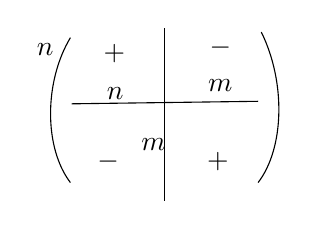
\begin{tikzpicture}[x=0.8cm,y=0.8cm]
\draw (-1.50,1.05) .. controls (-1.92,0.35) and (-1.92,-0.7) .. (-1.50,-1.25);
\draw (1.53,1.14) .. controls (1.92,0.35) and (1.90,-0.7) .. (1.48,-1.25);
\draw (-1.48,0) -- (1.48,0.04);
\draw (0,1.20) -- (0,-1.55);
\node at (-0.80,0.80) {$+$};
\node at (0.88,0.90) {$-$};
\node at (-0.90,-0.92) {$-$};
\node at (0.84,-0.92) {$+$};
\node at (-1.90,0.86) {$n$};
\node at (-0.79,0.16) {$n$};
\node at (0.88,0.29) {$m$};
\node at (-0.18,-0.65) {$m$};
\end{tikzpicture}
\end{adjustbox}
\end{center}

\SourcePage{GELFAND-P001182}{unlabelled}
\underline{2/IV-84г.}\qquad\underline{Сем. Гельфанда}

\underline{Фукс?}
\Unclear{GELFAND-P001182}{upper-speaker}{Конечные буквы фамилии или сокращения не вполне различимы.}
$\widehat{sl(2)}$ --- алгебра, порожд. 6 образующими $f_j,e_j,h_j$ $(j=1,2)$

[Под словом «алгебра»:] К.-М.

[Под обозначением алгебры два вертикальных штриха, ниже:]
\begin{equation*}
N_-\oplus H\oplus N_+
\end{equation*}
\begin{equation*}
[e_i,f_j]=\delta_{ij}h_i
\end{equation*}
\begin{equation*}
\begin{aligned}
[e_1[e_1[e_1,e_2]]]&=0\\
[e_2[e_2[e_2,e_1]]]&=0
\end{aligned}
\end{equation*}
и что-то ещё.

[Справа:]
\begin{equation*}
\begin{aligned}
[h_1,e_2]&=-2e_2,&[h_2,e_1]&=-2e_1,\\
[h_1,e_1]&=2e_1,&[h_2,e_2]&=2e_2
\end{aligned}
\end{equation*}
и такие же ф-лы с заменой $e$ на $f$

и с измен. знака.
\begin{equation*}
[h_1,h_2]=0
\end{equation*}
\underline{И.М.Г.} Эта алг. почти совп. с алгеброй
\begin{equation*}
\begin{pmatrix}a(t)&b(t)\\c(t)&d(t)\end{pmatrix},\qquad
\underline{a+d}=0,\qquad t\in S^1.
\end{equation*}
\underline{Ф.}\quad Утв. Модули Верма над ней зависят от
$2^{\underline{\text{х}}}$ компл. параметров.
$M(\lambda_1,\lambda_2)$
[Зачёркнуто: \Unclear{GELFAND-P001182}{lower-cancellation}{неразборчивый фрагмент}.]
% GELFAND-0127. Дипломатическая транскрипция; оригинальные PNG являются источником.
% Координаты проверки: (x0,y0,x1,y1), пиксели исходного PNG 2432 x 3480,
% начало координат — левый верхний угол; правая и нижняя границы исключаются.
% Zoom — коэффициент растрового увеличения ближайшим соседом, не новое разрешение.
% Все сканы просмотрены непосредственно; OCR не применялось.
% Редакторские описания в квадратных скобках не являются словами рукописи.
% Неуверенные чтения и математические замечания связаны с uncertainties.json.

\SourcePage{GELFAND-P001183}{unlabelled}
% Source image: images/GELFAND-P001183.png
% Review top-left: bbox=160,20,1060,555; zoom=3x.
% Review top-verma: bbox=940,300,2290,495; zoom=3x.
% Review upper-theorem: bbox=25,550,1885,950; zoom=3x.
% Review margin-vector: bbox=20,705,240,920; zoom=5x.
% Review theorem-attribution: bbox=180,858,1920,979; zoom=3x.
% Review weight-array: bbox=325,980,1070,1225; zoom=3x.
% Review reducibility: bbox=80,1235,1670,1682; zoom=3x.
% Review casimir-task: bbox=135,1720,1625,1925; zoom=3x.
% Review singular-vector: bbox=205,1920,2120,2177; zoom=3x.
% Review commutator: bbox=195,2160,1825,2450; zoom=3x.
% Review casimir-parenthesis: bbox=440,1810,745,1910; zoom=5x.
% Review casimir-generators: bbox=970,1810,1225,1930; zoom=5x.
% Review vector-left-exponent: bbox=450,2010,560,2100; zoom=10x.
% Review vector-right-exponent: bbox=1270,2010,1450,2150; zoom=7x.
% Review commutator-tail: bbox=1400,2290,1810,2430; zoom=5x.
% Review hodge-opening: bbox=110,2410,2360,2850; zoom=3x.
% Review hodge-bottom: bbox=90,2790,2220,3425; zoom=3x.
% Review complexification-note: bbox=1280,2600,1830,2855; zoom=4x.
% Review mixed-condition: bbox=95,3090,1170,3330; zoom=4x.
% Review attribution-name-detail: bbox=227,870,640,965; zoom=6x.
% Review singular-annihilator-detail: bbox=1255,655,1495,778; zoom=6x.
% Review mixed-bound-detail: bbox=793,3150,901,3270; zoom=10x.
% Review weight-array-bottom: bbox=328,1190,1040,1252; zoom=5x.
% Review hodge-decomposition-word: bbox=730,2985,1250,3115; zoom=4x.

$N_-$ — слова, сост. из $f_j$.

$N_+$ — слова, сост. из $e_j$.

$\dim H<\infty$.

\underline{Модуль Верма} — предст., в к-ром $\exists$ порожд. вектор, для к-рого
\begin{equation*}
\left[
\begin{aligned}
N_-v&=0\\
h_jv&=\lambda_jv
\end{aligned}
\right.
\end{equation*}
$e_1v,\quad [e_1,e_2]v,\ldots$

Может оказаться приводимым при нек-рых $\lambda_1,\lambda_2$.

\underline{Теор.} Он приводим $\Longleftrightarrow$
$\exists w\in M(\lambda_1,\lambda_2)$; $f_iw=0$.

Он тоже соб. вектор (особ. вектор).

[На левом поле: тогда $\exists w\nparallel v$.]

(Кац — \Unclear{GELFAND-P001183}{attribution-name}{Каждан / Кацдан};
$\infty$-мерн. вариант теор. Бернш. — Гельф. — Гельф.)

% Схема расположения векторов: соединяющих линий или стрелок на скане нет.
\begin{center}
\begin{adjustbox}{max width=\linewidth}
\begin{tikzpicture}
\node at (1.45,0) {$v$};
\node at (0.70,-0.70) {$e_1v$};
\node at (2.15,-0.70) {$e_2v$};
\node at (0,-1.45) {$e_1^2v$};
\node at (1.60,-1.45) {$e_1e_2v$};
\node at (3.25,-1.45) {$e_2e_1v$};
\node at (4.90,-1.45) {$e_2^2v$};
\node at (0,-2.05) {$\cdot$};
\node at (0.38,-2.05) {$\cdot$};
\node at (1.10,-2.05) {$\cdot$};
\node at (1.85,-2.05) {$\cdot$};
\node at (2.53,-2.05) {$\cdot$};
\node at (3.19,-2.05) {$\cdot$};
\node at (3.85,-2.05) {$\cdot$};
\node at (4.39,-2.05) {$\cdot$};
\node at (4.97,-2.05) {$\cdot$};
\node at (5.40,-2.05) {$\cdot$};
\node at (5.68,-2.05) {$\cdot$};
\end{tikzpicture}
\end{adjustbox}
\end{center}

\underline{Теор.} $M(\lambda_1,\lambda_2)$ приводим
$\Longleftrightarrow$ $\lambda_1,\lambda_2$ удовл. одному из ур-й
\begin{equation*}
\begin{aligned}
(1)\quad &(k+1)(\lambda_1+1)+k(\lambda_2+1)=n,\quad k\geq0,\ n\geq0.\\
(2)\quad &\lambda_1\longleftrightarrow\lambda_2\\
(3)\quad &\lambda_1+\lambda_2+2=0
\end{aligned}
\end{equation*}

\underline{Зад.} (И.М.Г.) Найти опер. Казимира этой алгебры.

(полиномы (некоммут.) от букв $e_j,f_j,$
\Unclear{GELFAND-P001183}{casimir-generator}{$l_j$ / $h_j$}
% Внешняя открывающая скобка перед словом «полиномы» не закрыта на скане.

\underline{Идея постр.:}
\begin{equation*}
w=e_1^{n+\ell t}\ldots e_2^{n+t}e_1^n e_2^{n-t}e_1^{n-2t}\ldots e_2^{n-\ell t}v
\qquad t\in\mathbb C\ (!!)
\end{equation*}

Но: оказ., что этот элемент лежит в обёрт. алгебре.
\begin{equation*}
[e_2,e_1^z]
=
ze_1^{z-1}[e_2,e_1]
+\frac{z(z-1)}{2}e^{z-2}[[e_2,e_1]e_1]+\ldots
\end{equation*}
\Unclear{GELFAND-P001183}{commutator-notation}{Во втором слагаемом индекс у $e$ и запятая между $[e_2,e_1]$ и $e_1$ не видны; после последнего плюса — два коротких штриха, переданных многоточием.}

\underline{Бейлинсон}

\underline{Структуры Ходжа.}

$n\in\mathbb Z$.

\underline{Чистая структ. Ходжа веса $n$} — $H_{\mathbb R}$,
[под $H_{\mathbb R}$: вещ. вект. пр-во]
\begin{equation*}
H_{\mathbb C}:=H_{\mathbb R}\otimes\mathbb C
=\bigoplus_{p+q=n}H^{p,q},
\qquad
\overline H^{pq}=H^{qp}.
\end{equation*}
[Под $H_{\mathbb C}$ стрелка вниз к приписке: его к.]

Фильтрация Ходжа:
\begin{equation*}
F^iH=\bigoplus_{p\geq i}H^{p,q}.
\end{equation*}

Структура по ней восстанавливается:
\begin{equation*}
H^{p,q}=F^pH\cap\overline F^{q}H.
\end{equation*}

\underline{Смеш. структ. Ходжа}\quad
$H_{\mathbb R}$ и разл. $H_{\mathbb C}=\bigoplus H^{p,q}\ldots$,
удовл. условиям
\begin{equation*}
(1)\qquad
\overline H^{p,q}\subset H^{q,p}\oplus
\left[\bigoplus_{\substack{i<q\\j<p}}H^{i,j}\right].
\end{equation*}

В дальнейшем \underline{стр. Ходжа} называется смеш. стр. Ходжа

\SourcePage{GELFAND-P001184}{91}
% Source image: images/GELFAND-P001184.png
% Review top: bbox=180,0,2370,267; zoom=3x.
% Review split-hodge: bbox=200,270,2390,572; zoom=3x.
% Review filtration-category: bbox=207,573,1835,1060; zoom=3x.
% Review filtration-exercise: bbox=217,1080,2375,1805; zoom=3x.
% Review exercise-cancellations: bbox=290,1340,1635,1520; zoom=4x.
% Review graded-formula: bbox=537,1605,1450,1764; zoom=5x.
% Review deligne-citation: bbox=155,1770,1640,2026; zoom=3x.
% Review monodromy: bbox=182,2015,2380,2645; zoom=3x.
% Review monodromy-bottom: bbox=150,2610,2230,3280; zoom=3x.
% Review manifold-abbreviation: bbox=670,5,1120,185; zoom=5x.
% Review filtration-reintroduction: bbox=225,460,1270,579; zoom=4x.
% Review monodromy-diagram: bbox=975,2110,2355,2437; zoom=4x.
% Review monodromy-left-arrows: bbox=990,2210,1155,2350; zoom=8x.
% Review monodromy-middle-arrow: bbox=1260,2220,1360,2300; zoom=10x.
% Review monodromy-cancel-detail: bbox=293,2117,796,2250; zoom=5x.
% Review monodromy-middle-sign-detail: bbox=1345,2220,1450,2315; zoom=10x.
% Review weight-filtration-bound: bbox=615,1000,902,1100; zoom=5x.
% Review weight-increasing-note: bbox=1325,972,1655,1078; zoom=5x.
% Review exercise-insertion-detail: bbox=1270,1190,2320,1330; zoom=4x.
% Review monodromy-annotation-detail: bbox=1960,2190,2375,2325; zoom=6x.
% Review top-parenthesis-final: bbox=1085,35,2215,160; zoom=4x.

\underline{На когом. любого}
[Вставлено над строкой: алгебр.]
\Unclear{GELFAND-P001184}{manifold-abbreviation}{мн-зия / мн-гия}
над $\mathbb C$ (не обяз. гладкое или компактное)
\underline{имеется смеш. структ. Ходжа} (конструкция)

\underline{Расщепленная стр. Ходжа}: если $\overline H^{pq}=H^{qp}$.

Это прямая сумма чистых (легкое упражнение). (не фиксирован вес $n$)

\underline{Снова фильтрации} (фильтр. Ходжа).
\begin{equation*}
F^i=\bigoplus_{p\geq i}H^{p,q}
\qquad(\text{убыв.})
\end{equation*}

Смеш. структ. Ходжа \underline{обр. абелеву категорию}.
\begin{equation*}
W_n:=\bigoplus_{p+q\leq n}H^{p,q}
\qquad
\begin{gathered}
(\text{весовая фильтр.})\\
\text{возраст.}
\end{gathered}
\end{equation*}

\underline{Упр.}$^*$ 1) Эта пара фильтраций однозначно определяет стр. Ходжа.

2) Чтобы пара фильтр. опр. смеш. стр. Ходжа необх. и дост.
[Вставлено над строкой: вып.] след. условий:

А. $W$ вещественна (=комплексиф. веществ. фильтрации).

Б. [Зачёркнуто:
\Unclear{GELFAND-P001184}{exercise-cancel-left}{$F\ldots$; остальное под зачёркиванием неразборчиво}.]
$(\operatorname{Gr}_n^W H,\operatorname{Gr}_n^W F)$
[Зачёркнуто:
\Unclear{GELFAND-P001184}{exercise-cancel-right}{задает / задаёт}.]
чистая структ. Ходжа веса $n$.

[Под $\operatorname{Gr}_n^W F$ скобка к пояснению:]
это фильтрация на
$\operatorname{Gr}_n^W H=W_n/W_{n-1}$.
\begin{equation*}
(\operatorname{Gr}^W F)_k
=
\frac{W_n\cap F^k}{W_{n-1}\cap F^k}.
\end{equation*}
\Unclear{GELFAND-P001184}{graded-formula-indices}{Слева написано $(\operatorname{Gr}^W F)_k$ без индекса $n$ при $\operatorname{Gr}$; справа стоят $W_n$, $W_{n-1}$ и $F^k$.}

[Горизонтальная черта с точкой посередине.]

[Зачёркнуто: Зад.; над ним вставлено: Упр.] нетривиально.

(см. Делинь, Теор. Ходжа II. Сб. пер. «Матем.», 1973)

[Горизонтальная черта с точкой посередине.]

\underline{Арифметическая монодромия.}

[Зачёркнуто:
$\overline H^{pq}\subset H^{qp}\oplus$
\Unclear{GELFAND-P001184}{monodromy-cancel}{конец зачёркнутой формулы: $\bigoplus$ / неразборчиво}.]

\SourceFigure{GELFAND-P001184}{monodromy-diagram}{Две строки: сверху $H_{\mathbb C}=\bigoplus H^{p,q}$, снизу $H_{\mathbb C}=\bigoplus\overline H^{q,p}$. Между двумя $H_{\mathbb C}$ стрелка вниз; слева от неё $T$, справа волнистый вертикальный значок. Между прямыми суммами два почти параллельных вертикальных штриха и ещё один волнистый значок. Справа надпись «кан. изоморфизм (из включ(1))»; от надписи стрелка влево к этим штрихам. Точная форма вертикальных знаков, обозначающих соответствие, не установлена; схема не перерисована.}

$\overline H^{pq}\simeq H^{qp}$ (есть кан. изоморфизм),
[под пояснением приписано: из (1)],
$T$ — прямая сумма этих изоморфизмов.

$T$ наз. оператором арифметич. монодромии.
\begin{equation*}
T(H^{p,q})\subset H^{pq}\oplus
\bigoplus_{\substack{i<p\\j<q}}H^{i,j}.
\end{equation*}

\underline{$T$ строго унипотентен}
(и даже тождествен на $W_n/W_{n-2}$)
[Ниже приписано: из опред.]

\underline{Утв.}

Структ. Ходжа расщеплена $\Longleftrightarrow T=\mathrm{Id}$

\SourcePage{GELFAND-P001185}{unlabelled}
% Source image: images/GELFAND-P001185.png
% Review top: bbox=70,5,1880,427; zoom=3x.
% Review absolute-cohomology: bbox=110,425,2320,833; zoom=3x.
% Review tate-structures: bbox=177,844,1400,1267; zoom=3x.
% Review ext-lemma: bbox=66,1260,1370,1593; zoom=3x.
% Review extension-formula: bbox=111,1590,1860,1845; zoom=3x.
% Review final-exercise: bbox=100,1805,2390,2060; zoom=3x.
% Review top-abbreviation: bbox=81,29,700,146; zoom=5x.
% Review top-general: bbox=579,23,1136,164; zoom=5x.
% Review tate-root: bbox=785,966,936,1070; zoom=8x.
% Review tate-parenthesis: bbox=1030,1070,1280,1155; zoom=6x.
% Review lemma-cancel: bbox=278,1440,379,1520; zoom=10x.
% Review formula-cancel: bbox=1667,1740,1825,1825; zoom=8x.
% Review goal-left: bbox=209,1922,1270,2029; zoom=4x.
% Review goal-right: bbox=1240,1890,2370,2040; zoom=4x.
% Review title-detail: bbox=325,25,422,100; zoom=10x.
% Review top-cancel-detail: bbox=489,32,579,111; zoom=10x.
% Review tuple-detail: bbox=359,204,753,322; zoom=5x.
% Review quotient-detail: bbox=639,1550,1642,1777; zoom=4x.
% Review tate-bidegree-detail: bbox=820,1062,1000,1158; zoom=8x.

\underline{Структуры}
\Unclear{GELFAND-P001185}{title-abbreviation}{Ход / Хо}
на [Зачёркнуто:
\Unclear{GELFAND-P001185}{top-cancel}{неразборчивый фрагмент}.]
(более общ.) над $A$ ($A$-структура).

$A=\mathbb Z,\mathbb Q$.
\begin{equation*}
(H_A,\ W_\bullet H_A\otimes\mathbb C,\ H_{\mathbb R}=H_A\otimes\mathbb R)
\end{equation*}
[Под $W_\bullet$ вертикальная черта к приписке: возр. фильтр.]

\underline{Опред.}\quad
$M$ — структ. Ходжа. Абс. когомологии с коэфф. в $M$.
\begin{equation*}
H_{\mathcal H}^i(M)=\operatorname{Ext}^i(\mathbb R,M)
\qquad
\text{(в катег. структур Ходжа)}
\end{equation*}

Здесь $\mathbb R$ — трив. структ. Ходжа\quad $\mathbb R=H^{0,0}$.

\underline{Структуры Тейта}
\begin{equation*}
i\in\mathbb Z\ \Rightarrow
\mathbb R(i)=(\sqrt{-1})^i\mathbb R\subset\mathbb C
\end{equation*}
биградуировка
\Unclear{GELFAND-P001185}{tate-bidegree}{$(i,i)$}
(\Unclear{GELFAND-P001185}{tate-parenthesis}{1 член / 1 чл.})

$A$-структ. Ходжа:
\begin{equation*}
(2\pi\sqrt{-1})^i\cdot A=A(i).
\end{equation*}

\underline{Опр.}
\begin{equation*}
H_{\mathcal H_A}^i(M):=\operatorname{Ext}_{\mathcal H_A}^i(A,M).
\end{equation*}

\underline{Лемма}
[Зачёркнуто:
\Unclear{GELFAND-P001185}{lemma-cancel}{неразборчивое слово или обозначение}.]
$H_{\mathcal H}^i=0$ для всех $i$, кроме $0$ и $1$.

Пусть $A=\mathbb Q,\mathbb R$; тогда
\begin{equation*}
H_{\mathcal H}^{1}(M)
=
{}^{W_{\mathbb C0}}\!/\!_{W_{A0}+F^0\cap W_{\mathbb C0}}
\end{equation*}
[Под $W_{A0}$ вертикальная черта к приписке:
решётка в $W_{\mathbb C0}$. Справа зачёркнуто:
\Unclear{GELFAND-P001185}{quotient-cancel}{неразборчивый знак}.]

\underline{Упр.} Док. эту ф-лу (она простая).

\underline{Цель}: задать на когом. компл. мн-зий ту же структ., что
[Вставлено над строкой: есть] на этальных когом.


\end{document}
